\documentclass[11pt,a4paper]{article}

\usepackage[utf8]{inputenc}
\usepackage[T1]{fontenc}
\usepackage[spanish,es-tabla]{babel}
\usepackage{lmodern}
\usepackage[margin=2.5cm]{geometry}
\usepackage{graphicx}
\usepackage{booktabs}
\usepackage{tabularx}
\usepackage{array}
\usepackage{amsmath}
\usepackage{enumitem}
\usepackage{caption}
\usepackage{subcaption}
\usepackage{float}
\usepackage{needspace}
\usepackage{pdfpages}
\usepackage{tikz}
\usetikzlibrary{arrows.meta,positioning,babel,shapes.geometric,fit,backgrounds,calc}
\usepackage[most]{tcolorbox}
\definecolor{radar}{RGB}{37,99,235}
\definecolor{agua}{RGB}{16,150,120}
\definecolor{espera}{RGB}{217,119,6}
\usepackage[hidelinks]{hyperref}

\graphicspath{{figuras/}}
\newcolumntype{L}{>{\raggedright\arraybackslash}X}
\setlength{\parskip}{0.5em}
\setlength{\parindent}{0pt}
\renewcommand{\arraystretch}{1.3}
\setlist{itemsep=2pt, topsep=2pt}

% ------------------------------------------------------
% Etiquetas de estado
% ------------------------------------------------------
\newcommand{\chip}[2]{\tikz[baseline=(c.base)]\node[fill=#1, text=white,
    rounded corners=2pt, inner sep=2.5pt, font=\scriptsize\bfseries\sffamily] (c) {#2};}
\newcommand{\REAL}{\chip{agua}{REALIZADO}}
\newcommand{\CURSO}{\chip{radar}{EN CURSO}}
\newcommand{\ESPERA}{\chip{espera}{EN ESPERA}}
\newcommand{\FUERA}{\chip{gray}{FUERA DE ALCANCE}}

% Dato que falta completar antes de entregar
\newcommand{\completar}[1]{\textcolor{red}{\textbf{[#1]}}}

% Recuadro de resultado
\newtcolorbox{resultado}[1]{enhanced, colback=agua!6, colframe=agua!70!black,
    boxrule=0.6pt, arc=3pt, left=7pt, right=7pt, top=4pt, bottom=4pt,
    fonttitle=\bfseries\small, title={#1}}

\newcommand{\seccion}[1]{\needspace{10\baselineskip}\section{#1}}

\begin{document}

% ======================================================
% PORTADA
% ======================================================
\begin{titlepage}
    \centering
    {\large Universidad Nacional de Asunción\par}
    {\large Facultad de Ingeniería\par}
    {\large Carrera de Ingeniería Mecatrónica\par}
    \vspace{1.2cm}
    
\includegraphics[width=0.32\textwidth]{logo_fiuna.png}\par
    \vspace{1.2cm}
    {\Large Proyecto 4\par}
    {\Large Segundo Parcial\par}
    \vspace{1.2cm}
    {\LARGE\bfseries Sistema de adquisición y monitoreo\\de nivel de agua\par}
    \vspace{0.6cm}
    {\Large Informe de proceso\par}
    \vfill
    \begin{flushleft}
        \textbf{Profesores:}\\
        Prof. Ing. Federico Gaona, MSc.\\
        Prof. Ing. Esteban Fretes\\[1em]
        \textbf{Alumnos:}\\
        \begin{tabular}{@{}ll}
            Héctor Dejesús Velázquez Ojeda   & 5.011.166 \\
            Mathias Ramón Aguilar DelValle   & 4.970.804 \\
            Mauricio Iván Tullo Estigarribia & 3.782.101 \\
        \end{tabular}
    \end{flushleft}
    \vspace{1cm}
    {\large San Lorenzo, Paraguay\par}
    {\large Noviembre de 2026\par}
\end{titlepage}

\tableofcontents
\newpage

% ======================================================
% 1. RESUMEN
% ======================================================
\section{Resumen ejecutivo}

La estación mide el nivel del arroyo Mburicaó, guarda cada dato en una tarjeta
microSD y lo envía a un servidor. En el primer parcial se presentó la base
heredada de Proyecto~3 (PCB propia con ESP32-S3, RTC, microSD y módem GPRS) y el
diseño mecánico; la evaluación pidió sobre todo \textbf{cuantificar}: exactitud
de la medición y recuperación de datos ante cortes.

Para este segundo parcial el sensor ultrasónico se reemplazó por un
\textbf{radar Luda/POLIVIR FM02B}, que mide la distancia al agua con una antena
de 80~GHz ($\pm$3~mm) y la velocidad superficial con otra de 24~GHz. Se escribió
su driver Modbus RTU, se agregó un \textbf{identificador correlativo} y un
\textbf{estado} a cada medición, se protegió la escritura en la microSD contra
cortes y se sumó el \textbf{envío por WiFi} como segundo modo de comunicación
junto al módem GPRS. El radar se montó con su kit comercial en un
\textbf{banco de laboratorio} que simula la instalación: un perfil en voladizo
sobre un balde con agua.

Resultados principales: el radar respondió a la primera (115\,200 baudios,
dirección 1, sin errores de CRC); su consumo es de \textbf{126~mA a 12~V
($\approx$1,5~W)}; en el primer corte de red se recuperaron \textbf{7 de 7
datos, sin perdidos ni duplicados}, en 1~min 36~s; y la estación funciona sola,
enviando por WiFi cada 5 minutos, desde el 20 de noviembre. La medición de
\textbf{velocidad} queda en espera: necesita agua en movimiento y el
laboratorio no tiene un canal.

\section{Abstract}

The station measures the water level of the Mburicaó stream, stores every
reading on a microSD card and sends it to a server. For this second partial
submission the ultrasonic sensor was replaced by a \textbf{Luda/POLIVIR FM02B
radar} that measures distance to the water (80~GHz, $\pm$3~mm) and surface
velocity (24~GHz). A Modbus RTU driver was written, each reading now carries a
sequential \textbf{id} and a \textbf{status} code, microSD writes were made
power-loss tolerant, and \textbf{WiFi} was added as a second transmission mode
alongside the GPRS modem. The radar was mounted with its commercial bracket on
a \textbf{laboratory test bench} over a water bucket. The radar answered at the
first attempt, draws \textbf{126~mA at 12~V}, and in the first network outage
test \textbf{7 of 7 readings were recovered} with no losses or duplicates. The
station has been running unattended since November 20. Velocity testing is on
hold until an open channel with flowing water is available.

% ======================================================
% 2. RESPUESTA A LA EVALUACION
% ======================================================
\seccion{Seguimiento de la evaluación del primer parcial}

En la respuesta a la evaluación detallada se marcaron los compromisos para
este parcial. La tabla resume en qué quedó cada uno.

\begin{center}
    \REAL\ terminado \quad
    \CURSO\ con avance medible \quad
    \ESPERA\ depende de un recurso externo \quad
    \FUERA\ justificado
\end{center}

\begin{table}[H]
    \centering
    \small
    \caption{Compromisos del primer parcial y su estado.}
    \begin{tabularx}{\textwidth}{>{\raggedright\arraybackslash}p{3.3cm}L>{\raggedright\arraybackslash}p{3.1cm}}
        \toprule
        \textbf{Compromiso} & \textbf{Qué se hizo} & \textbf{Estado} \\
        \midrule
        Objetivos medibles (5) & Se mantienen; cada uno tiene ahora su resultado
            (sección~\ref{sec:objetivos}). & \REAL \\
        Comparar alternativas de sensor & Tabla de tecnologías y motivo de
            la elección (sección~\ref{sec:alternativas}). & \REAL \\
        Datos técnicos del sensor & Especificaciones, conexión y registros
            Modbus del FM02B (sección~\ref{sec:radar}). & \REAL \\
        Firmware para el radar & Driver Modbus con CRC, estados de falla,
            lectura de velocidad y modo banco. & \REAL \\
        Id y estado por dato & Se guardan en la microSD. Al servidor sigue
            yendo la trama de dos campos (sección~\ref{sec:trama}). & \REAL\ \CURSO \\
        microSD tolerante a cortes & \emph{Mutex}, \texttt{fsync} y
            recuperación de la cola al arrancar. & \REAL \\
        Montaje del sensor en banco & Radar con su kit sobre un perfil en
            voladizo, nivelado con burbuja. & \REAL \\
        Exactitud ($\leq\pm$10 mm) & Comunicación y distancia verificadas;
            ensayo con agua (sección~\ref{sec:exactitud}). & \CURSO \\
        Cortes de red ($\geq$ 10) & 1 corte: 7/7 recuperados, 0 perdidos,
            0 duplicados. & \CURSO \\
        Cortes de energía ($\geq$ 10) & Firmware listo; falta el ensayo. & \CURSO \\
        Consumo y autonomía & Radar: 126 mA a 12 V. Falta el ESP32 y la
            descarga de la UPS. & \CURSO \\
        Disponibilidad 7 días & Estación midiendo sola desde el 20/11. & \CURSO \\
        Web propia & La base de datos ya marca el estado del dato y de la
            estación; la web está en desarrollo. & \CURSO \\
        Velocidad del agua & El firmware la lee; falta un canal con agua en
            movimiento. & \ESPERA \\
        Instalación en el arroyo & Depende del Departamento de Mecánica y
            Energía. & \FUERA \\
        \bottomrule
    \end{tabularx}
\end{table}

\textbf{Corrección.} En la respuesta a la evaluación escribimos que teníamos
acceso al servidor para adaptarlo. En realidad el equipo tiene acceso solo a la
\textbf{base de datos}: el script que recibe los datos lo administra el grupo
de investigación, no se puede editar y acepta exactamente dos campos. Por eso
la trama con id y estado se guarda por ahora en la microSD
(sección~\ref{sec:trama}).

% ======================================================
% 3. ESTADO DEL ARTE
% ======================================================
\seccion{Estado del arte}

\subsection{Monitoreo de nivel de agua y predicción}
El monitoreo de nivel en cauces urbanos sirve para generar registros
históricos, estudiar el comportamiento hidrológico y alimentar sistemas de
alerta. En trabajos previos sobre el arroyo Mburicaó se abordó la predicción de
niveles con aprendizaje automático, lo que muestra la necesidad de datos
confiables y periódicos~\cite{aguilar}. Este proyecto se enfoca en la etapa
física: una estación que mide, almacena y transmite el dato de forma
automática. Los profesores del área de hidrología cuentan con otros sistemas de
nivel que sirven de comparación.

\subsection{ESP32-S3, ESP-IDF y PlatformIO}
El ESP32-S3 tiene interfaces UART, SPI e I2C, WiFi de 2,4~GHz integrado y
suficiente memoria para tareas concurrentes~\cite{esp32}. Se programa con el
framework ESP-IDF (FreeRTOS, componentes y mutex)~\cite{espidf} desde
PlatformIO~\cite{pio}.

\subsection{Sensores de nivel sin contacto}
Los sensores con salida RS485 toleran ruido eléctrico y cables largos, lo que
permite separar el sensor de la electrónica~\cite{modbus}. Los
\textbf{ultrasónicos} miden el tiempo de vuelo del sonido, que depende de la
temperatura del aire, y tienen un haz ancho~\cite{ultrasonico}. Los
\textbf{radares} de onda milimétrica (FMCW de 80~GHz) no dependen de la
temperatura ni del viento y tienen un haz angosto; algunos modelos suman una
segunda antena Doppler para medir la velocidad superficial del
agua~\cite{fm02b_ficha}.

\subsection{Reloj, almacenamiento y alimentación}
El RTC DS3231M da la fecha y hora de cada medición por I2C~\cite{ds3231}. La
microSD por SPI~\cite{microsd} guarda el historial y la cola de pendientes del
mecanismo \emph{Store and Forward}. La mini UPS Marsriva entrega 12~V y
5~V~\cite{ups}.

\subsection{Comunicación remota: GPRS y WiFi}
El módem DTU USR-IOT transmite por GPRS la trama que recibe por
RS485~\cite{dtu}; sirve donde no hay otra red. Donde hay una red WiFi, el
ESP32-S3 puede enviar el dato directamente por HTTP y tomar la hora por
NTP~\cite{espidf}.

% ======================================================
% 4. DESCRIPCION Y OBJETIVOS
% ======================================================
\seccion{Descripción y objetivos}
\label{sec:objetivos}

La estación se instala sobre el arroyo, mide cada 5 minutos la distancia
hasta la superficie del agua, guarda la medición con su fecha y hora, y la
envía al servidor. Si el envío falla, el dato queda en una cola y se reenvía
cuando vuelve la comunicación. El usuario final es la ciudadanía: los datos son
abiertos.

\textbf{Objetivo general.} Desarrollar una estación de adquisición y monitoreo
de nivel de agua basada en ESP32-S3 que mida, almacene y transmita el dato sin
perderlo ante cortes, con una exactitud medida en banco de laboratorio.

\begin{table}[H]
    \centering
    \small
    \caption{Objetivos específicos, criterio de aceptación y resultado al segundo parcial.}
    \begin{tabularx}{\textwidth}{>{\raggedright\arraybackslash}p{1.9cm}LL>{\raggedright\arraybackslash}p{1.75cm}}
        \toprule
        \textbf{Área} & \textbf{Criterio de aceptación} & \textbf{Resultado} & \textbf{Estado} \\
        \midrule
        Electrónica & Integrar radar, RTC, microSD y comunicación; consumo
            por módulo y autonomía medidos. & Radar integrado en J3; WiFi y
            módem en la misma placa. Radar: 126 mA a 12 V. & \CURSO \\
        Firmware & 0 perdidos y 0 duplicados en $\geq$ 10 cortes;
            disponibilidad $\geq$ 95\,\% en 7 días. & Corte n.º 1: 7/7
            recuperados, 0 perdidos, 0 duplicados. Funcionando sola desde el
            20/11. & \CURSO \\
        Montaje & Radar con su kit en banco; antena nivelada y haz libre. &
            Montado sobre perfil en voladizo, nivelado con burbuja, haz dentro
            del balde. & \REAL \\
        Interfaz & Históricos, antigüedad del dato, estado del sensor y
            alarma. & Estado del dato y de la estación ya calculados en la
            base de datos. & \CURSO \\
        Validación & Error $\leq\pm$10 mm frente a cinta métrica. & Ver
            sección~\ref{sec:exactitud}. & \CURSO \\
        \bottomrule
    \end{tabularx}
\end{table}

% ======================================================
% 5. ESQUEMA GENERAL
% ======================================================
\seccion{Esquema general del sistema}

\subsection{Diagrama en bloques}

La PCB es la misma de Proyecto~3. El radar ocupa el canal RS485 \#1 (bornera
J3) que antes usaba el sensor ultrasónico, y el canal \#2 (J8) queda para el
módem. Los 12~V de la UPS entran por J2 y van directo a las borneras; el ESP32
se alimenta con 5~V por USB-C (J9) o por el jack J4.

\begin{figure}[H]
    \centering
    \resizebox{\textwidth}{!}{% Diagrama en bloques del sistema (2.o parcial): radar FM02B y dos modos de envío
\begin{tikzpicture}[
    bloque/.style={draw=gray!60!black, fill=white, rounded corners=3pt, align=center,
        font=\small, minimum height=0.95cm, inner sep=4pt},
    placa/.style={bloque, fill=agua!8, draw=agua!70!black},
    ext/.style={bloque, fill=radar!8, draw=radar!80!black},
    opc/.style={bloque, fill=gray!8, dashed},
    pot/.style={-{Stealth}, very thick, red!70!black},
    dat/.style={{Stealth}-{Stealth}, thick, radar!80!black},
    lbl/.style={font=\scriptsize, fill=white, inner sep=1.5pt}
]
    % ---------------- PCB ----------------
    \node[placa, minimum width=2.8cm, minimum height=1.3cm] (esp) at (0,0) {\textbf{ESP32-S3}\\WROOM-1 (N16R8)};
    \node[placa, minimum width=2.2cm] (rtc) at (-4.2,1.6) {RTC\\DS3231M};
    \node[placa, minimum width=2.2cm] (sd)  at (-4.2,0)   {microSD};
    \node[placa, minimum width=2.2cm] (led) at (-4.2,-1.6) {LED azul\\GPIO21};
    \node[placa, minimum width=2.0cm] (ams) at (0,2.1) {AMS1117\\3,3 V};
    \node[placa, minimum width=2.3cm] (t1) at (4.0,0.8)  {SP3485 \#1\\(J3)};
    \node[placa, minimum width=2.3cm] (t2) at (4.0,-1.0) {SP3485 \#2\\(J8)};

    \begin{scope}[on background layer]
        \node[draw=agua!70!black, rounded corners=6pt, fill=agua!3, inner sep=8pt,
              fit=(rtc)(sd)(led)(ams)(t1)(t2)(esp),
              label={[font=\small\bfseries, text=agua!60!black, anchor=north west]south west:PCB V3 (diseño propio, 2 capas)}] (pcb) {};
    \end{scope}

    \draw[dat] (rtc.east) -- node[lbl, above] {I2C} (esp.155);
    \draw[dat] (sd.east)  -- node[lbl, above] {SPI} (esp.west);
    \draw[-{Stealth}, thick, radar!80!black] (esp.205) -- node[lbl, below] {GPIO} (led.east);
    \draw[dat] (esp.15)   -- node[lbl, above, pos=0.45] {UART1} (t1.west);
    \draw[dat] (esp.-15)  -- node[lbl, below, pos=0.45] {UART2} (t2.west);
    \draw[pot] (ams.south) -- (esp.north);

    % ---------------- Externos ----------------
    \node[ext, minimum width=3.2cm] (radar) at (8.6,0.8) {\textbf{Radar FM02B}\\nivel 80 GHz\\velocidad 24 GHz};
    \node[opc, minimum width=3.2cm] (dtu) at (8.6,-1.0) {Módem DTU GPRS\\USR-IOT\\{\scriptsize (modo módem)}};
    \draw[dat] (t1.east) -- node[lbl, above] {RS485} node[lbl, below] {Modbus RTU} (radar.west);
    \draw[dat, dashed] (t2.east) -- node[lbl, above] {RS485} (dtu.west);

    \node[ext, minimum width=2.6cm] (ups) at (-4.2,4.1) {\textbf{Mini UPS}\\Marsriva KP1 Ultra};
    \draw[pot] (ups.east) -| node[lbl, pos=0.25, above] {5 V (J9 / J4)} (ams.north);
    \draw[pot] (ups.north) -- ++(0,0.5) -| node[lbl, pos=0.25, above] {12 V (J2) $\to$ J3-1 / J8-1} (radar.north);
    \draw[pot, dashed] (radar.north) ++(0,0.65) -- ++(1.9,0) |- (dtu.east);

    % WiFi
    \node[ext, minimum width=2.6cm] (wifi) at (3.6,-4.0) {Router WiFi\\2,4 GHz};
    \draw[dat] (esp.south) ++(0.4,0) |- node[lbl, pos=0.75, above] {WiFi (antena)} (wifi.west);

    % Servidor
    \node[bloque, minimum width=3.4cm] (srv) at (8.6,-4.0) {\textbf{Servidor}\\script PHP + base de datos};
    \draw[-{Stealth}, thick] (wifi.east) -- node[lbl, above] {HTTP} (srv.west);
    \draw[-{Stealth}, thick, dashed] (dtu.south) -- node[lbl, right] {GPRS} (srv.north);

    \node[bloque, minimum width=3.4cm, fill=gray!5] (vis) at (8.6,-5.8) {Grafana / web propia};
    \draw[-{Stealth}, thick] (srv.south) -- (vis.north);

    % Leyenda
    \node[anchor=west, font=\scriptsize, align=left] at (-5.4,-5.6) {%
        \tikz\draw[pot] (0,0) -- (0.6,0); alimentación \quad
        \tikz\draw[dat] (0,0) -- (0.6,0); datos \quad
        \tikz\draw[thick, dashed] (0,0) -- (0.6,0); modo módem};
\end{tikzpicture}
}
    \caption{Arquitectura del sistema con el radar FM02B y los dos modos de envío.}
\end{figure}

\subsection{Modos de comunicación}

La estación tiene dos caminos hacia el servidor. Los dos usan la misma trama,
la misma cola \emph{Store and Forward} y el mismo mutex de envío; solo cambia
el medio.

\begin{table}[H]
    \centering
    \small
    \caption{Modo WiFi y modo módem.}
    \begin{tabularx}{\textwidth}{>{\raggedright\arraybackslash}p{2.6cm}LL}
        \toprule
        & \textbf{Modo WiFi} & \textbf{Modo módem GPRS} \\
        \midrule
        Hardware & Antena impresa del ESP32-S3 (2,4 GHz). & Módem DTU USR-IOT
            en J8 (UART2: GPIO5/6, RTS GPIO7). \\
        Envío & HTTP POST al script del servidor; éxito si responde
            \texttt{OK}. & Trama serie a 115\,200; el módem la reenvía por
            GPRS; éxito si responde \texttt{OK}. \\
        Hora & NTP al arrancar, guardada en el RTC. & RTC DS3231M. \\
        Dónde sirve & Sitio con red WiFi WPA2 (laboratorio, colegio). &
            Sitio sin WiFi (orilla del arroyo). \\
        Estado & \REAL\ probado con el radar; funcionando desde el 20/11. &
            \CURSO\ validado en P3 durante 9 meses; se reintegra con el
            radar. \\
        \bottomrule
    \end{tabularx}
\end{table}

\subsection{Comunicaciones y pines}

\begin{table}[H]
    \centering
    \small
    \caption{Interfaces, alimentación y pines del ESP32-S3.}
    \footnotesize\setlength{\tabcolsep}{4pt}
    \begin{tabular}{lllll}
        \toprule
        \textbf{Módulo} & \textbf{Interfaz} & \textbf{Pines (GPIO)} & \textbf{Alim.} & \textbf{Conector} \\
        \midrule
        Radar FM02B      & RS485 (UART1) & TX 1, RX 2, DE/RE 4 & 12 V & J3 \\
        Módem DTU        & RS485 (UART2) & TX 5, RX 6, RTS 7 & 12 V & J8 \\
        RTC DS3231M      & I2C & SDA 8, SCL 9 & 3,3 V & -- \\
        microSD          & SPI & CS 10, MOSI 11, CLK 12, MISO 13, DET 15 & 3,3 V & -- \\
        LED azul         & GPIO & 21 & 3,3 V & -- \\
        Alimentación     & -- & -- & 12 V / 5 V & J2 / J9 o J4 \\
        \bottomrule
    \end{tabular}
\end{table}

\subsection{Product Breakdown Structure}

\begin{table}[H]
    \centering
    \small
    \caption{Desglose del producto.}
    \begin{tabularx}{\textwidth}{>{\raggedright\arraybackslash}p{3.6cm}L}
        \toprule
        \textbf{Nivel principal} & \textbf{Componentes o entregables} \\
        \midrule
        Hardware electrónico & PCB V3, ESP32-S3, RTC, microSD, 2 transceptores
            RS485, LED, conectores. \\
        Sensado & Radar FM02B (nivel + velocidad), cable de 5 m con ficha de
            aviación. \\
        Comunicación remota & WiFi del ESP32-S3; módem DTU GPRS. \\
        Almacenamiento & \texttt{datos.csv} (historial completo) y
            \texttt{temp.csv} (pendientes). \\
        Firmware & Programa principal y componentes \texttt{sensor\_rs485},
            \texttt{wifi\_envio}, \texttt{modem\_dtu}, \texttt{reloj},
            \texttt{sdcard}, \texttt{led}. \\
        Alimentación & Mini UPS (12 V y 5 V), regulación a 3,3 V en la placa. \\
        Mecánica & Kit de montaje del radar, banco de laboratorio, gabinete de
            la electrónica. \\
        Interfaz & Base de datos con estado, Grafana, web propia. \\
        Documentación & Informes, guía de conexión del radar, repositorio,
            fotos y videos de los ensayos. \\
        \bottomrule
    \end{tabularx}
\end{table}

% ======================================================
% 6. SENSOR
% ======================================================
\seccion{Selección del sensor}
\label{sec:alternativas}

\subsection{Comparación de alternativas}

A fines de septiembre se compararon las tecnologías disponibles para medir
nivel en un arroyo urbano. La condición principal era no tocar el agua: en una
crecida el arroyo arrastra basura y sedimento, y un sensor sumergido se ensucia
o se pierde.

\begin{table}[H]
    \centering
    \small
    \caption{Tecnologías de medición de nivel consideradas.}
    \begin{tabularx}{\textwidth}{>{\raggedright\arraybackslash}p{2.7cm}>{\centering\arraybackslash}p{1.4cm}>{\centering\arraybackslash}p{1.5cm}L}
        \toprule
        \textbf{Tecnología} & \textbf{Contacto con el agua} & \textbf{Mide velocidad} & \textbf{Ventajas y limitaciones} \\
        \midrule
        Ultrasónico RS485 (usado en P3) & No & No & Económico. La velocidad del
            sonido cambia con la temperatura; haz ancho; afectado por viento y
            espuma. \\
        Presión sumergible & Sí & No & Mide bien en aguas calmas. Se
            ensucia con sedimento y puede perderse en una crecida. \\
        Radar de nivel 80 GHz & No & No & Exactitud milimétrica, haz
            angosto, no depende de la temperatura. \\
        \textbf{Radar FM02B} (nivel + velocidad) & No & Sí & Lo anterior
            más la \textbf{velocidad superficial} (24 GHz). Más caro: USD
            690,41 + 64,80 de envío. \\
        \bottomrule
    \end{tabularx}
\end{table}

Se eligió el \textbf{FM02B} porque, además de medir el nivel con exactitud de
milímetros sin tocar el agua, entrega la velocidad superficial: un dato más
para la predicción de crecidas y, a futuro, para estimar caudal.

\subsection{Radar FM02B: datos técnicos}
\label{sec:radar}

El equipo es un radar integrado de nivel y velocidad, vendido como
Luda/POLIVIR FM02B. Los documentos del fabricante lo llaman LDFM02\_B
(ficha~\cite{fm02b_ficha}), con protocolo Modbus V3~\cite{fm02b_modbus} e
instrucciones de montaje~\cite{fm02b_montaje}. Nuestra unidad tiene el número
de serie \texttt{1a91000400000019} y firmware V25.

\begin{table}[H]
    \centering
    \small
    \caption{Especificaciones del radar FM02B según la ficha del fabricante.}
    \begin{tabular}{llll}
        \toprule
        \multicolumn{2}{l}{\textbf{Nivel (distancia)}} & \multicolumn{2}{l}{\textbf{Velocidad superficial}} \\
        \midrule
        Frecuencia      & 80 GHz       & Frecuencia      & 24 GHz \\
        Rango           & 0,1--40 m    & Rango           & 0,05--20 m/s \\
        Exactitud       & $\pm$3 mm    & Exactitud       & $\pm$0,01 m/s \\
        Resolución      & 1 mm         & Resolución      & 0,01 m/s \\
        Ángulo del haz  & 14°          & Ángulo del haz  & 12° \\
                        &              & Sentido         & bidireccional \\
        \midrule
        \multicolumn{2}{l}{\textbf{Eléctricas}} & \multicolumn{2}{l}{\textbf{Generales}} \\
        \midrule
        Alimentación    & 9--24 V (12 V típ.) & Comunicación & RS485, Modbus RTU \\
        Corriente       & 130--160 mA a 12 V  & Configuración & Bluetooth \\
        Tensión mínima en bornes & 7 V        & Temperatura  & $-45$ a 85 °C \\
        Modo de reposo  & no tiene            & Peso         & 0,8 kg \\
        \bottomrule
    \end{tabular}
\end{table}

\begin{figure}[!htbp]
    \centering
    \begin{subfigure}[b]{0.36\textwidth}
        \centering
        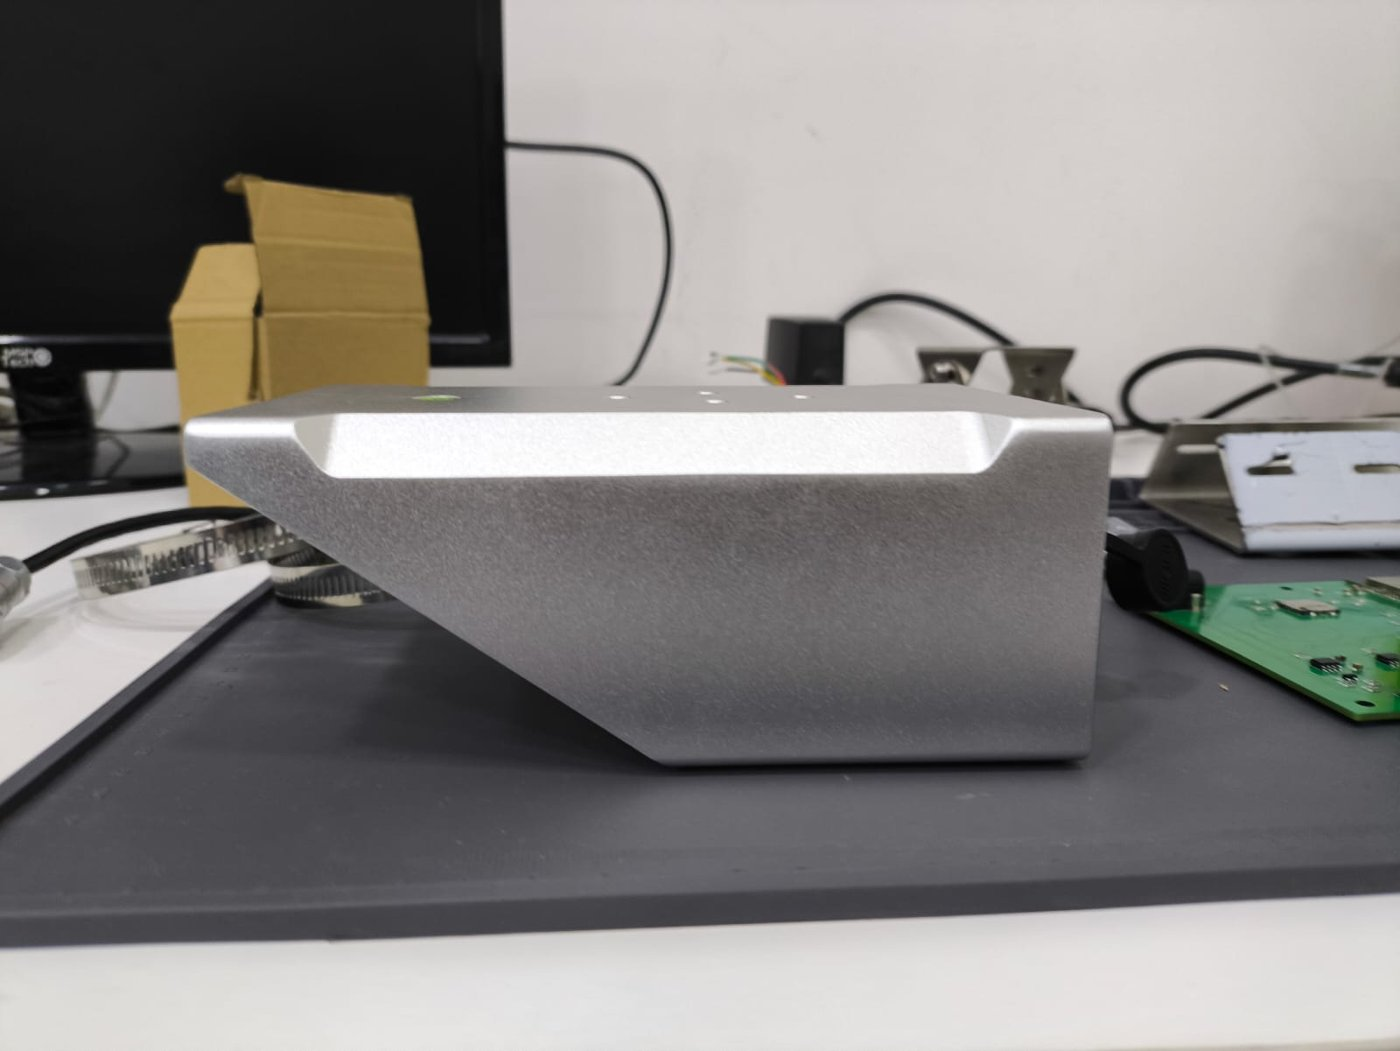
\includegraphics[height=3.8cm]{radar_sensor.jpg}
        \caption{Cuerpo del radar.}
    \end{subfigure}\hfill
    \begin{subfigure}[b]{0.2\textwidth}
        \centering
        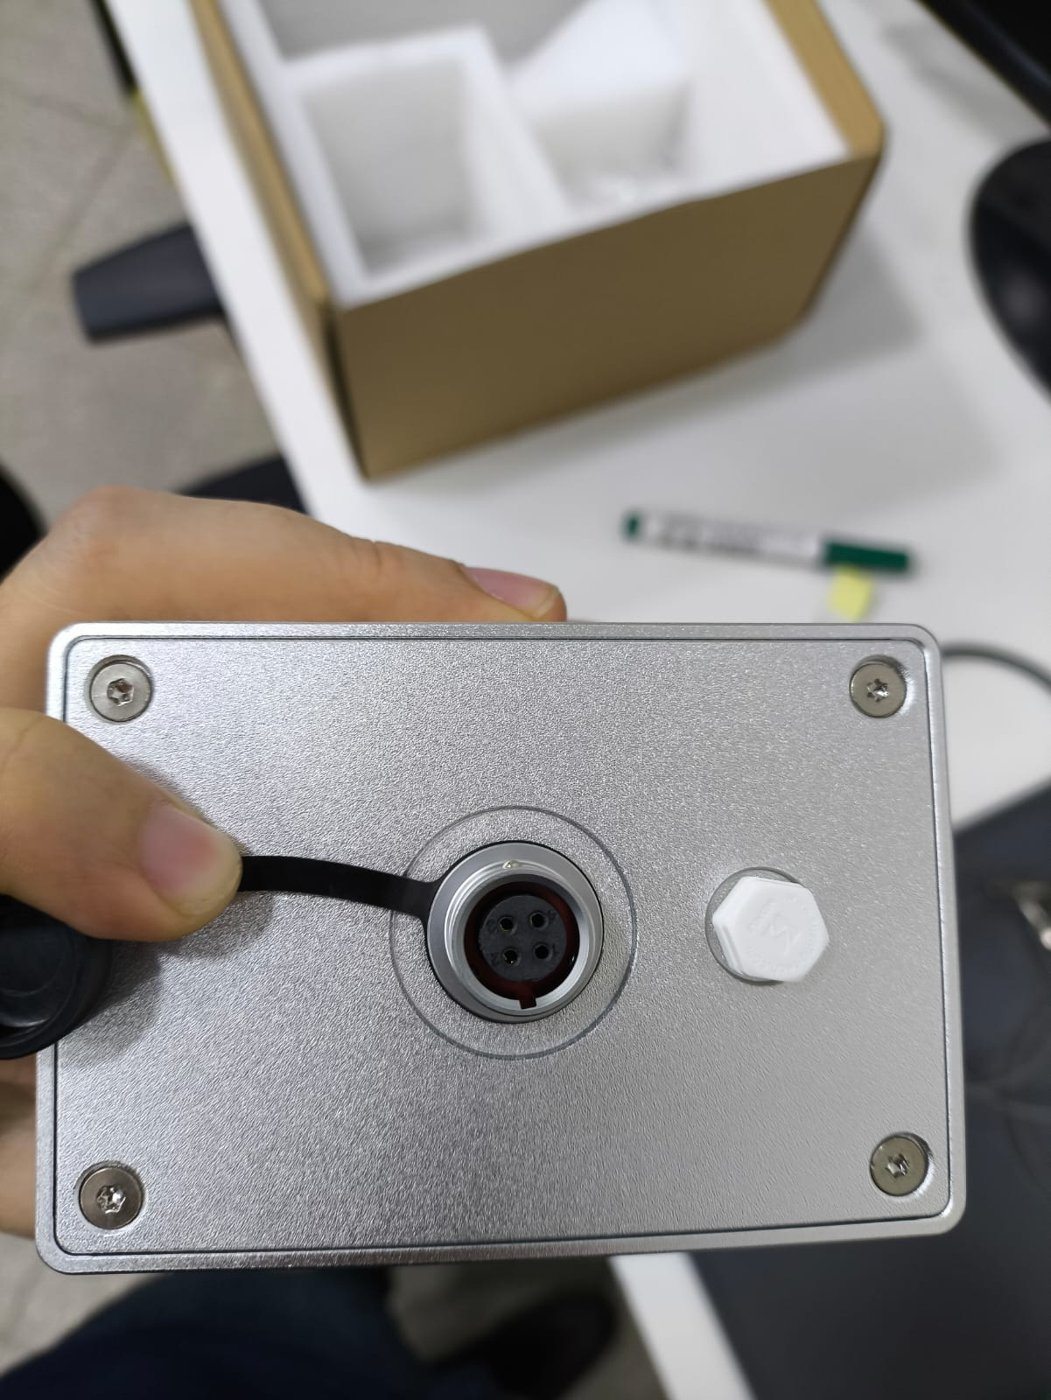
\includegraphics[height=3.8cm]{radar_conector_caja.jpg}
        \caption{Conector.}
    \end{subfigure}\hfill
    \begin{subfigure}[b]{0.2\textwidth}
        \centering
        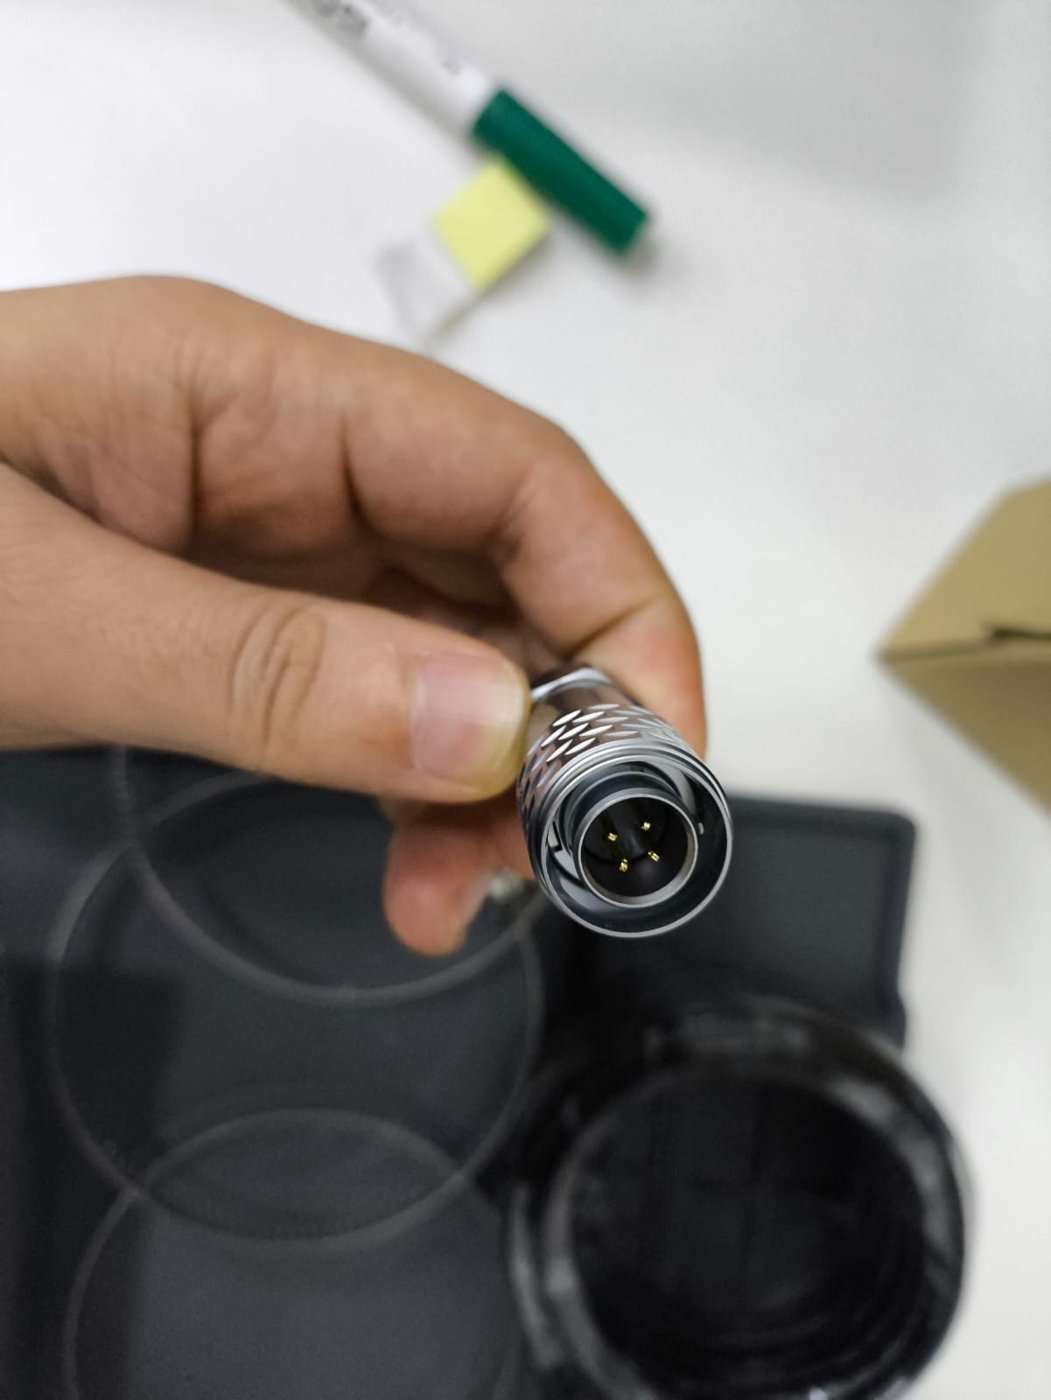
\includegraphics[height=3.8cm]{radar_ficha.jpg}
        \caption{Ficha.}
    \end{subfigure}\hfill
    \begin{subfigure}[b]{0.2\textwidth}
        \centering
        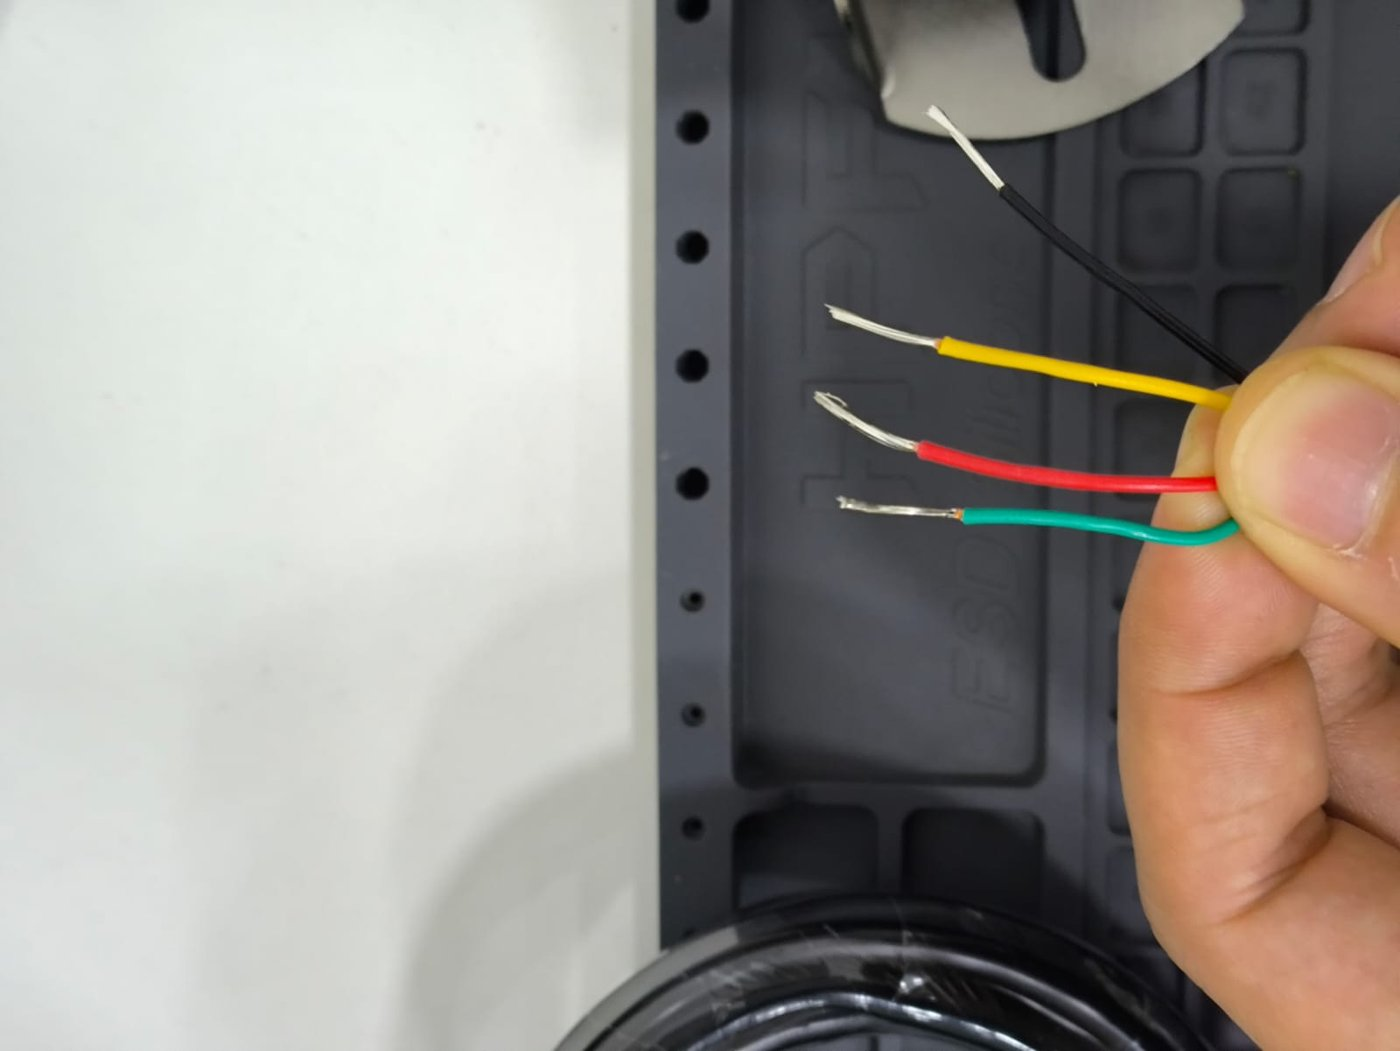
\includegraphics[height=3.8cm,trim=0 0 500 0,clip]{radar_cables.jpg}
        \caption{Hilos.}
    \end{subfigure}
    \caption{Radar FM02B: la antena de nivel mira hacia abajo y la cara
    inclinada aloja la antena de velocidad.}
\end{figure}

\textbf{Huella del haz.} Con el radar a una altura $h$ sobre el agua, el haz de
nivel ilumina una elipse de unos $0{,}25\,h \times 0{,}17\,h$ (haces de 14° y
10°)~\cite{fm02b_montaje}. Si la elipse toca una pared, la lectura es falsa.
En el banco, con un balde de 30~cm, eso limita la altura a
$h \leq 1{,}2$~m; el haz de velocidad sale a 55° de la horizontal y necesita
agua en movimiento.

\begin{figure}[!htbp]
    \centering
    \resizebox{!}{6cm}{% Haz de 14 grados del radar sobre un balde de 30 cm (escala: 1 m = 4 cm)
% Superficie del agua en y = 1.2; borde del balde en y = 1.4; medio ancho del balde 0.6
\begin{tikzpicture}[
    balde/.style={draw=gray!70!black, very thick},
    sensor/.style={fill=gray!70!black, minimum width=0.6cm, minimum height=0.35cm, inner sep=0pt},
    cota/.style={<->, >=Stealth, gray!60!black},
    rotulo/.style={font=\footnotesize, align=center}
]
    % ---------- Caso 1: sensor a 1 m del agua ----------
    \begin{scope}
        \fill[agua!25] (-0.6,0) rectangle (0.6,1.2);
        \draw[balde] (-0.6,1.4) -- (-0.6,0) -- (0.6,0) -- (0.6,1.4);
        \fill[radar!25] (0,5.2) -- (-0.49,1.2) -- (0.49,1.2) -- cycle;
        \draw[radar, thick] (-0.49,1.2) -- (0,5.2) -- (0.49,1.2);
        \node[sensor] at (0,5.38) {};
        \draw[cota] (1.0,5.2) -- node[right, rotulo] {1 m} (1.0,1.2);
        \node[rotulo, below] at (0,-0.15) {Haz de 25 cm\\\textcolor{agua!80!black}{\textbf{entra en el balde}}};
    \end{scope}

    % ---------- Caso 2: sensor a 2 m del agua ----------
    \begin{scope}[xshift=5cm]
        \fill[agua!25] (-0.6,0) rectangle (0.6,1.2);
        \draw[balde] (-0.6,1.4) -- (-0.6,0) -- (0.6,0) -- (0.6,1.4);
        \fill[radar!25] (0,9.2) -- (-0.98,1.2) -- (0.98,1.2) -- cycle;
        \draw[radar, thick] (-0.98,1.2) -- (0,9.2) -- (0.98,1.2);
        \node[sensor] at (0,9.38) {};
        \fill[red] (-0.6,1.4) circle (2.2pt) (0.6,1.4) circle (2.2pt);
        \draw[cota] (1.5,9.2) -- node[right, rotulo] {2 m} (1.5,1.2);
        \node[rotulo, below] at (0,-0.15) {Haz de 49 cm\\\textcolor{red!80!black}{\textbf{toca los bordes}}};
    \end{scope}

    % Ángulo del haz
    \node[rotulo, radar] at (5,9.95) {14°};
\end{tikzpicture}
}
    \caption{Haz de 14° sobre un balde de 30 cm, con el radar a 1 m y a 2 m.}
\end{figure}

\subsection{Conexión a la PCB}

\begin{table}[H]
    \centering
    \small
    \caption{Cableado del radar a la bornera J3.}
    \begin{tabular}{llll}
        \toprule
        \textbf{Hilo} & \textbf{Pin aviación} & \textbf{Señal} & \textbf{Borne} \\
        \midrule
        Rojo     & 1 & +12 V (9--24 V) & J3-1 \\
        Verde    & 3 & RS485 A         & J3-2 (A1) \\
        Amarillo & 4 & RS485 B         & J3-3 (B1) \\
        Negro    & 2 & GND             & J3-4 \\
        \bottomrule
    \end{tabular}
\end{table}

El canal de J3 ya tiene en la placa el transceptor SP3485 a 3,3~V,
terminación de 120~$\Omega$, polarización de 4,7~k$\Omega$ y protección TVS
SM712: no hubo que agregar nada.

\begin{figure}[!htbp]
    \centering
    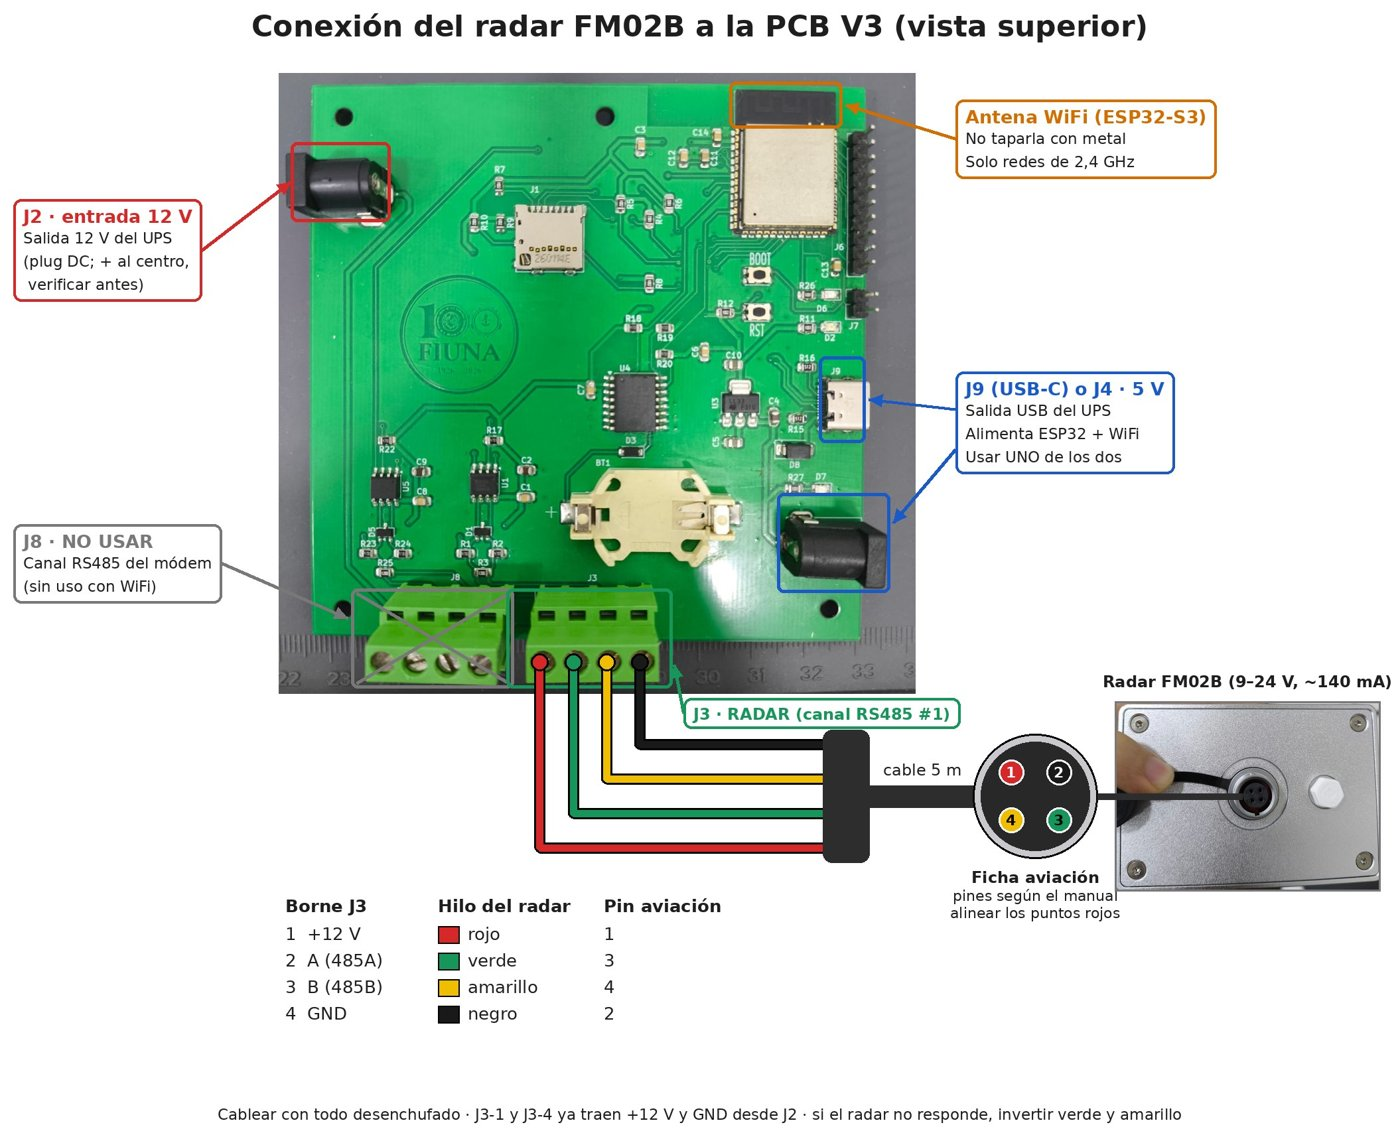
\includegraphics[width=0.95\textwidth]{diagrama_conexion_radar.jpg}
    \caption{Conexión del radar FM02B a la PCB V3 (de la guía de conexión
    elaborada por el equipo).}
\end{figure}

\subsection{Configuración leída por Bluetooth}

Antes de cablear se leyó la configuración del radar con la aplicación del
fabricante (\emph{JET Radar Debugger}). La dirección y la velocidad
coinciden con el firmware, así que no se cambió nada.

\begin{figure}[!htbp]
    \centering
    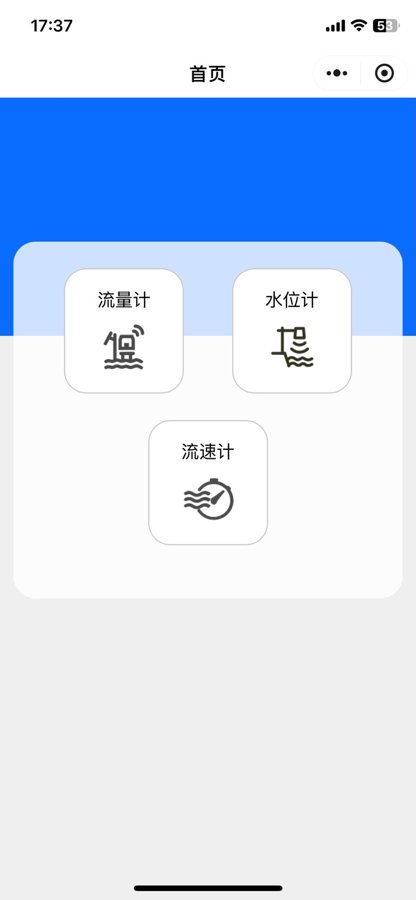
\includegraphics[width=0.19\textwidth]{app_3.jpg}\hfill
    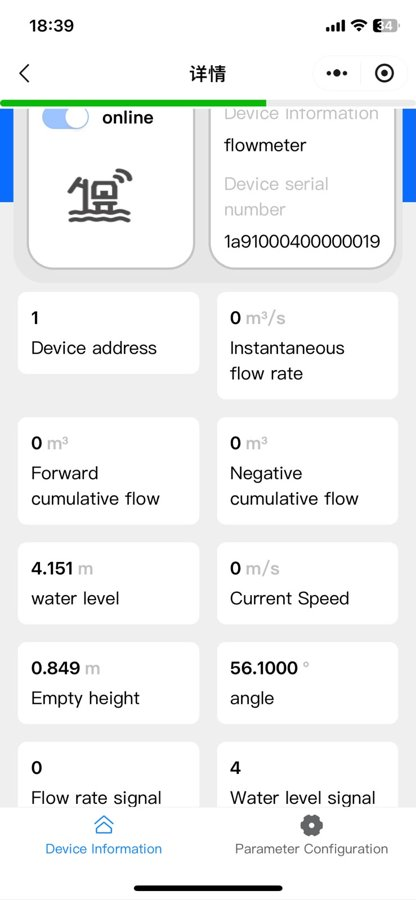
\includegraphics[width=0.19\textwidth]{app_2.jpg}\hfill
    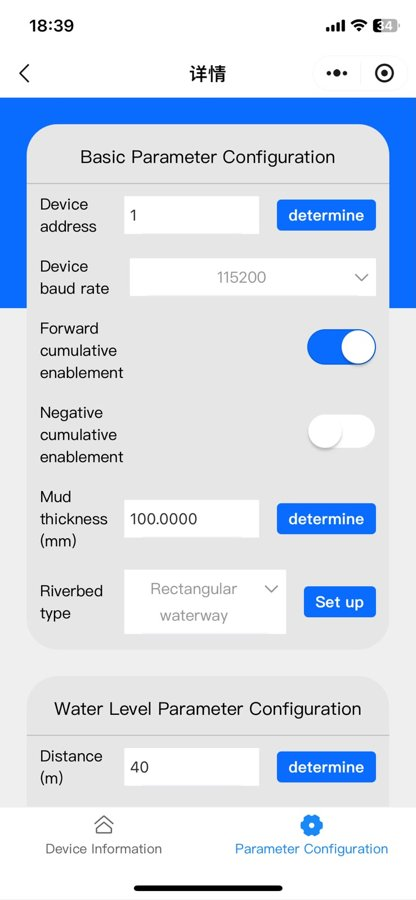
\includegraphics[width=0.19\textwidth]{app_4.jpg}\hfill
    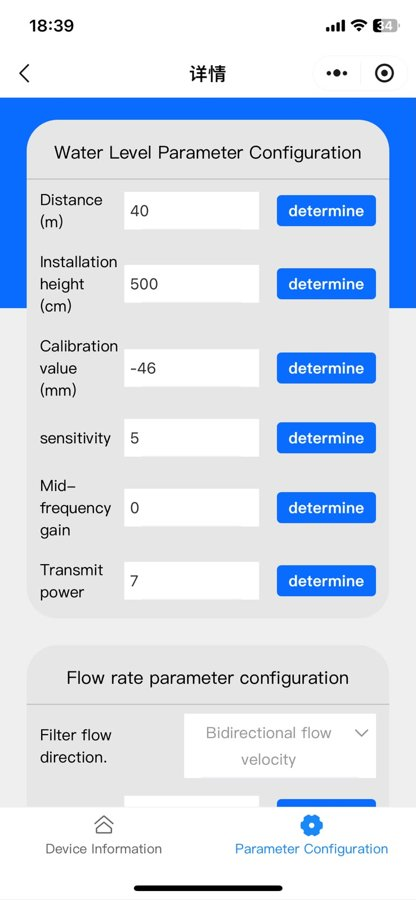
\includegraphics[width=0.19\textwidth]{app_0.jpg}\hfill
    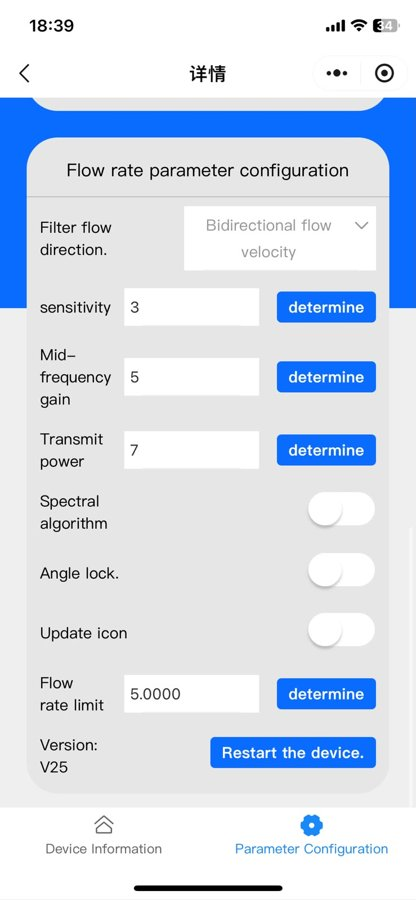
\includegraphics[width=0.19\textwidth]{app_1.jpg}
    \caption{Capturas de la aplicación: tipo de equipo, lecturas, parámetros
    básicos, de nivel y de velocidad.}
\end{figure}

\begin{table}[H]
    \centering
    \small
    \caption{Parámetros del radar leídos el 19/11/2026.}
    \begin{tabularx}{\textwidth}{>{\raggedright\arraybackslash}p{3.8cm}>{\raggedright\arraybackslash}p{2.6cm}L}
        \toprule
        \textbf{Parámetro} & \textbf{Valor} & \textbf{Comentario} \\
        \midrule
        Dirección / baudios & 1 / 115\,200 & Coinciden con el firmware. La
            tabla del manual dice 9600 de fábrica: no aplica a esta unidad. \\
        Rango de nivel & 40 m & El máximo. \\
        Calibración & $-46$ mm & Corrimiento que el radar resta a la distancia.
            Se ajusta solo si el ensayo con agua da un error constante. \\
        Potencia de emisión de nivel & 7 & La mínima (0 es la máxima). \\
        Sensibilidad de nivel & 5 & Menor valor = más sensible. \\
        Velocidad & bidireccional, límite 5 m/s & Sin cambios. \\
        \bottomrule
    \end{tabularx}
\end{table}

\subsection{Protocolo Modbus RTU}

Formato 115\,200 8N1, dirección 1, función 03 (leer registros), CRC16 Modbus
(polinomio \texttt{0xA001}). El firmware lee tres valores:

\begin{table}[H]
    \centering
    \small
    \caption{Registros del radar usados por el firmware.}
    \begin{tabular}{llll}
        \toprule
        \textbf{Registro} & \textbf{Dato} & \textbf{Trama de lectura} & \textbf{Formato} \\
        \midrule
        \texttt{0x0001} & Distancia radar--agua & \texttt{01 03 00 01 00 01 D5 CA} & uint16, mm \\
        \texttt{0x0004} & Intensidad de señal & \texttt{01 03 00 04 00 01 C5 CB} & dB ($>$ 30 buena) \\
        \texttt{0x01F4--F5} & Velocidad filtrada & \texttt{01 03 01 F4 00 02 84 05} & int32, $\times$0,001 m/s \\
        \bottomrule
    \end{tabular}
\end{table}

La respuesta a la lectura de un registro tiene 7 bytes
(\texttt{01 03 02 HH LL CRC CRC}). Otros registros útiles: \texttt{0x0009} y
\texttt{0x000A} (inclinación en 0,1°, para comprobar que el radar no se movió),
\texttt{0x07D8} (calibración), \texttt{0x07D7} (potencia) y \texttt{0x07D9}
(sensibilidad).

% ======================================================
% 7. FIRMWARE
% ======================================================
\seccion{Firmware}

El firmware se escribió en C con ESP-IDF~5.5 sobre PlatformIO y está
organizado en componentes. Se conserva el esquema de Proyecto~3: un ciclo
principal que mide en turnos fijos y una tarea en segundo plano que reenvía
los pendientes. Lo nuevo se resume en la tabla.

\begin{table}[H]
    \centering
    \small
    \caption{Cambios del firmware para el segundo parcial.}
    \begin{tabularx}{\textwidth}{>{\raggedright\arraybackslash}p{3.2cm}LL}
        \toprule
        \textbf{Tema} & \textbf{Antes (ultrasónico, P3)} & \textbf{Ahora (radar)} \\
        \midrule
        Sensor & 9600 baudios, registro \texttt{0x0000}, sin verificar el CRC. &
            115\,200, registros \texttt{0x0001}, \texttt{0x0004} y
            \texttt{0x01F4}; verifica CRC, dirección, función y largo. \\
        Control DE/RE & Por software, con retardos. & Por hardware (UART en
            modo RS485 \emph{half-duplex}). \\
        Falla del sensor & Se enviaba $-1$ sin más datos. & Además, un
            \textbf{estado}: sin respuesta, respuesta inválida o fuera de
            rango ($<$ 0,1 m). \\
        Identificación & El id lo ponía el servidor. & \textbf{id
            correlativo} guardado en la memoria NVS: sobrevive a reinicios. \\
        microSD & Dos tareas escribían sin protección. & \emph{Mutex},
            \texttt{fflush} + \texttt{fsync} y recuperación de la cola tras un
            corte. \\
        Envío & Módem GPRS. & WiFi o módem GPRS. \\
        Hora & Solo el RTC. & NTP al arrancar; sin hora válida no se mide. \\
        Pruebas & -- & \textbf{Modo banco}: lee el radar cada 2 s y lo
            muestra, sin guardar ni enviar. \\
        \bottomrule
    \end{tabularx}
\end{table}

\subsection{Flujo del programa}

\begin{figure}[!htbp]
    \centering
    \resizebox{0.98\textwidth}{!}{% Arranque y ciclo principal del firmware (2.o parcial)
\begin{tikzpicture}[
    node distance=0.42cm,
    paso/.style={draw=gray!60!black, fill=white, rounded corners=2pt, align=center,
        font=\footnotesize, text width=4.8cm, minimum height=0.7cm, inner sep=3pt},
    nuevo/.style={paso, draw=radar!80!black, fill=radar!8},
    dec/.style={diamond, aspect=2.4, draw=gray!60!black, fill=gray!8, align=center,
        font=\footnotesize, inner sep=0.5pt},
    ini/.style={paso, rounded corners=8pt, fill=agua!15, draw=agua!70!black, font=\footnotesize\bfseries},
    lado/.style={paso, text width=3.0cm},
    flecha/.style={-{Stealth}, thick, gray!60!black},
    si/.style={font=\scriptsize\bfseries, text=agua!60!black},
    no/.style={font=\scriptsize\bfseries, text=red!70!black}
]
    % ---------- Arranque ----------
    \node[ini] (a0) {INICIO};
    \node[paso, below=of a0] (a1) {Inicializar RTC, microSD,\\radar (UART1 115200), módem (UART2), WiFi y LED};
    \node[paso, below=of a1] (a2) {Crear mutex de envío};
    \node[nuevo, below=of a2] (a3) {Sincronizar RTC por NTP\\(si hay WiFi)};
    \node[paso, below=of a3] (a4) {Crear tarea de pendientes\\en segundo plano};
    \foreach \i/\j in {a0/a1,a1/a2,a2/a3,a3/a4} \draw[flecha] (\i) -- (\j);
    \node[font=\small\bfseries, above=0.15cm of a0] {Arranque};

    % ---------- Ciclo ----------
    \begin{scope}[xshift=12cm]
    \node[ini] (b0) {CICLO PRINCIPAL};
    \node[paso, below=of b0] (b1) {Leer hora del RTC};
    \node[dec, below=of b1] (b2) {¿Hora válida?\\(año $\geq$ 2025)};
    \node[dec, below=of b2] (b3) {¿Llegó el\\turno de 5 min?};
    \node[nuevo, below=of b3] (b4) {id = id + 1 (memoria NVS)};
    \node[paso, below=of b4] (b5) {Leer radar: distancia, señal\\y velocidad (hasta 3 intentos)};
    \node[dec, below=of b5] (b6) {¿Lectura OK?};
    \node[nuevo, below=of b6] (b7) {Guardar en \texttt{datos.csv}:\\epoch, id, d, v, señal, estado};
    \node[nuevo, below=of b7] (b8) {Enviar \texttt{d=epoch,valor} por módem GPRS; si no hay OK, por WiFi (con mutex)};
    \node[dec, below=of b8] (b9) {¿OK por algún\\medio?};
    \node[nuevo, below=of b9] (b10) {Línea completa a la PC (UDP) y a la página (HTTPS)};

    \node[lado, nuevo, left=0.9cm of b2] (n2) {No medir: reintentar NTP cada 60 s};
    \node[lado, left=0.9cm of b3] (n3) {Esperar los segundos que faltan};
    \node[lado, left=0.9cm of b6] (n6) {valor = $-1$, estado $\neq$ 0\\(LED apagado)};
    \node[lado, right=0.9cm of b6] (s6) {Parpadeo del LED};
    \node[lado, left=0.9cm of b9] (n9) {Guardar en \texttt{temp.csv}\\(pendiente)};

    \foreach \i/\j in {b0/b1,b1/b2,b4/b5,b5/b6,b7/b8,b8/b9} \draw[flecha] (\i) -- (\j);
    \draw[flecha] (b2) -- node[si, right] {sí} (b3);
    \draw[flecha] (b3) -- node[si, right] {sí} (b4);
    \draw[flecha] (b6) -- node[si, right, pos=0.4] {} (b7);
    \draw[flecha] (b9) -- node[si, right] {sí} (b10);
    \draw[flecha] (b2) -- node[no, above] {no} (n2);
    \draw[flecha] (b3) -- node[no, above] {no} (n3);
    \draw[flecha] (b6) -- node[no, above] {no} (n6);
    \draw[flecha] (b6) -- node[si, above] {sí} (s6);
    \draw[flecha] (b9) -- node[no, above] {no} (n9);
    \draw[flecha] (n6) |- (b7.west);
    \draw[flecha] (s6) |- (b7.east);
    \draw[flecha] (n9) |- (b10.west);
    \draw[flecha] (n2.north) |- ([yshift=-0.15cm]b1.west);
    % rodea por fuera el cuadro "No medir" (n2), que está más a la izquierda
    \draw[flecha] (n3.west) -- ($(n2.west |- n3.west)+(-0.35,0)$) |- ([yshift=0.15cm]b1.west);
    \draw[flecha] (b10.east) -- ++(4.3,0) |- (b1.east);
    \end{scope}

    % conexión arranque -> ciclo
    \draw[flecha] (a4.east) -- ++(0.5,0) |- (b0.west);

    % Leyenda
    \node[nuevo, text width=2.4cm, below=1.2cm of a4] (ley) {nuevo en el\\2.\textsuperscript{o} parcial};
\end{tikzpicture}
}
    \caption{Arranque y ciclo principal. En azul, lo nuevo de este parcial.}
\end{figure}

Cuando el envío falla, el dato queda en \texttt{temp.csv}. La tarea de
pendientes lo reenvía en orden (FIFO) y lo borra recién cuando el servidor
confirma con \texttt{OK}. Para no chocar con el ciclo principal, solo trabaja
si faltan más de 35~s para el próximo turno, y ya no intenta enviar si no hay
conexión.

\begin{figure}[!htbp]
    \centering
    \resizebox{0.78\textwidth}{!}{% Tarea de pendientes (Store and Forward) en segundo plano
\begin{tikzpicture}[
    node distance=0.42cm,
    paso/.style={draw=gray!60!black, fill=white, rounded corners=2pt, align=center,
        font=\footnotesize, text width=4.3cm, minimum height=0.7cm, inner sep=3pt},
    nuevo/.style={paso, draw=radar!80!black, fill=radar!8},
    dec/.style={diamond, aspect=2.6, draw=gray!60!black, fill=gray!8, align=center,
        font=\footnotesize, inner sep=0.5pt},
    ini/.style={paso, rounded corners=8pt, fill=agua!15, draw=agua!70!black, font=\footnotesize\bfseries},
    lado/.style={paso, text width=3.1cm},
    flecha/.style={-{Stealth}, thick, gray!60!black},
    si/.style={font=\scriptsize\bfseries, text=agua!60!black},
    no/.style={font=\scriptsize\bfseries, text=red!70!black}
]
    \node[ini, text width=5.6cm] (c0) {TAREA DE PENDIENTES (cada 5 s)};
    \node[dec, below=of c0] (c1) {¿Faltan $>$ 35 s\\para el próximo turno?};
    \node[dec, below=of c1, fill=radar!8, draw=radar!80!black] (c2) {¿Hay conexión?};
    \node[dec, below=of c2] (c3) {¿Hay datos en\\\texttt{temp.csv}?};
    \node[dec, below=of c3, fill=radar!8, draw=radar!80!black] (c4) {¿Fecha válida?};
    \node[paso, below=of c4] (c5) {Reenviar el primero (FIFO)\\\texttt{d=epoch,valor}, con mutex};
    \node[dec, below=of c5] (c6) {¿Respuesta OK?};
    \node[nuevo, below=of c6] (c7) {Quitarlo de la cola\\(copia \texttt{temp\_aux.csv} + \texttt{fsync})};

    \node[lado, right=1.0cm of c2] (esp) {Esperar 5 s y volver};
    \node[lado, nuevo, left=1.0cm of c4] (desc) {Descartar\\(dato con fecha del año 2000)};
    \node[lado, right=1.0cm of c6] (cons) {Conservar en la cola};

    \foreach \i/\j in {c0/c1,c5/c6} \draw[flecha] (\i) -- (\j);
    \draw[flecha] (c1) -- node[si, right] {sí} (c2);
    \draw[flecha] (c2) -- node[si, right] {sí} (c3);
    \draw[flecha] (c3) -- node[si, right] {sí} (c4);
    \draw[flecha] (c4) -- node[si, right] {sí} (c5);
    \draw[flecha] (c6) -- node[si, right] {sí} (c7);
    \draw[flecha] (c1.east) -| node[no, above, pos=0.2] {no} (esp.north);
    \draw[flecha] (c2) -- node[no, above] {no} (esp);
    \draw[flecha] (c3.east) -| node[no, below, pos=0.2] {no} (esp.south);
    \draw[flecha] (c4) -- node[no, above] {no} (desc);
    \draw[flecha] (c6) -- node[no, above] {no} (cons);
    \draw[flecha] (cons.east) -| ([xshift=1.0cm]esp.east);
    \draw[flecha] (c7.east) -| ([xshift=1.0cm]esp.east) |- (esp.east);
    \draw[flecha] (desc.south) |- (c7.west);
\end{tikzpicture}
}
    \caption{Tarea de pendientes (\emph{Store and Forward}).}
\end{figure}

\subsection{Trama y registro en la microSD}
\label{sec:trama}

En el primer parcial se propuso enviar al servidor la trama
\begin{center}\texttt{d=<epoch>,<id>,<distancia>,<velocidad>,<estado>}\end{center}
Como el script del
servidor no se puede modificar y acepta solo dos campos, \textbf{al servidor
sigue yendo la trama de siempre} y el registro completo se guarda en la
microSD. Así, los perdidos y duplicados se verifican cruzando el id de la
microSD con la base de datos; como los turnos son fijos, también se detectan
por la hora. La trama nueva queda lista para cuando el administrador habilite
un script nuevo.

\begin{figure}[!htbp]
    \centering
    % Trama al servidor y registro completo en la microSD
\begin{tikzpicture}[
    campo/.style={draw=gray!70, fill=white, minimum height=0.65cm, inner sep=3pt, font=\footnotesize\ttfamily},
    nuevo/.style={campo, draw=radar, fill=radar!10},
    nota/.style={font=\scriptsize, text=gray!60!black, align=center}
]
    \node[anchor=west, font=\small\bfseries] at (0,0.9) {Al servidor (sin cambios; módem GPRS o WiFi)};
    \node[campo, anchor=west] (a1) at (0,0) {d=};
    \node[campo, right=0pt of a1] (a2) {epoch UTC};
    \node[campo, right=0pt of a2] (a3) {distancia (m)};
    \node[nota, right=8pt of a3] {ej.: \texttt{d=1795144800,0.864}\\$-1$ si el radar falla};

    \node[anchor=west, font=\small\bfseries] at (0,-1.6) {En la microSD, a la PC y a la página: línea de \texttt{datos.csv} (nuevo)};
    \node[campo, anchor=west] (b1) at (0,-2.5) {epoch};
    \node[nuevo, right=0pt of b1] (b2) {id};
    \node[campo, right=0pt of b2] (b3) {distancia\_m};
    \node[nuevo, right=0pt of b3] (b4) {velocidad\_ms};
    \node[nuevo, right=0pt of b4] (b5) {senal\_db};
    \node[nuevo, right=0pt of b5] (b6) {estado};
    \node[nota, below=3pt of b2] {correlativo\\(NVS)};
    \node[nota, below=3pt of b4] {reg.\\\texttt{0x01F4}};
    \node[nota, below=3pt of b5] {reg.\\\texttt{0x0004}};
    \node[nota, right=6pt of b6] {0 OK, 1 sin respuesta,\\2 inválida, 3 fuera de rango};
    \node[nota, anchor=west, font=\footnotesize] at (0,-4.15) {ej.: \texttt{1795144800,2,0.864,0.000,18,0}};
\end{tikzpicture}

    \caption{Trama enviada al servidor y registro completo en la microSD.}
\end{figure}

Cada línea de \texttt{datos.csv} pesa unos 32 bytes. A 288 lecturas por día son
unos 9~kB diarios y 3,4~MB por año: la capacidad de la tarjeta de 32~GB no es
un límite.

\subsection{Protecciones agregadas}

\begin{itemize}
    \item \textbf{Hora inválida.} En la primera prueba el RTC estaba en el año
        2000 y llegaron al servidor datos con esa fecha. Ahora el RTC se
        sincroniza por NTP al arrancar, no se mide si el año es anterior a
        2025, y los pendientes con fecha inválida se descartan.
    \item \textbf{Cortes de energía.} Cada escritura termina con
        \texttt{fsync}. Para quitar un pendiente se reescribe la cola en un
        archivo auxiliar y se reemplaza; si la energía se corta a mitad de
        camino, al arrancar se recupera la cola completa.
    \item \textbf{Acceso concurrente.} Un mutex protege la microSD y otro el
        envío, porque el ciclo principal y la tarea de pendientes los usan a
        la vez.
\end{itemize}

\subsection{Modo banco}

Para los ensayos de exactitud el firmware se compila con la opción
\texttt{-DMODO\_BANCO}: lee el radar cada 2~s y muestra distancia, señal y
velocidad en el monitor serie, sin guardar ni enviar. El intervalo de
producción (5~min) también se puede cambiar al compilar, lo que permitió hacer
el ensayo de corte de red con turnos de 1~min.

\begin{verbatim}
PLATFORMIO_BUILD_FLAGS=-DMODO_BANCO pio run -t upload
SENSOR_RS485: Distancia: 0.864 m | senal: 18 dB | velocidad: 0.000 m/s
\end{verbatim}

% ======================================================
% 8. DISENO ELECTRONICO
% ======================================================
\seccion{Diseño electrónico}

El diseño electrónico es el del primer parcial: una PCB propia de dos capas,
dividida en subsistemas. Para el radar no hizo falta modificarla.

\begin{table}[H]
    \centering
    \small
    \caption{Subsistemas de la PCB.}
    \begin{tabularx}{\textwidth}{>{\raggedright\arraybackslash}p{3.2cm}L}
        \toprule
        \textbf{Subsistema} & \textbf{Función} \\
        \midrule
        Alimentación & Regulador AMS1117 de 5 V a 3,3 V; 12 V directo a las
            borneras RS485. \\
        ESP32-S3 & Ejecuta el firmware, coordina los periféricos y el WiFi. \\
        RTC DS3231M & Fecha y hora de cada medición (I2C), con pila CR2032. \\
        microSD & Historial y cola de pendientes (SPI). \\
        USB-C & Alimentación, programación y monitor serie. \\
        TTL-RS485 & Dos SP3485: radar (J3) y módem (J8). \\
        \bottomrule
    \end{tabularx}
\end{table}

\begin{figure}[!htbp]
    \centering
    \begin{subfigure}[b]{0.48\textwidth}
        \centering
        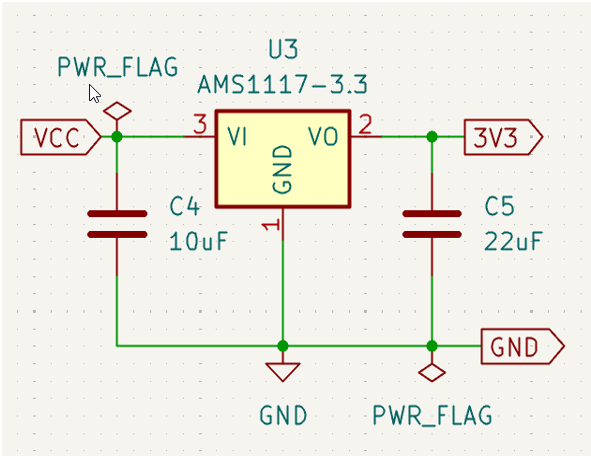
\includegraphics[width=\textwidth]{esq_alimentacion.png}
        \caption{Alimentación.}
    \end{subfigure}\hfill
    \begin{subfigure}[b]{0.48\textwidth}
        \centering
        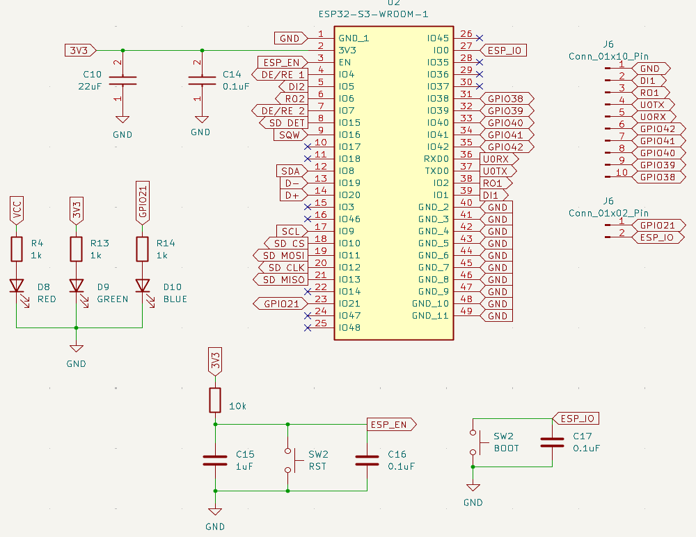
\includegraphics[width=\textwidth]{esq_esp32.png}
        \caption{ESP32-S3.}
    \end{subfigure}\\[6pt]
    \begin{subfigure}[b]{0.48\textwidth}
        \centering
        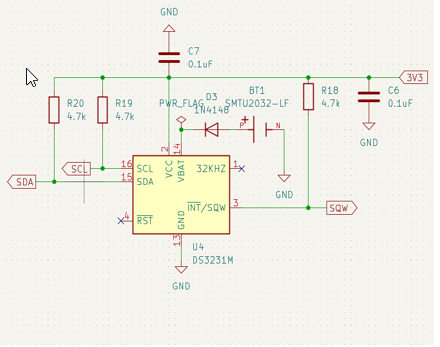
\includegraphics[width=\textwidth]{esq_rtc.png}
        \caption{RTC DS3231M.}
    \end{subfigure}\hfill
    \begin{subfigure}[b]{0.48\textwidth}
        \centering
        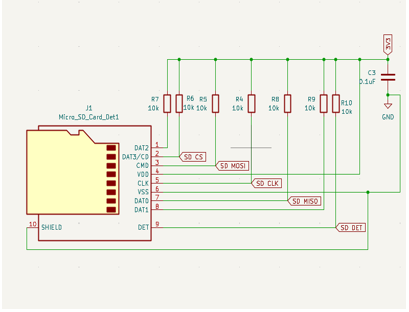
\includegraphics[width=\textwidth]{esq_sd.png}
        \caption{microSD.}
    \end{subfigure}\\[6pt]
    \begin{subfigure}[b]{0.42\textwidth}
        \centering
        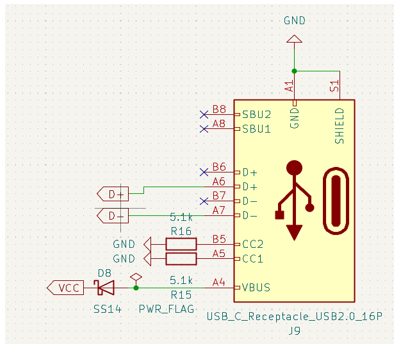
\includegraphics[width=\textwidth]{esq_usbc.png}
        \caption{USB-C.}
    \end{subfigure}\hfill
    \begin{subfigure}[b]{0.52\textwidth}
        \centering
        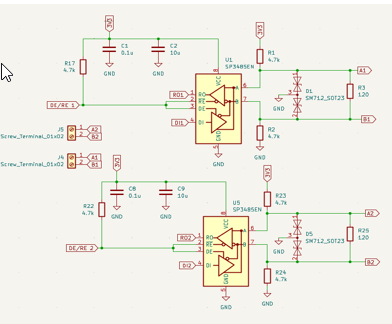
\includegraphics[width=\textwidth]{esq_rs485.png}
        \caption{Transceptores TTL-RS485.}
    \end{subfigure}
    \caption{Esquemas de los subsistemas.}
\end{figure}

\subsection{Placa}

La placa se planteó primero en cuatro capas y se rediseñó en dos para
simplificar la fabricación, reducir el costo y facilitar la inspección. El
montaje se hizo con pasta de soldar y horno de reflujo~\cite{horno}.

\begin{figure}[!htbp]
    \centering
    \begin{subfigure}[b]{0.32\textwidth}
        \centering
        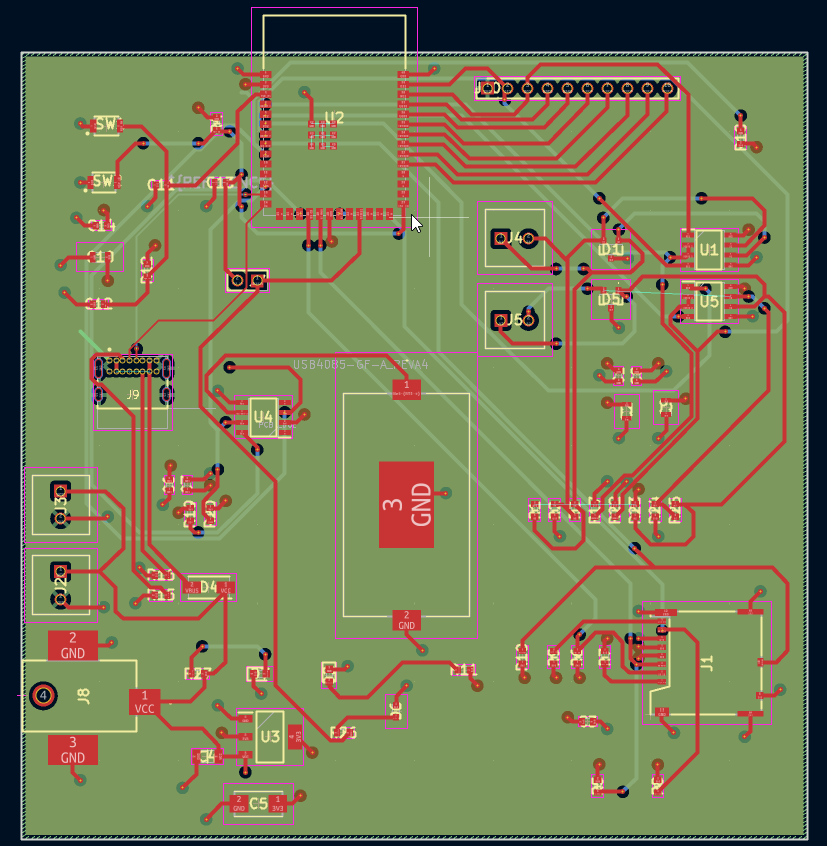
\includegraphics[width=\textwidth]{pcb_4capas.png}
        \caption{Diseño inicial, 4 capas.}
    \end{subfigure}\hfill
    \begin{subfigure}[b]{0.32\textwidth}
        \centering
        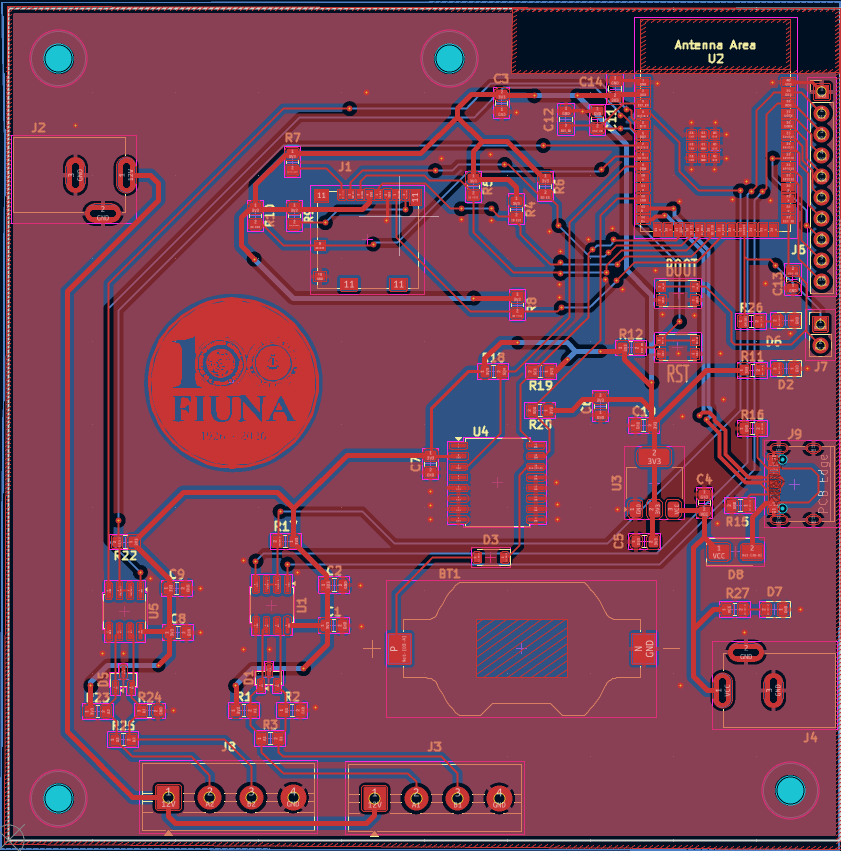
\includegraphics[width=\textwidth]{pcb_2capas.png}
        \caption{Diseño final, 2 capas.}
    \end{subfigure}\hfill
    \begin{subfigure}[b]{0.32\textwidth}
        \centering
        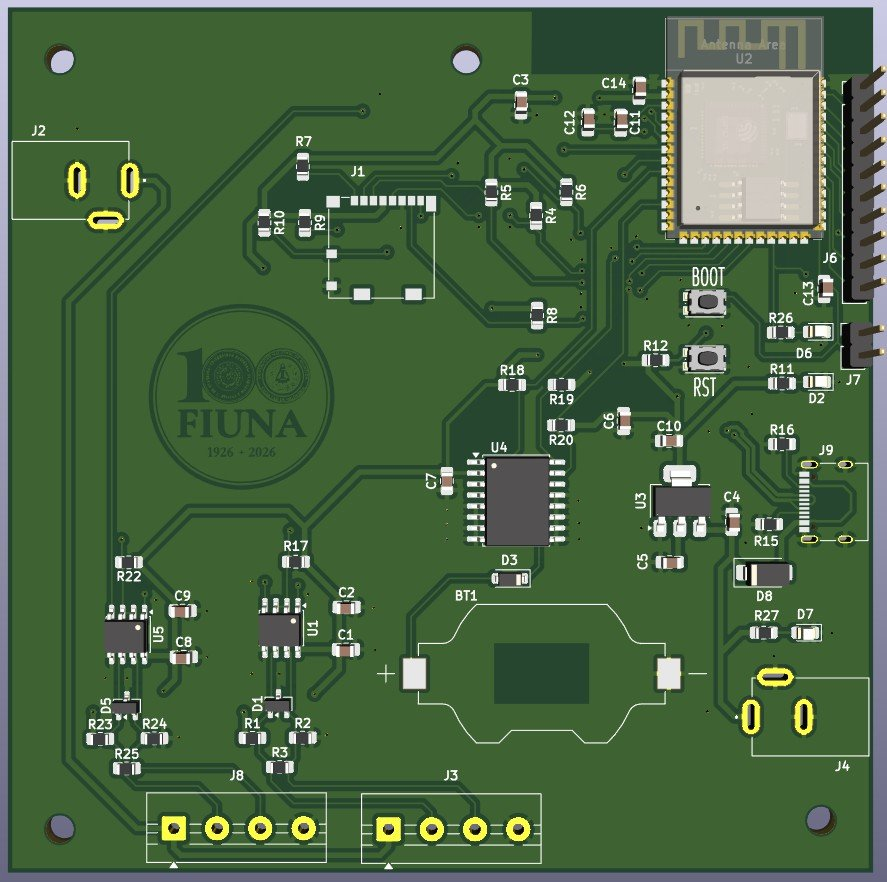
\includegraphics[width=\textwidth]{pcb3d_front_fin.jpg}
        \caption{Vista 3D del diseño final.}
    \end{subfigure}
    \caption{Evolución del diseño de la PCB.}
\end{figure}

\begin{figure}[!htbp]
    \centering
    \begin{subfigure}[b]{0.48\textwidth}
        \centering
        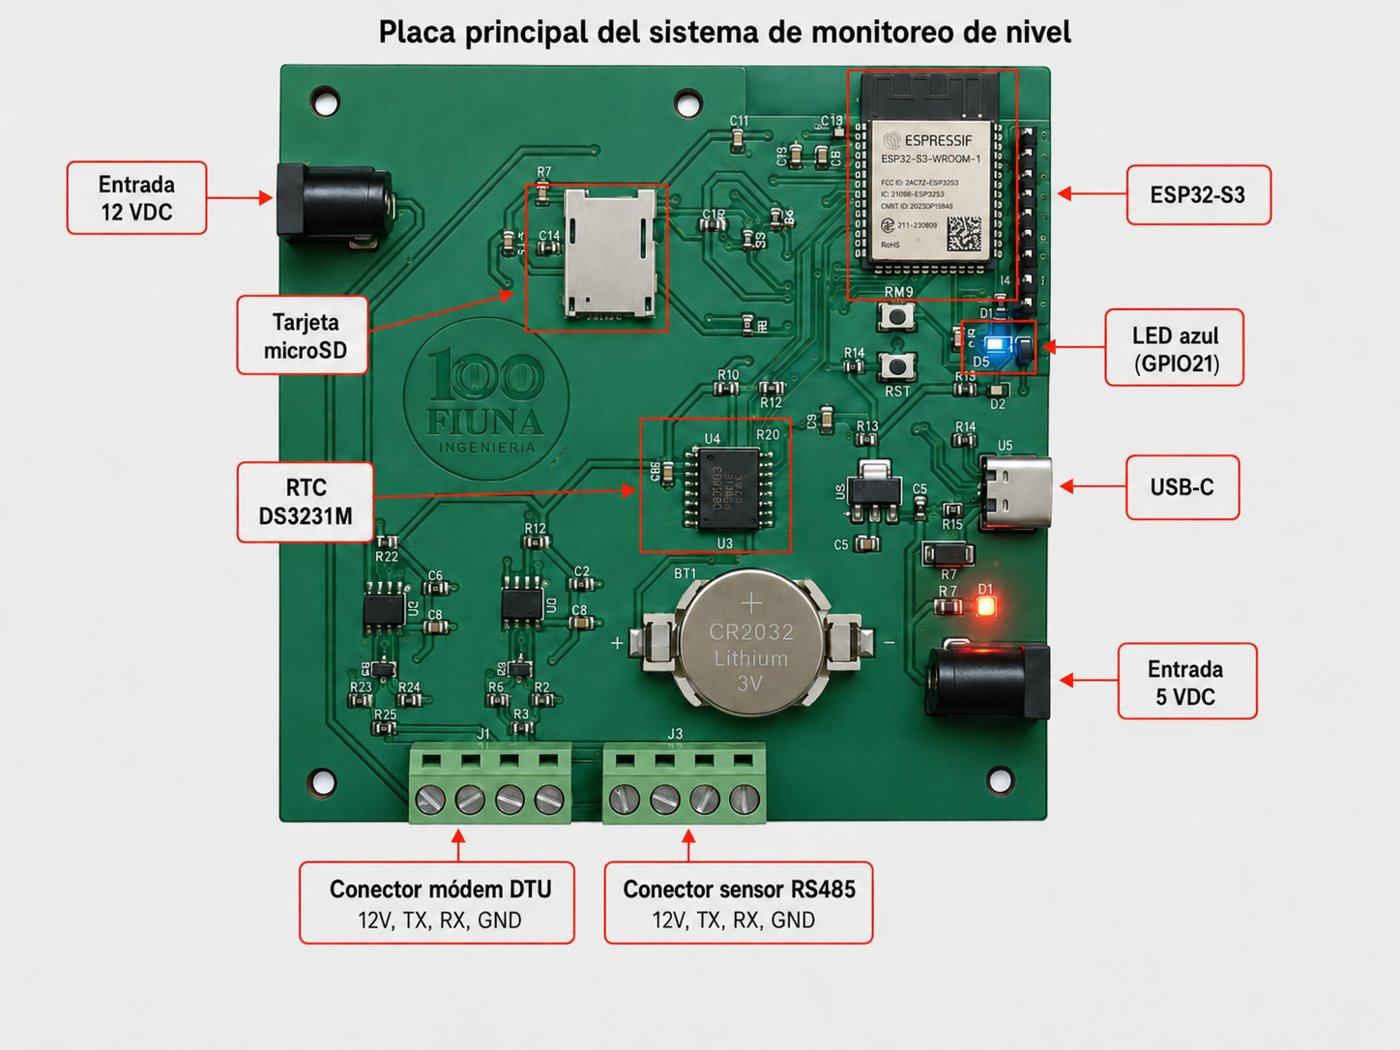
\includegraphics[width=\textwidth]{pcb_partes.jpg}
        \caption{Partes principales.}
    \end{subfigure}\hfill
    \begin{subfigure}[b]{0.42\textwidth}
        \centering
        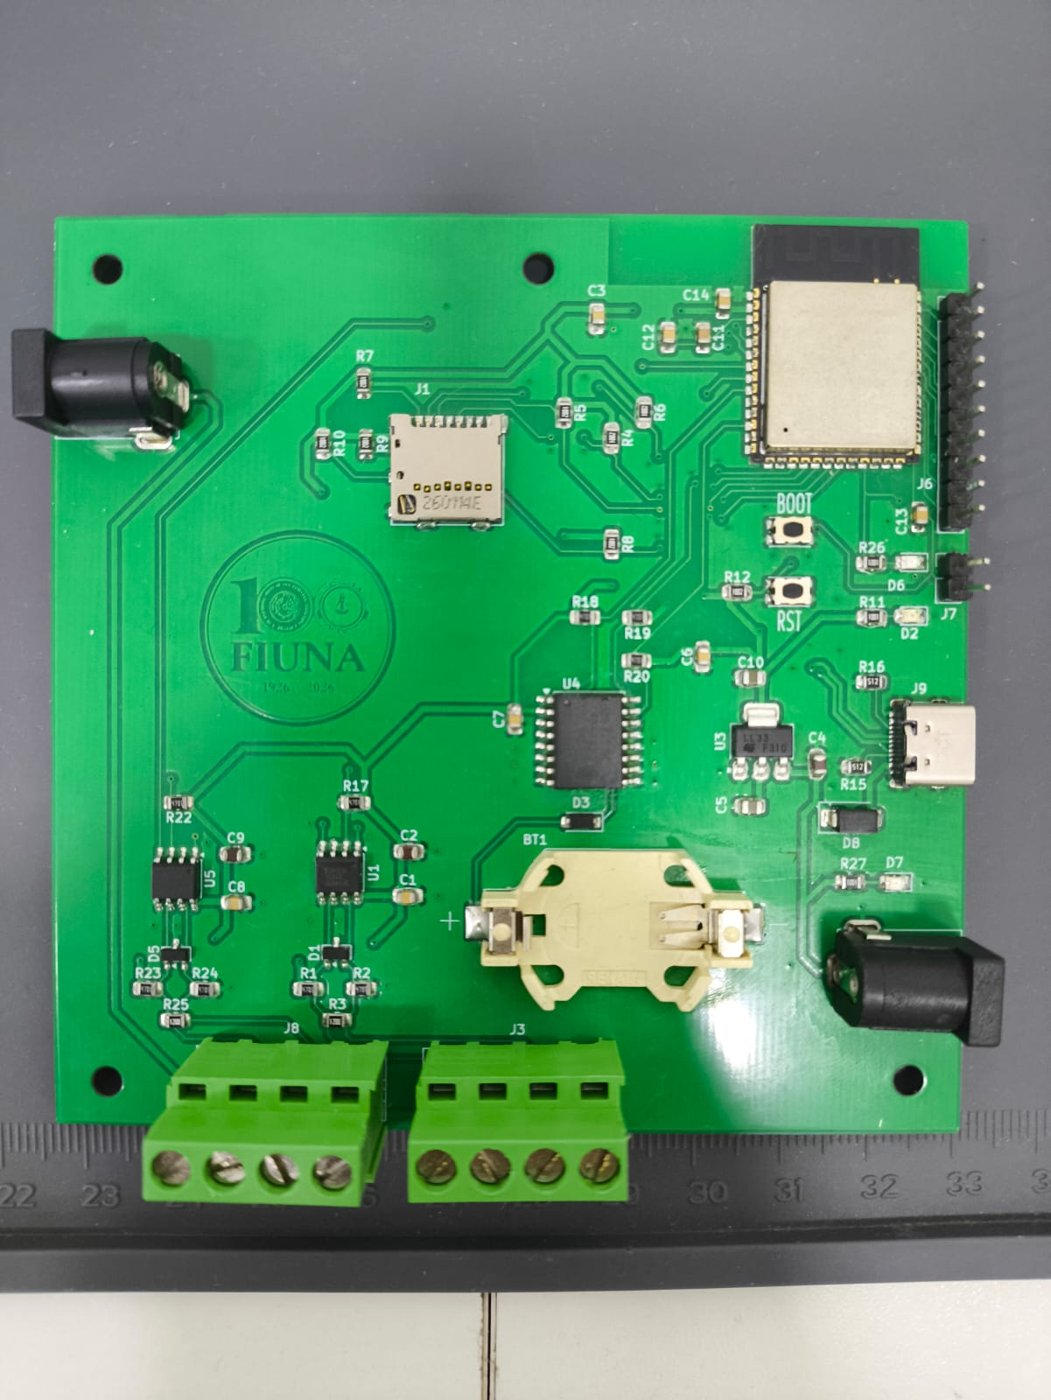
\includegraphics[width=\textwidth]{placa_v3.jpg}
        \caption{Placa usada con el radar.}
    \end{subfigure}
    \caption{PCB montada.}
\end{figure}

\begin{table}[H]
    \centering
    \small
    \caption{Conectores de la placa.}
    \begin{tabular}{lll}
        \toprule
        \textbf{Conector} & \textbf{Qué es} & \textbf{Uso actual} \\
        \midrule
        J2 & Jack DC, entrada 12 V & Salida 12 V de la UPS (solo alimenta las borneras) \\
        J9 & USB-C, 5 V (con diodo) & Salida USB de la UPS; programación \\
        J4 & Jack DC, 5 V & Alternativa a J9 (usar uno solo) \\
        J3 & Bornera 4 polos, RS485 \#1 & Radar FM02B \\
        J8 & Bornera 4 polos, RS485 \#2 & Módem DTU (modo módem) \\
        \bottomrule
    \end{tabular}
\end{table}

\subsection{Sistema de control}
La estación no controla una variable física: es un sistema de adquisición,
almacenamiento y transmisión. Lo que sí implementa es la lógica de flujo del
programa: temporización por turnos, validación de cada lectura, reintentos,
manejo de fallas de comunicación y exclusión mutua entre tareas.

% ======================================================
% 9. DISENO MECANICO
% ======================================================
\seccion{Diseño mecánico}

\subsection{Diseño del primer parcial}

En el primer parcial se diseñaron en SolidWorks el gabinete de la electrónica
(PCB, UPS y módem, con el cableado por el perímetro y tapa desmontable) y un
soporte de acero para el sensor ultrasónico. Con el cambio al radar, el soporte
propio se reemplaza por el kit del fabricante; el gabinete sigue siendo válido
para alojar la electrónica.

\begin{figure}[!htbp]
    \centering
    \begin{subfigure}[b]{0.32\textwidth}
        \centering
        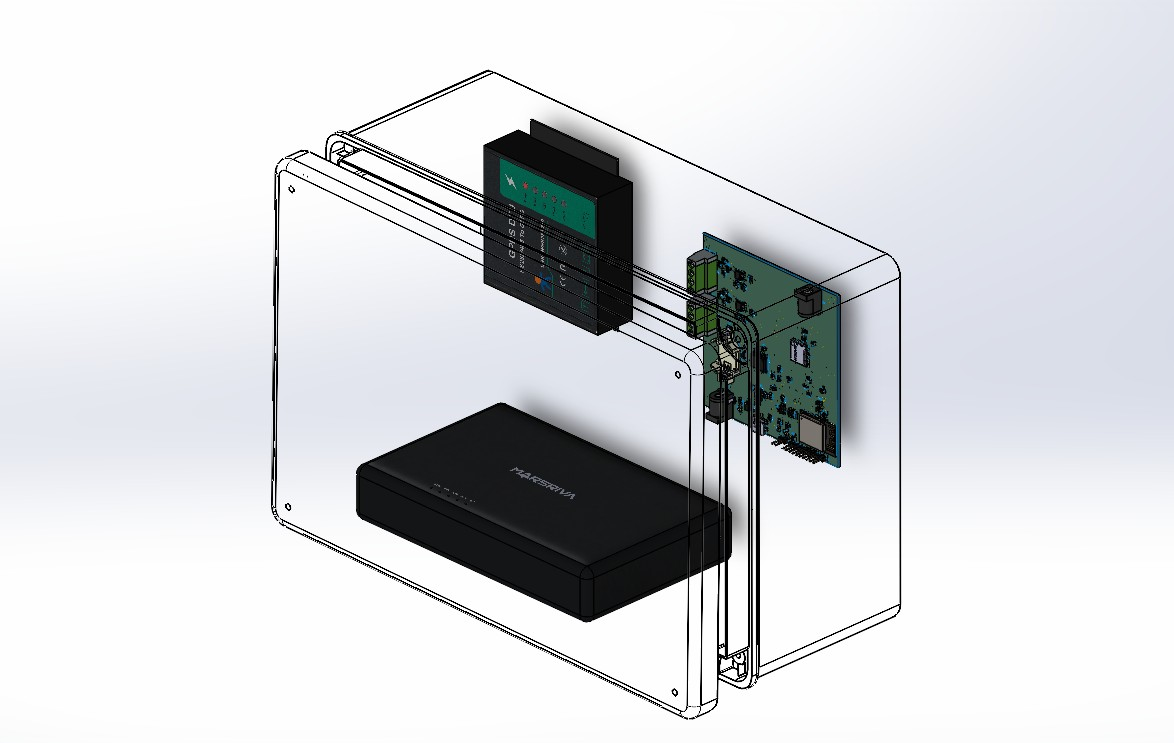
\includegraphics[width=\textwidth]{cad_caja_dist.png}
        \caption{Distribución interna.}
    \end{subfigure}\hfill
    \begin{subfigure}[b]{0.32\textwidth}
        \centering
        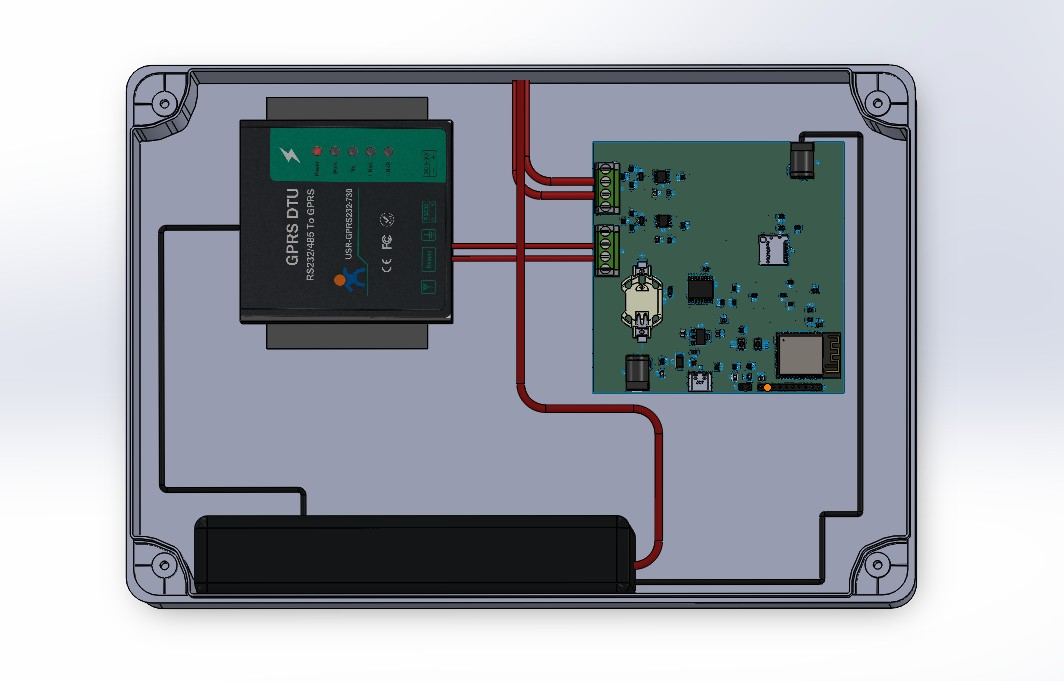
\includegraphics[width=\textwidth]{cad_caja_cableado.png}
        \caption{Recorrido del cableado.}
    \end{subfigure}\hfill
    \begin{subfigure}[b]{0.32\textwidth}
        \centering
        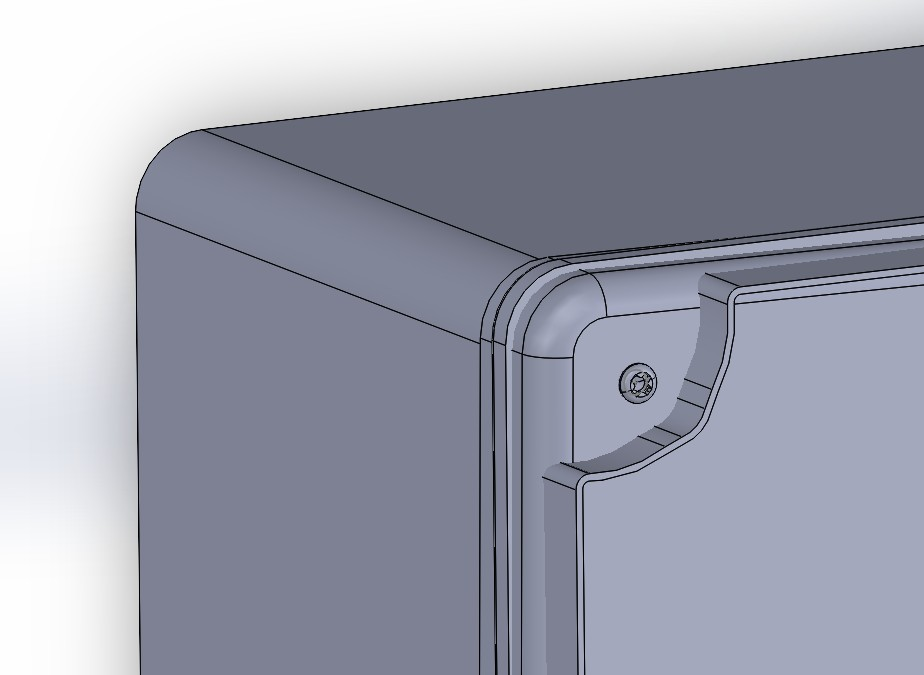
\includegraphics[width=\textwidth]{cad_uniones_caja.png}
        \caption{Unión de la tapa.}
    \end{subfigure}\\[6pt]
    \begin{subfigure}[b]{0.3\textwidth}
        \centering
        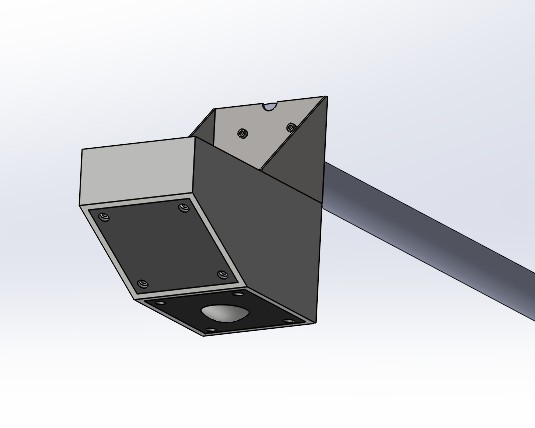
\includegraphics[width=\textwidth]{cad_soporte.png}
        \caption{Soporte del ultrasónico.}
    \end{subfigure}\hfill
    \begin{subfigure}[b]{0.3\textwidth}
        \centering
        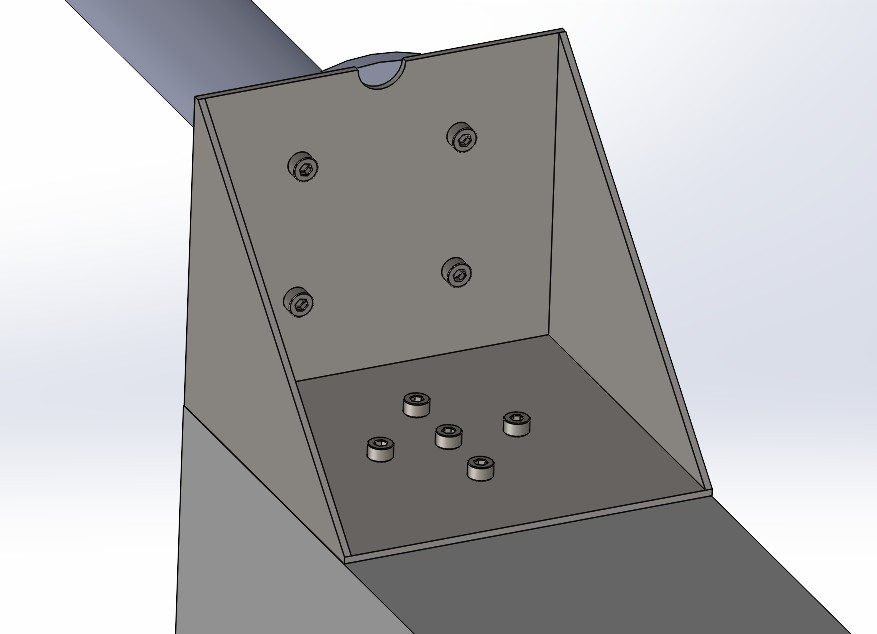
\includegraphics[width=\textwidth]{cad_uniones_soporte.png}
        \caption{Uniones del soporte.}
    \end{subfigure}\hfill
    \begin{subfigure}[b]{0.3\textwidth}
        \centering
        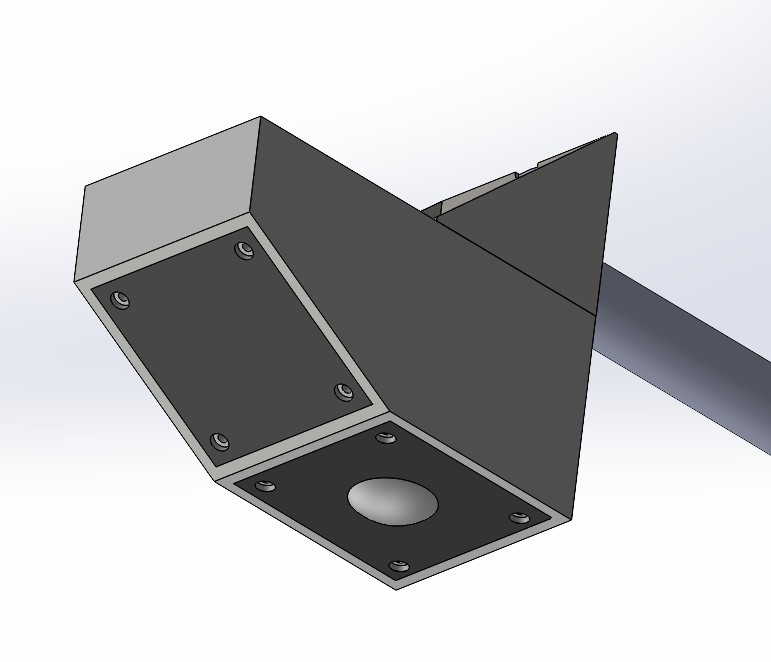
\includegraphics[width=\textwidth]{cad_render_inferior.png}
        \caption{Vista inferior.}
    \end{subfigure}
    \caption{Modelos CAD del primer parcial.}
\end{figure}

\begin{table}[H]
    \centering
    \small
    \caption{Elementos mecánicos.}
    \begin{tabularx}{\textwidth}{>{\raggedright\arraybackslash}p{3.4cm}L>{\raggedright\arraybackslash}p{3.3cm}}
        \toprule
        \textbf{Elemento} & \textbf{Función} & \textbf{Material / origen} \\
        \midrule
        Gabinete & Aloja PCB, UPS, módem y conexiones; tapa desmontable. &
            Comercial, plástico \\
        Soporte orientable (\emph{pico de pato}) & Sostiene el radar y permite
            nivelarlo. & Acero inoxidable, kit \\
        Placa adaptadora & Fija el soporte a un poste o caño (110 $\times$ 93
            mm, agujeros de 7 mm). & Acero inoxidable, kit \\
        Abrazaderas (3) & Sujetan la placa al poste. & Acero inoxidable, kit \\
        Cuerpo del radar & 159,5 $\times$ 95 $\times$ 99 mm; cara superior
            plana con nivel de burbuja. & Aluminio, comercial \\
        Fijaciones & Unión desmontable de las piezas. & Tornillería \\
        \bottomrule
    \end{tabularx}
\end{table}

\subsection{Montaje del radar en el banco de laboratorio}

El radar se montó con su soporte orientable en el extremo de un
\textbf{perfil metálico ranurado} en voladizo, fijado a una base de madera
sobre la mesa. Una varilla roscada une el perfil con el soporte y permite
ajustar la altura. Debajo se ubica el balde con agua. La PCB y la UPS quedan
sobre la misma base, como estarían dentro del gabinete.

\begin{figure}[!htbp]
    \centering
    \begin{subfigure}[b]{0.36\textwidth}
        \centering
        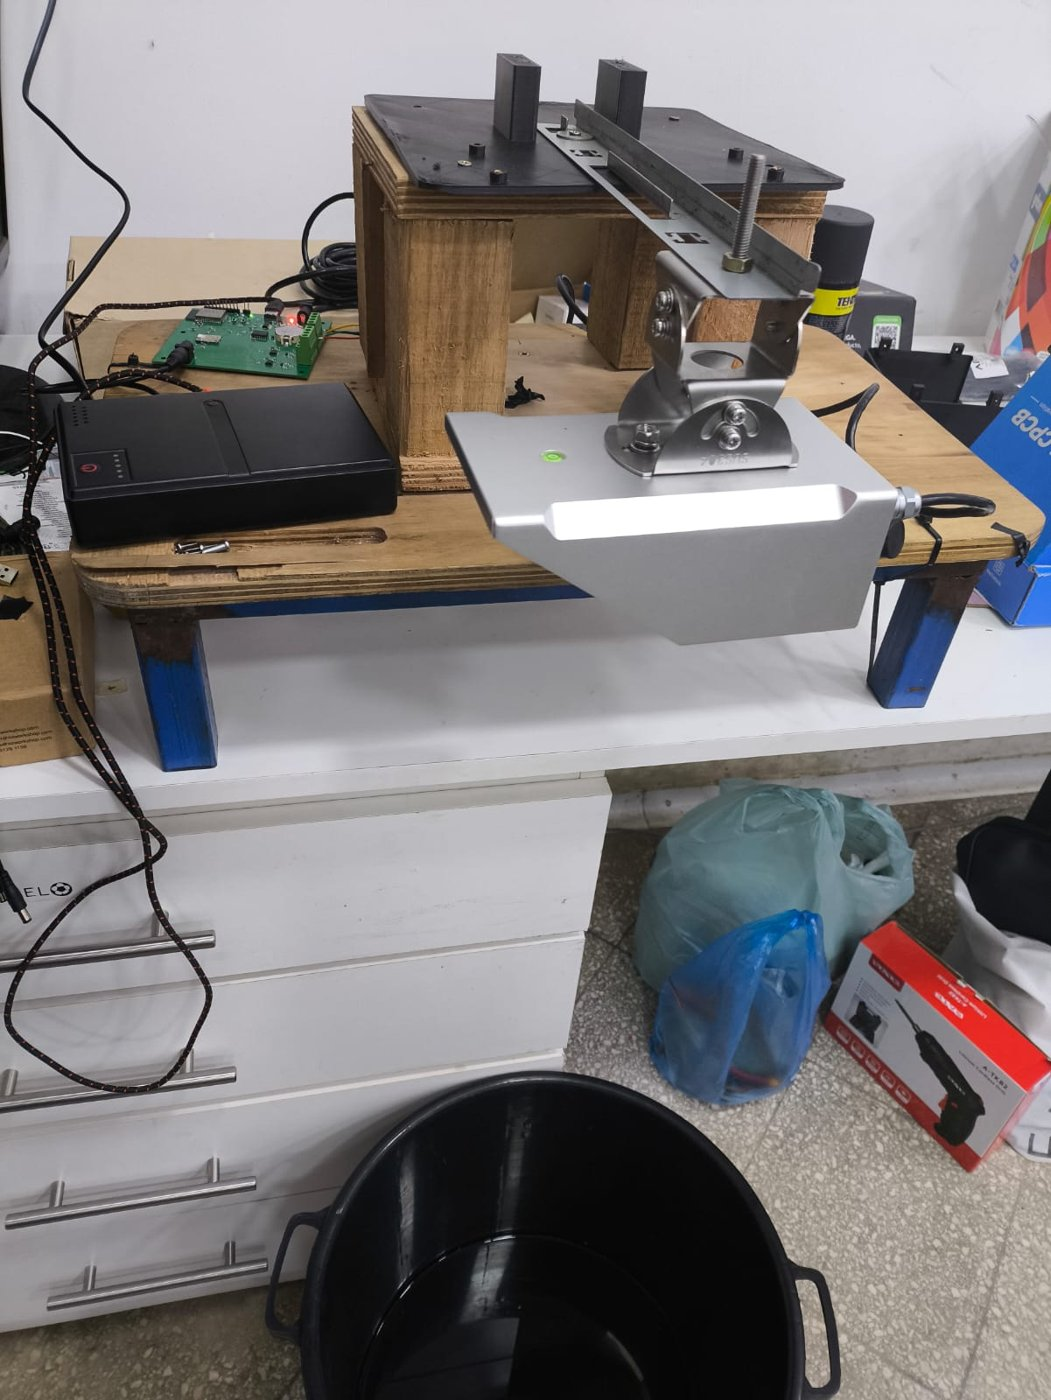
\includegraphics[height=6.5cm]{banco_lateral.jpg}
        \caption{Banco con el balde.}
    \end{subfigure}\hfill
    \begin{subfigure}[b]{0.6\textwidth}
        \centering
        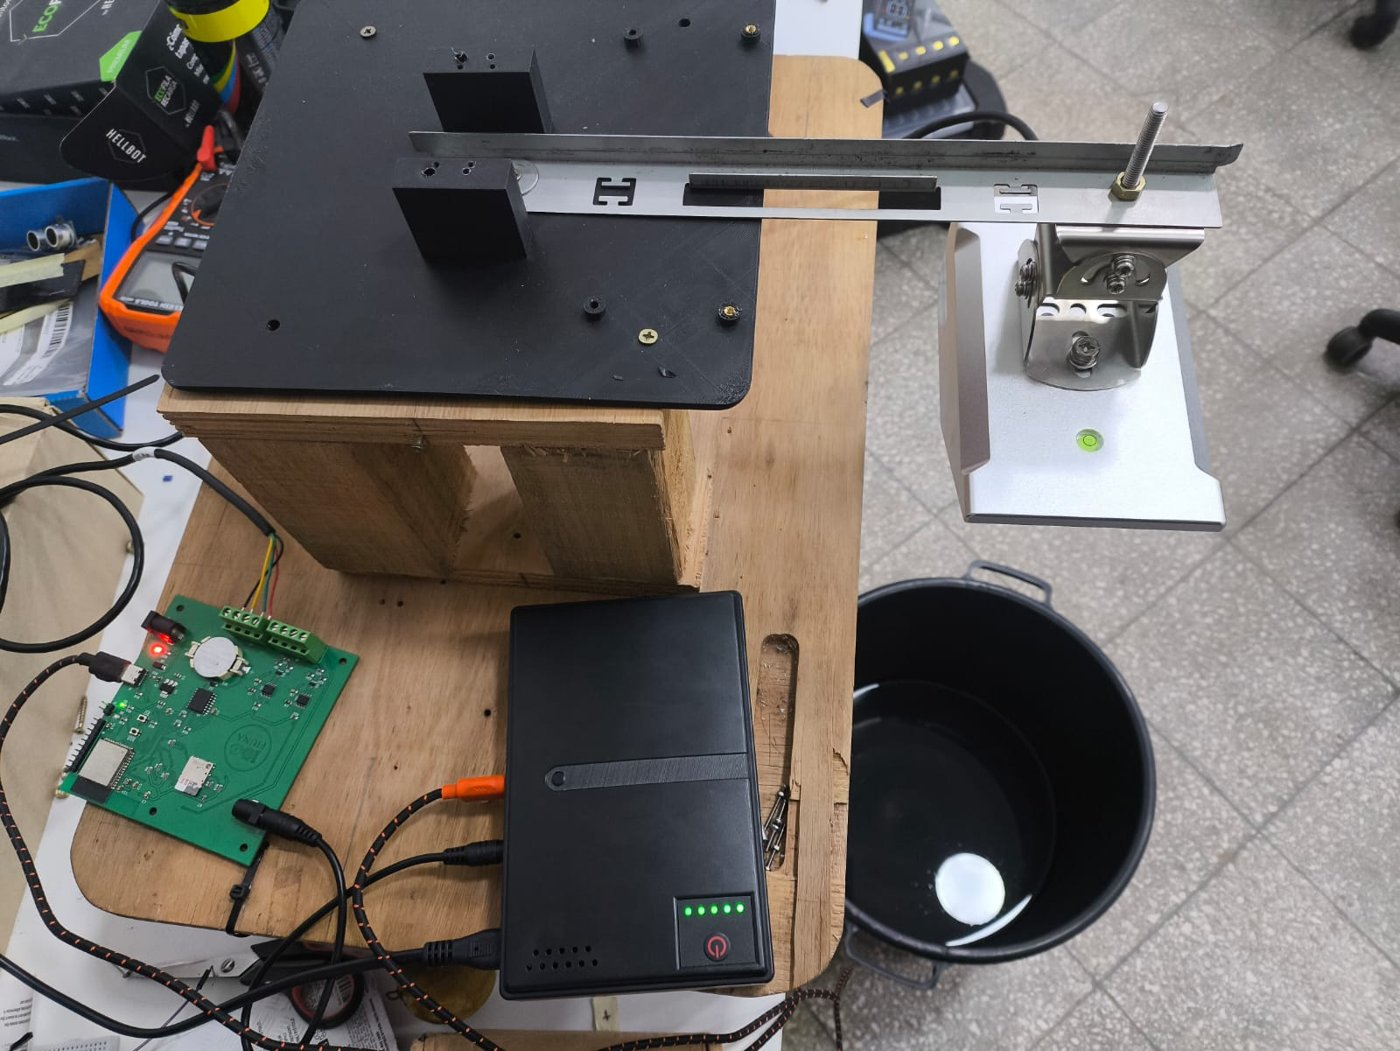
\includegraphics[height=6.5cm]{banco_superior.jpg}
        \caption{Vista superior: PCB, UPS, perfil y radar.}
    \end{subfigure}
    \caption{Banco de laboratorio.}
\end{figure}

\begin{figure}[!htbp]
    \centering
    \resizebox{0.85\textwidth}{!}{% Esquema del banco de laboratorio (vista lateral, sin escala)
\begin{tikzpicture}[
    cota/.style={<->, >=Stealth, gray!50!black},
    rot/.style={font=\footnotesize, align=center}
]
    % Piso
    \fill[gray!15] (-1,0) rectangle (10.5,-0.25);
    \draw[gray!60] (-1,0) -- (10.5,0);

    % Mesa y base de madera
    \fill[gray!30] (-0.5,3.0) rectangle (4.2,3.2);
    \draw[gray!60, thick] (0,0) -- (0,3.0) (3.8,0) -- (3.8,3.0);
    \fill[brown!45] (0.2,3.2) rectangle (3.9,3.45);
    \fill[brown!55] (0.9,3.45) rectangle (2.8,4.6);
    \fill[gray!80!black] (0.6,4.6) rectangle (3.4,4.72);
    \node[rot] at (1.85,4.05) {\color{white}base};

    % Electrónica sobre la base
    \fill[green!45!black] (0.25,3.45) rectangle (0.85,3.6);
    \node[rot, anchor=south] at (0.3,3.7) {PCB};
    \fill[black!80] (2.9,3.45) rectangle (3.85,3.75);
    \node[rot, anchor=south] at (3.4,3.8) {UPS};

    % Perfil en voladizo
    \fill[gray!60] (2.4,4.72) rectangle (7.6,4.86);
    \node[rot, above] at (4.6,4.86) {perfil metálico ranurado};
    \draw[gray!50!black, very thick] (7.1,4.0) -- (7.1,5.3);
    \node[rot, right] at (7.2,5.35) {varilla roscada};

    % Soporte pico de pato + radar
    \fill[gray!45] (6.8,3.65) -- (7.4,3.65) -- (7.3,4.0) -- (6.9,4.0) -- cycle;
    \fill[gray!35, draw=gray!60!black] (6.0,3.15) rectangle (8.2,3.65);
    \fill[gray!35, draw=gray!60!black] (8.2,3.65) -- (8.2,3.15) -- (8.7,3.15) -- cycle;
    \fill[green!60] (6.4,3.65) circle (2pt);
    \node[rot, right] at (8.7,3.55) {radar FM02B\\(burbuja arriba)};

    % Balde con agua
    \fill[cyan!20] (5.85,0.05) rectangle (8.35,0.95);
    \draw[very thick] (5.75,1.5) -- (5.85,0) -- (8.35,0) -- (8.45,1.5);
    \node[rot] at (7.1,0.45) {agua};
    \node[rot, right] at (8.45,0.35) {balde $\approx$ 30 cm};

    % Haz 14°
    \fill[radar!20, opacity=0.8] (7.1,3.15) -- (6.67,0.95) -- (7.53,0.95) -- cycle;
    \draw[radar, thick] (6.67,0.95) -- (7.1,3.15) -- (7.53,0.95);
    \node[rot, radar] at (7.1,2.05) {14°};

    % Cotas
    \draw[cota] (5.4,3.15) -- node[rot, left] {$d$ radar\\(registro \texttt{0x0001})} (5.4,0.95);
    \draw[cota] (9.6,3.15) -- node[rot, right] {$d$ cinta\\(referencia)} (9.6,0.95);
    \draw[gray!50, densely dotted] (8.2,3.15) -- (9.8,3.15) (7.53,0.95) -- (9.8,0.95);
    \draw[gray!50, densely dotted] (5.2,3.15) -- (6.0,3.15) (5.2,0.95) -- (5.85,0.95);
\end{tikzpicture}
}
    \caption{Esquema del banco (sin escala). La distancia del radar se
    compara con la medida con cinta métrica.}
\end{figure}

Criterios de montaje tomados del manual~\cite{fm02b_montaje}:

\begin{itemize}
    \item \textbf{Antena perpendicular al agua.} Se niveló con el nivel de
        burbuja de la cara superior del radar, en los dos ejes, ajustando el
        soporte orientable.
    \item \textbf{Haz libre.} El radar se centra sobre el balde y a menos de
        1,2~m del agua; se retiraron objetos metálicos del cono del haz.
    \item \textbf{Cable.} Sin peso colgando del conector y con un bucle en
        ``U'' por debajo de la ficha, para que el agua no escurra hacia ella.
\end{itemize}

\begin{figure}[!htbp]
    \centering
    \begin{subfigure}[b]{0.28\textwidth}
        \centering
        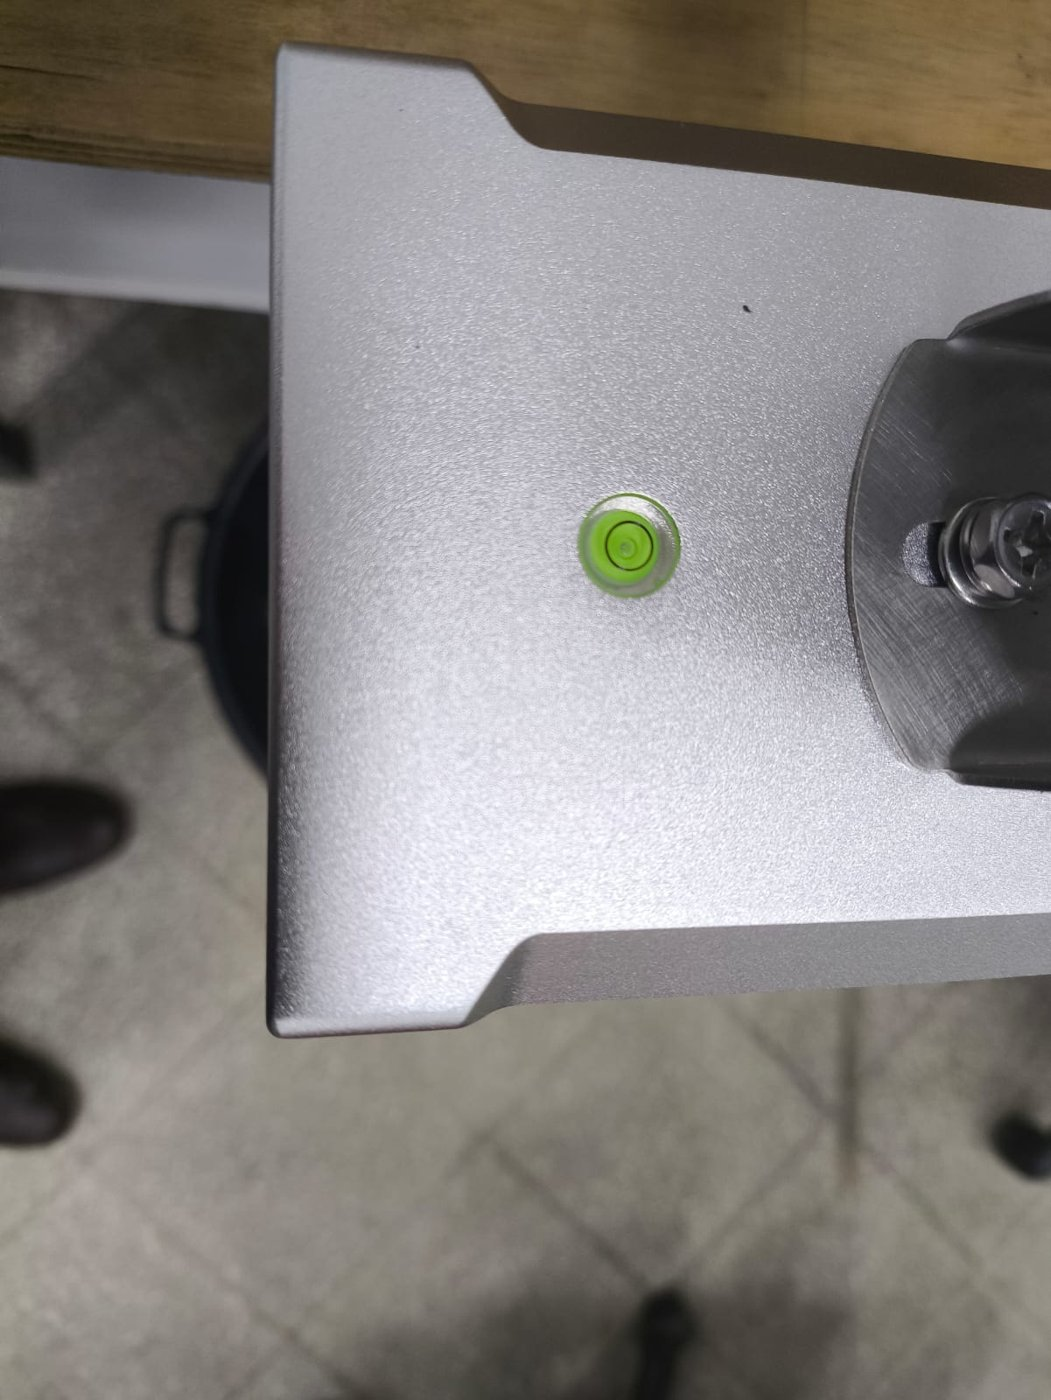
\includegraphics[height=4.6cm]{radar_nivelado.jpg}
        \caption{Burbuja centrada.}
    \end{subfigure}\hfill
    \begin{subfigure}[b]{0.28\textwidth}
        \centering
        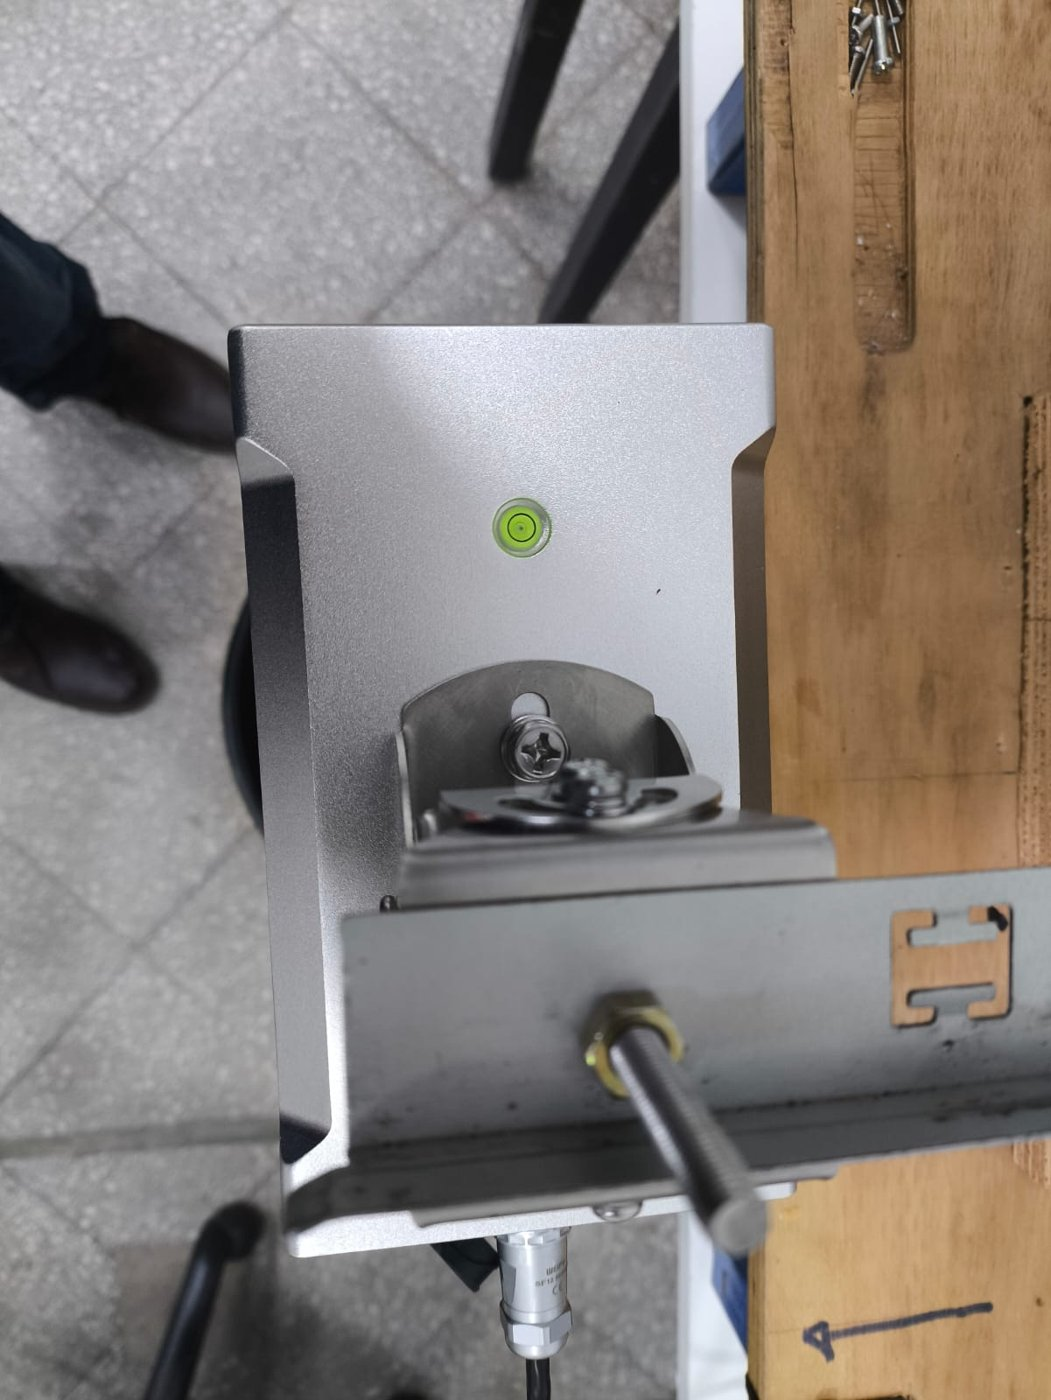
\includegraphics[height=4.6cm]{radar_nivelado2.jpg}
        \caption{Soporte orientable.}
    \end{subfigure}\hfill
    \begin{subfigure}[b]{0.4\textwidth}
        \centering
        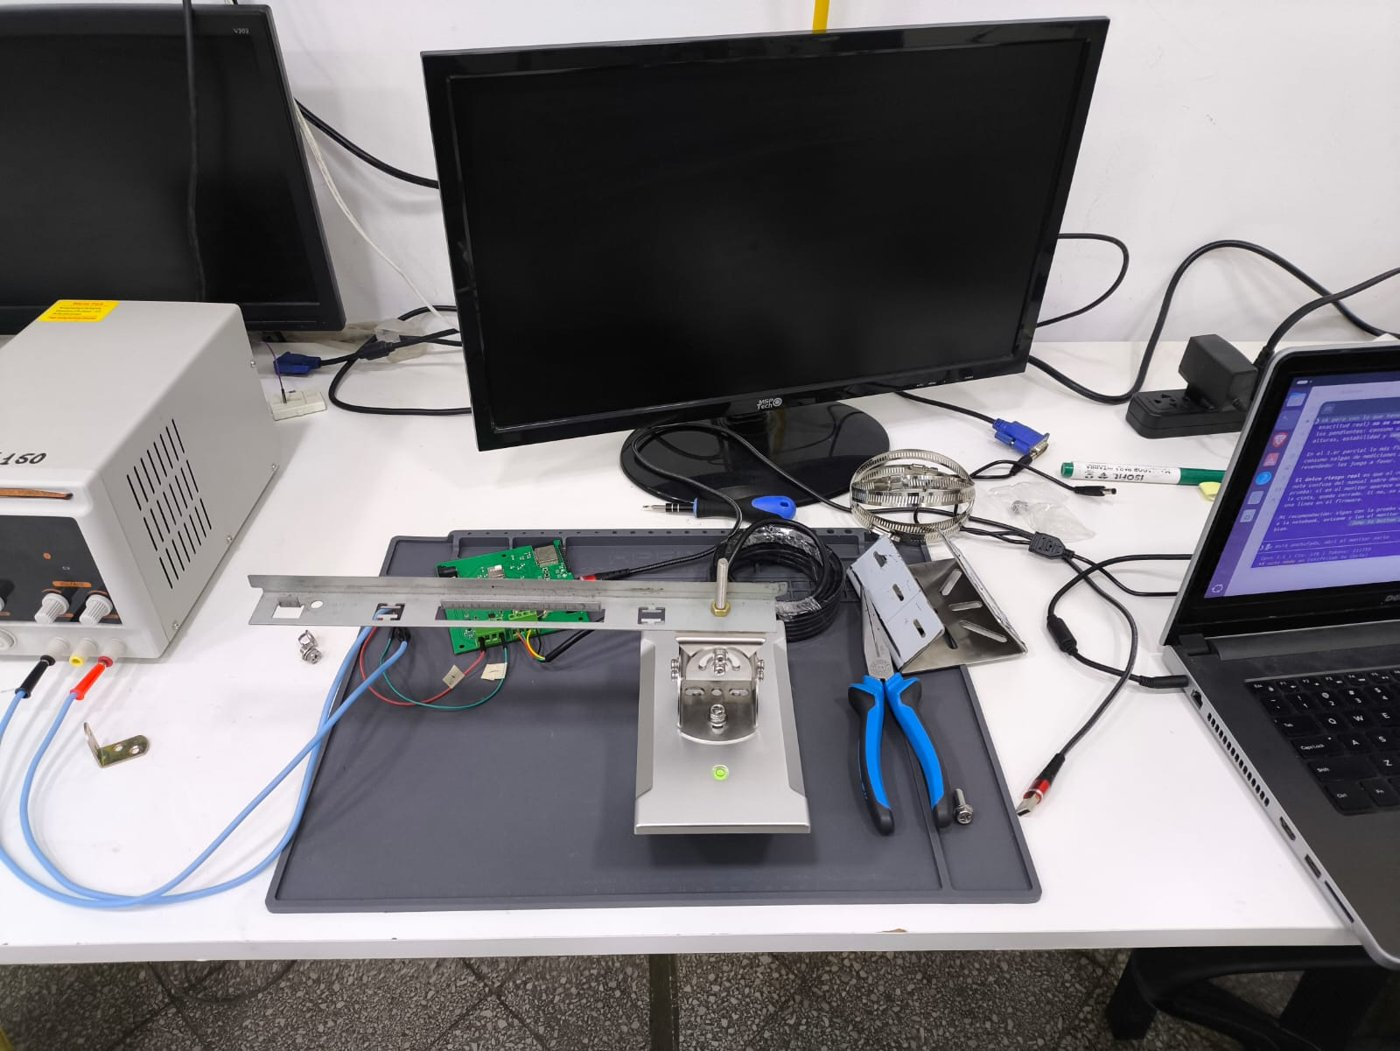
\includegraphics[height=4.6cm]{perfil_improvisado.jpg}
        \caption{Primer armado del perfil.}
    \end{subfigure}
    \caption{Nivelación del radar y armado del perfil.}
\end{figure}

\subsection{Planos}

Los planos acotados del primer parcial se incluyen al final, en el
anexo~\ref{sec:planos}.

% ======================================================
% 10. ENSAYOS
% ======================================================
\seccion{Ensayos en banco de laboratorio}

Todos los ensayos se hicieron en el laboratorio. Las pruebas de Proyecto~3
(9 meses de datos del sensor ultrasónico) sirven de línea de base; aquí se
cuantifica.

\begin{table}[H]
    \centering
    \small
    \caption{Plan de ensayos y avance.}
    \begin{tabularx}{\textwidth}{>{\raggedright\arraybackslash}p{2.3cm}L>{\raggedright\arraybackslash}p{2.1cm}L}
        \toprule
        \textbf{Ensayo} & \textbf{Cómo} & \textbf{Umbral} & \textbf{Avance} \\
        \midrule
        Comunicación & Lecturas del radar con el firmware. & Sin errores
            de CRC & \REAL \\
        Exactitud & $\geq$ 4 alturas $\times$ 10 lecturas sobre agua, contra
            cinta métrica. & $\leq\pm$10 mm & \CURSO \\
        Consumo & Corriente de cada módulo con fuente de laboratorio y
            medidor USB. & Se informa & \CURSO\ (radar listo) \\
        Cortes de red & $\geq$ 10 cortes del router, cortos y largos. & 0
            perdidos, 0 duplicados & \CURSO\ (1 de 10) \\
        Cortes de energía & $\geq$ 10, incluso durante la escritura. & 0
            perdidos, 0 duplicados & \CURSO \\
        Disponibilidad & 7 días continuos a 5 min. & $\geq$ 95\,\% & \CURSO \\
        Autonomía & Corte de red eléctrica con la UPS cargada. & Se informa &
            \CURSO \\
        Velocidad & Agua en movimiento en un canal. & $\pm$0,01 m/s (ficha) &
            \ESPERA \\
        \bottomrule
    \end{tabularx}
\end{table}

\subsection{Comunicación con el radar}

\begin{resultado}{Resultado}
El radar respondió a la primera con el firmware: 115\,200 baudios, dirección
1, sin invertir A/B y \textbf{sin errores de CRC}. El registro \texttt{0x0001}
quedó confirmado como distancia en milímetros: \textbf{0,197~m del radar
contra 19,7~cm con cinta}, apuntando a una superficie sólida.
\end{resultado}

La señal sobre superficies sólidas fue de 15 a 18~dB, por debajo de los 30~dB
que el manual considera buena. Es esperable con la potencia de emisión en el
mínimo (7); si sobre el agua sigue baja, se sube la potencia (7 $\to$ 3
$\to$ 0) antes de tocar la calibración.

\subsection{Exactitud del nivel sobre agua}
\label{sec:exactitud}

\textbf{Procedimiento.} Con el firmware en modo banco y el radar nivelado sobre
el balde: (1) se fija una altura de agua; (2) se mide con cinta métrica la
distancia desde la cara inferior del radar hasta la superficie; (3) se toman
10 lecturas del radar; (4) se repite para al menos 4 alturas. Se informa el
error medio, el máximo y la señal.

\begin{table}[H]
    \centering
    \small
    \caption{Distancia del radar frente a la cinta métrica (en mm; señal en dB).}
    \begin{tabular}{cccccc}
        \toprule
        \textbf{Altura} & \textbf{Cinta} & \textbf{Radar (media)} &
            \textbf{Error medio} & \textbf{Error máx.} & \textbf{Señal} \\
        \midrule
        1 & \completar{} & \completar{} & \completar{} & \completar{} & \completar{} \\
        2 & \completar{} & \completar{} & \completar{} & \completar{} & \completar{} \\
        3 & \completar{} & \completar{} & \completar{} & \completar{} & \completar{} \\
        4 & \completar{} & \completar{} & \completar{} & \completar{} & \completar{} \\
        \bottomrule
    \end{tabular}
\end{table}

\completar{Conclusión del ensayo: ¿error $\leq\pm$10 mm? ¿error constante
(corregir la calibración de $-46$ mm) o variable?}

\begin{figure}[!htbp]
    \centering
    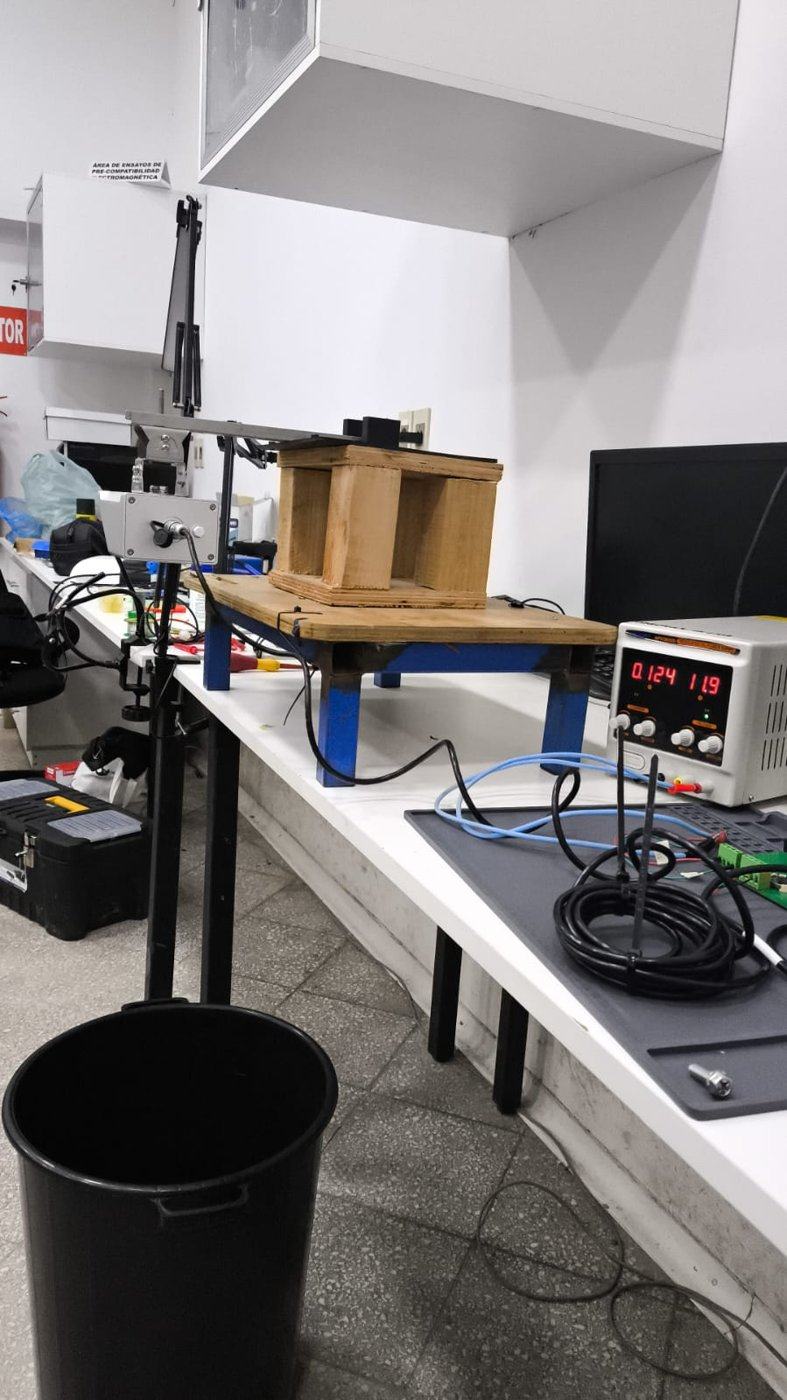
\includegraphics[height=7cm]{banco_balde.jpg}\hspace{1cm}
    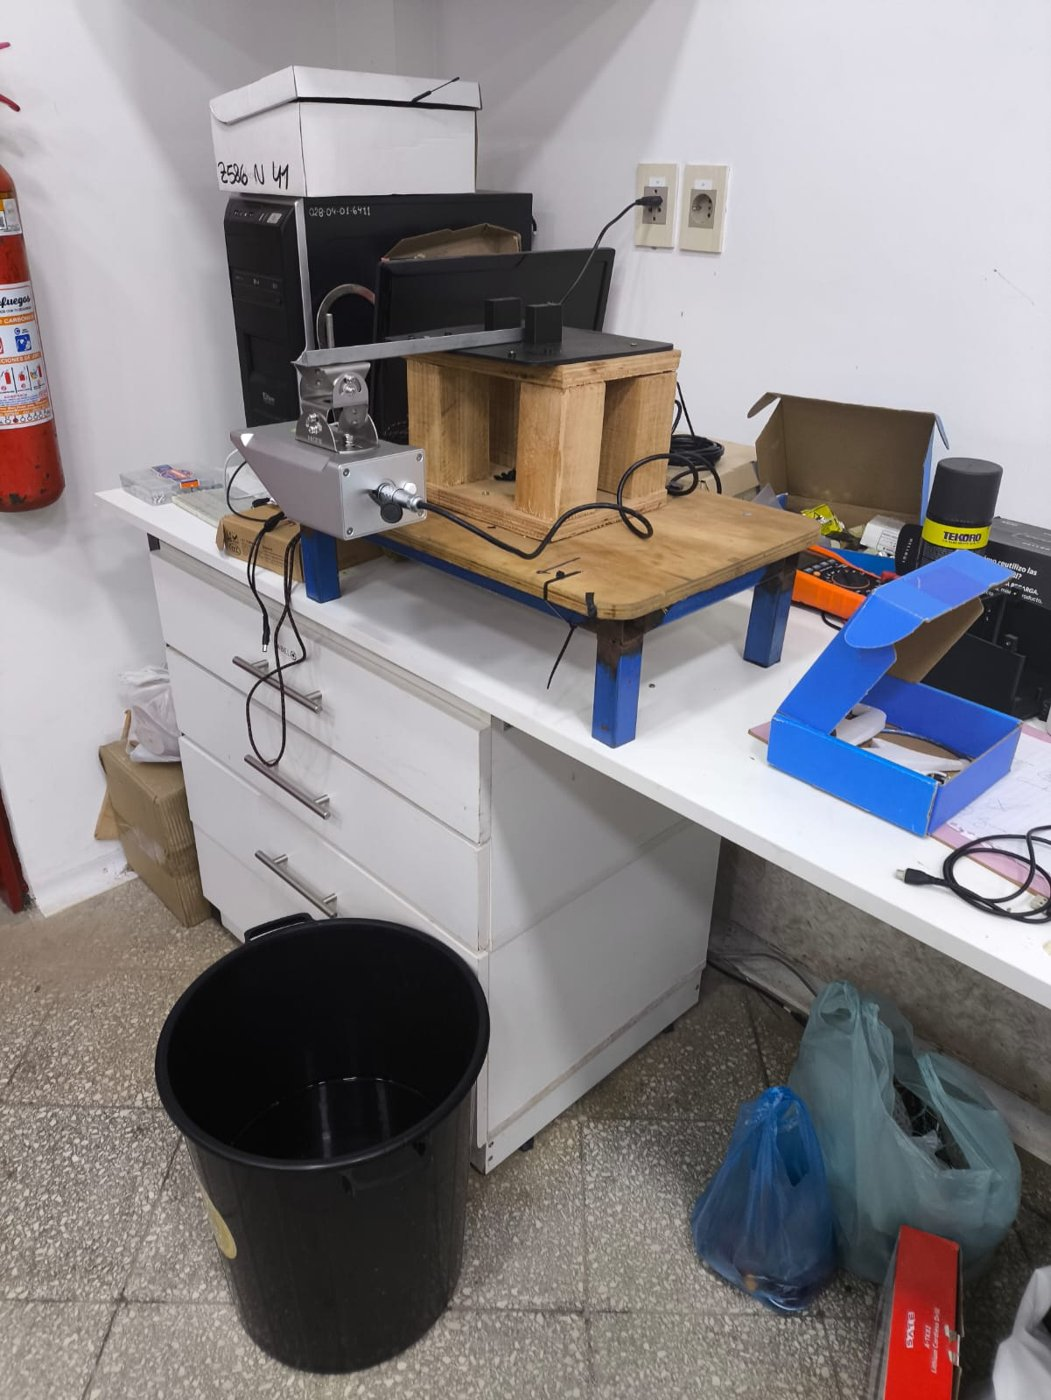
\includegraphics[height=7cm]{banco_general.jpg}
    \caption{Radar sobre el balde con agua durante el ensayo de nivel.}
\end{figure}

\subsection{Consumo}

El radar se alimentó con la fuente de laboratorio a 12~V para leer su
corriente.

\begin{figure}[!htbp]
    \centering
    \begin{minipage}[c]{0.5\textwidth}
        \centering
        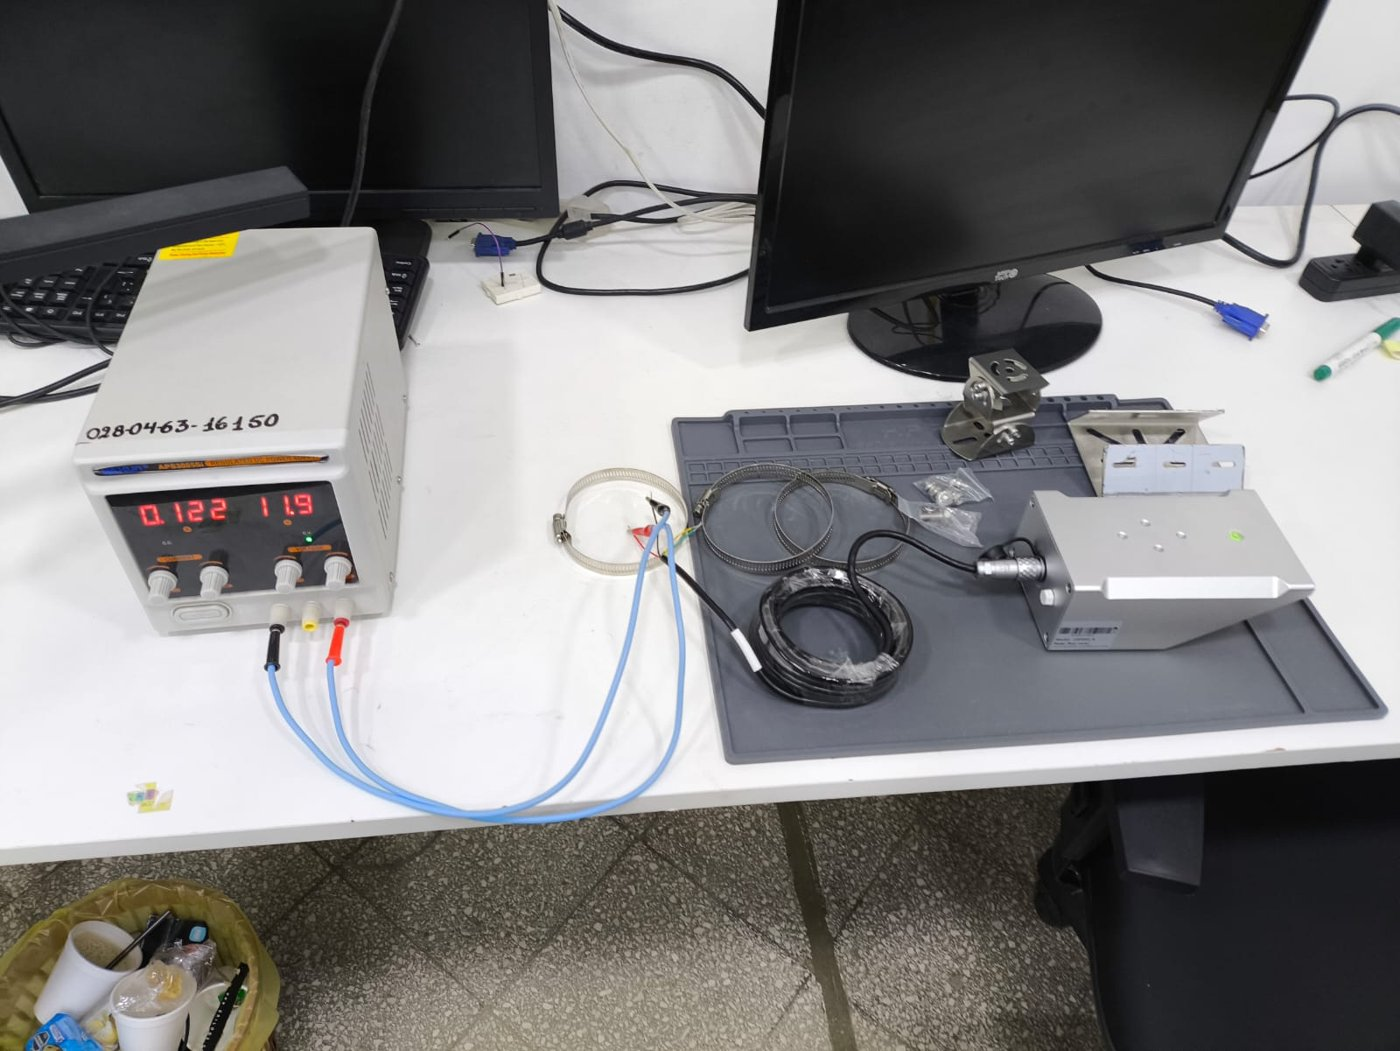
\includegraphics[width=\textwidth]{consumo_radar.jpg}
    \end{minipage}\hfill
    \begin{minipage}[c]{0.46\textwidth}
        \begin{resultado}{Resultado}
            \textbf{126 mA a 12 V ($\approx$1,5 W)}, dentro de los 130--160 mA
            de la ficha. El radar \textbf{no tiene modo de reposo}: consume
            siempre lo mismo, mida o no.
        \end{resultado}
    \end{minipage}
    \caption{Medición de la corriente del radar con la fuente de laboratorio.}
\end{figure}

Con ese dato se rehace el balance de energía. La parte del ESP32 se mide con un
medidor USB; mientras tanto se usa un valor estimado.

\begin{table}[H]
    \centering
    \small
    \caption{Balance de energía del modo WiFi.}
    \begin{tabular}{lrl}
        \toprule
        \textbf{Consumidor} & \textbf{Potencia} & \textbf{Origen} \\
        \midrule
        Radar FM02B & 1,5 W & medido \\
        ESP32-S3 + WiFi + periféricos & 0,5--1 W & estimado, a medir \\
        \midrule
        Total & 2--2,5 W & \\
        Batería UPS (16\,000 mAh a 3,7 V, 80\,\% de eficiencia) & $\approx$ 47 Wh & \\
        \textbf{Autonomía estimada} & \textbf{19--23 h} & a confirmar con descarga \\
        \bottomrule
    \end{tabular}
\end{table}

En modo módem se suma el consumo del DTU, que se medirá al reintegrarlo.

\subsection{Corte de red}

Con la estación midiendo cada 1~min, se apagó el router durante unos 7 minutos.

\begin{figure}[!htbp]
    \centering
    \resizebox{0.9\textwidth}{!}{% Corte de red n.o 1 (19/11/2026, intervalo de 1 min): línea de tiempo
% Escala: 1 min = 1.15 cm, origen 22:14:00
\begin{tikzpicture}[x=1.15cm,
    rot/.style={font=\scriptsize, align=center}]
    % WiFi caído: 22:15:29 -> 22:22:31
    \fill[red!12] (1.483,-0.35) rectangle (8.517,0.35);
    \node[rot, text=red!60!black] at (5,0.6) {WiFi caído (router apagado) -- 7 min 2 s};
    % Vaciado de la cola: 22:22:31 -> 22:24:07
    \fill[agua!25] (8.517,-0.35) rectangle (10.117,0.35);
    \node[rot, text=agua!50!black, anchor=west] at (8.5,-0.95) {reenvío FIFO: 1 min 36 s};

    \draw[-{Stealth}, thick] (0,0) -- (11,0);
    \foreach \m in {0,...,10} {
        \pgfmathtruncatemacro{\mm}{14+\m}
        \draw (\m,-0.08) -- (\m,0.08);
        \node[rot, below] at (\m,-0.4) {22:\mm};
    }
    % Mediciones
    \foreach \m in {0,1,9,10} \fill[agua!70!black] (\m,0) circle (3pt);
    \foreach \m in {2,...,8} {
        \fill[red!70!black] (\m,0) circle (3pt);
    }
    \node[rot, text=red!60!black] at (5,-1.45) {7 mediciones (22:16 a 22:22) $\to$ \texttt{temp.csv}};
    \node[rot, anchor=west] at (0,1.15) {%
        \tikz\fill[agua!70!black] (0,0) circle (3pt); enviada en el momento \quad
        \tikz\fill[red!70!black] (0,0) circle (3pt); guardada como pendiente};
\end{tikzpicture}
}
    \caption{Corte de red n.º 1 (19/11/2026).}
\end{figure}

\begin{resultado}{Resultado del corte n.º 1}
WiFi caído de 22:15:29 a 22:22:31. Las \textbf{7 mediciones} de ese lapso
quedaron en la cola y se reenviaron en orden: \textbf{7 recuperadas, 0
perdidas, 0 duplicadas} (verificado en la base de datos). La cola quedó vacía
\textbf{1~min 36~s} después de volver la red.
\end{resultado}

Faltan 9 cortes de distintos tipos (sin internet pero con WiFi, cortos de menos
de 1~min y largos de más de 10~min).

\subsection{Funcionamiento continuo}

Desde el 20/11/2026 a las 00:30 la estación funciona sola, alimentada sin
computadora, midiendo cada 5 minutos y enviando por WiFi (RSSI $-43$~dBm). Con
estos datos se calcula la disponibilidad: datos recibidos frente a esperados,
huecos y duplicados.

\begin{table}[H]
    \centering
    \small
    \caption{Disponibilidad del período de funcionamiento continuo.}
    \begin{tabular}{lc}
        \toprule
        Período & \completar{desde 20/11 00:30 hasta ...} \\
        Datos esperados (1 cada 5 min) & \completar{} \\
        Datos recibidos en el servidor & \completar{} \\
        Disponibilidad & \completar{\%} \\
        Duplicados & \completar{} \\
        \bottomrule
    \end{tabular}
\end{table}

\subsection{Velocidad superficial}

\ESPERA\ El firmware ya lee la velocidad (registro \texttt{0x01F4}) y la guarda
en la microSD; en el banco da 0,000~m/s, lo esperable con el agua quieta. Para
validarla hace falta agua en movimiento: un canal o un tramo de arroyo. En el
laboratorio no se puede montar un canal, así que este ensayo queda en espera
hasta conseguir uno.

\subsection{Problemas encontrados}

\begin{table}[H]
    \centering
    \small
    \caption{Problemas detectados durante los ensayos y solución aplicada.}
    \begin{tabularx}{\textwidth}{LL}
        \toprule
        \textbf{Problema} & \textbf{Solución} \\
        \midrule
        El RTC estaba en el año 2000 y se enviaron datos con esa fecha (y
            $-1$ porque el radar no estaba conectado). & Hora por NTP al
            arrancar; no se mide sin hora válida; se descartan los pendientes
            con fecha inválida. \\
        La tabla del manual dice 9600 baudios de fábrica. & Se leyó la
            unidad por Bluetooth: 115\,200. \\
        No hay hoja de datos oficial publicada; los documentos llaman al
            equipo LDFM01, LDFM02\_B o LDFM04\_B. & Se usan los tres
            documentos del vendedor y se identifica la unidad por serie y
            firmware. \\
        Señal de 15--18 dB (el manual pide $>$ 30). & Potencia de emisión
            en el mínimo; se ajusta según el ensayo con agua. \\
        El script del servidor acepta solo dos campos. & id, velocidad,
            señal y estado van a la microSD; estado calculado en la base de
            datos. \\
        \bottomrule
    \end{tabularx}
\end{table}

\begin{figure}[!htbp]
    \centering
    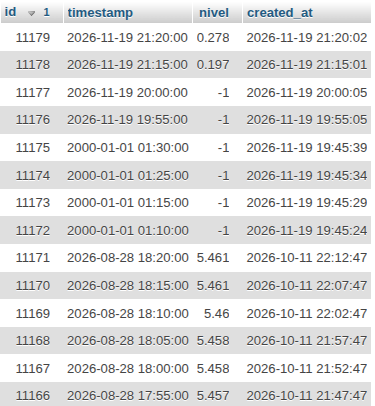
\includegraphics[width=0.55\textwidth]{bd_registros_banco.png}
    \caption{Registros del servidor durante las primeras pruebas: datos con
    fecha del año 2000 y $-1$ (antes del NTP), y las primeras distancias del
    radar (0,197 m y 0,278 m).}
\end{figure}

\subsection{Videos}

Los videos de los ensayos se publican en YouTube: \completar{enlace}.

% ======================================================
% 11. INTERFAZ
% ======================================================
\seccion{Base de datos e interfaz de usuario}

\subsection{Interfaces existentes}

Durante Proyecto~3 los datos se visualizaron en un panel de
\textbf{Grafana}~\cite{grafana}, con nivel, precipitación, estado de
actualización y mapa. El grupo de investigación publica además la web
\textbf{MburicaoCastAI}, con monitoreo y predicción de crecidas. Ambas son
trabajos externos a este proyecto académico y aquí solo se citan.

\begin{figure}[!htbp]
    \centering
    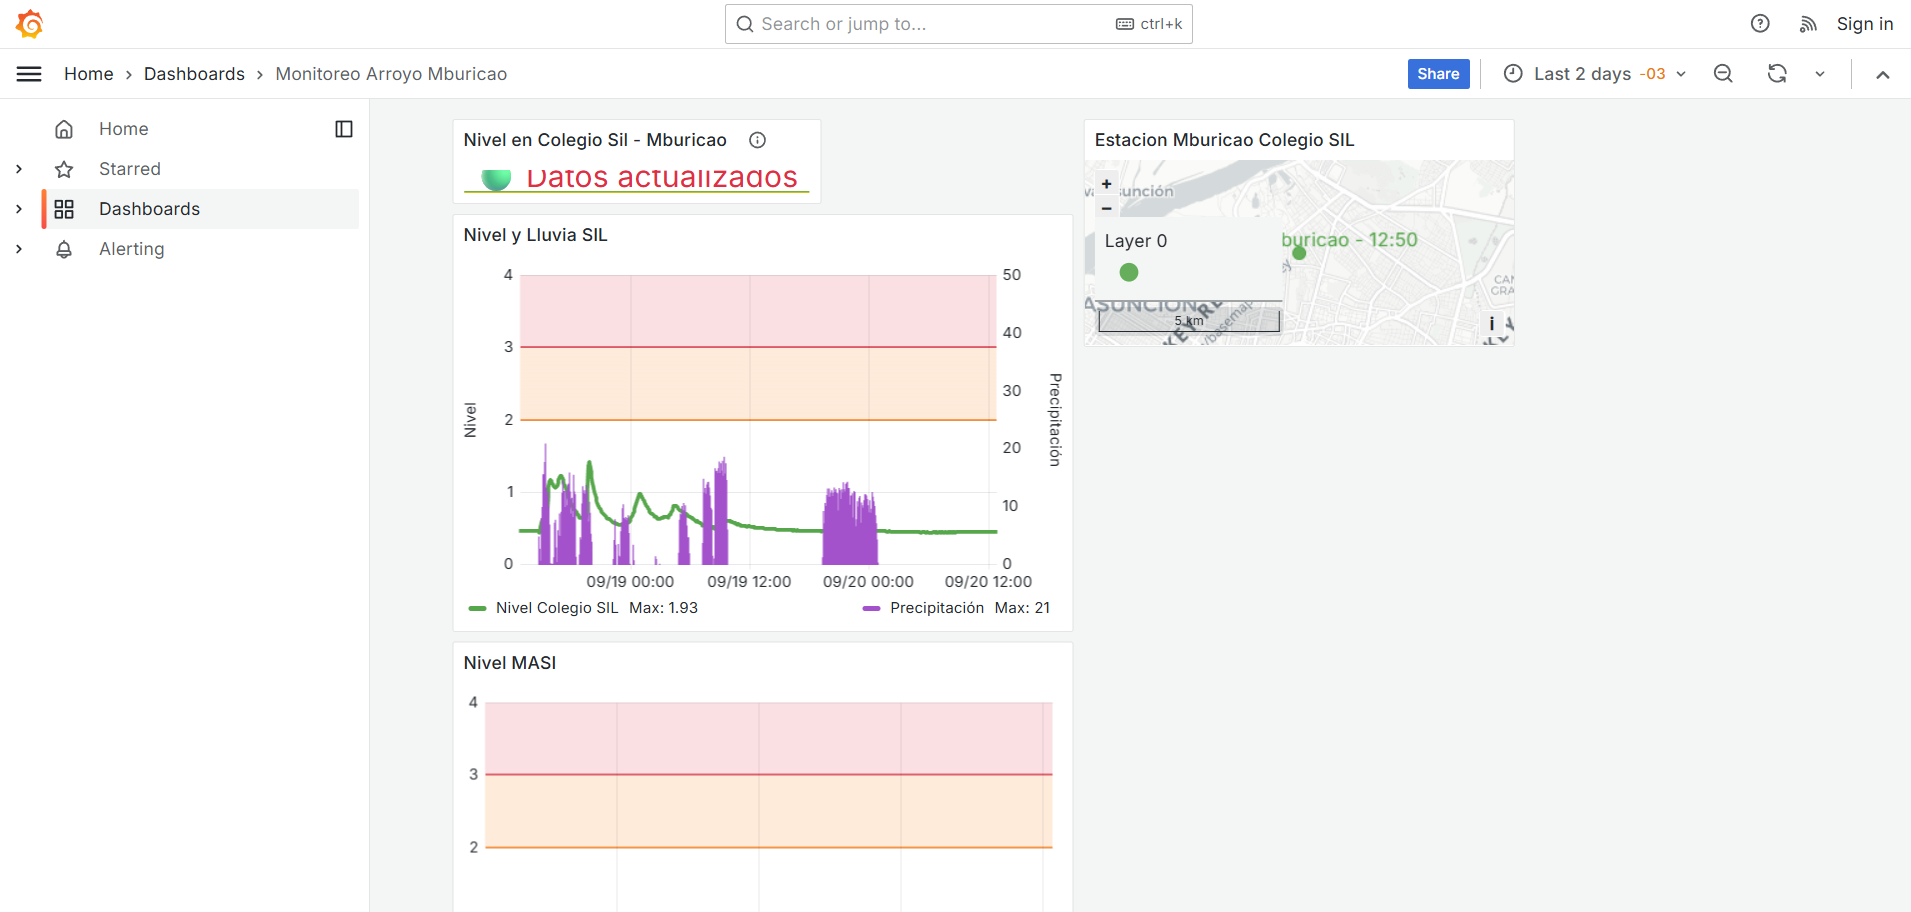
\includegraphics[width=0.49\textwidth]{grafana.png}\hfill
    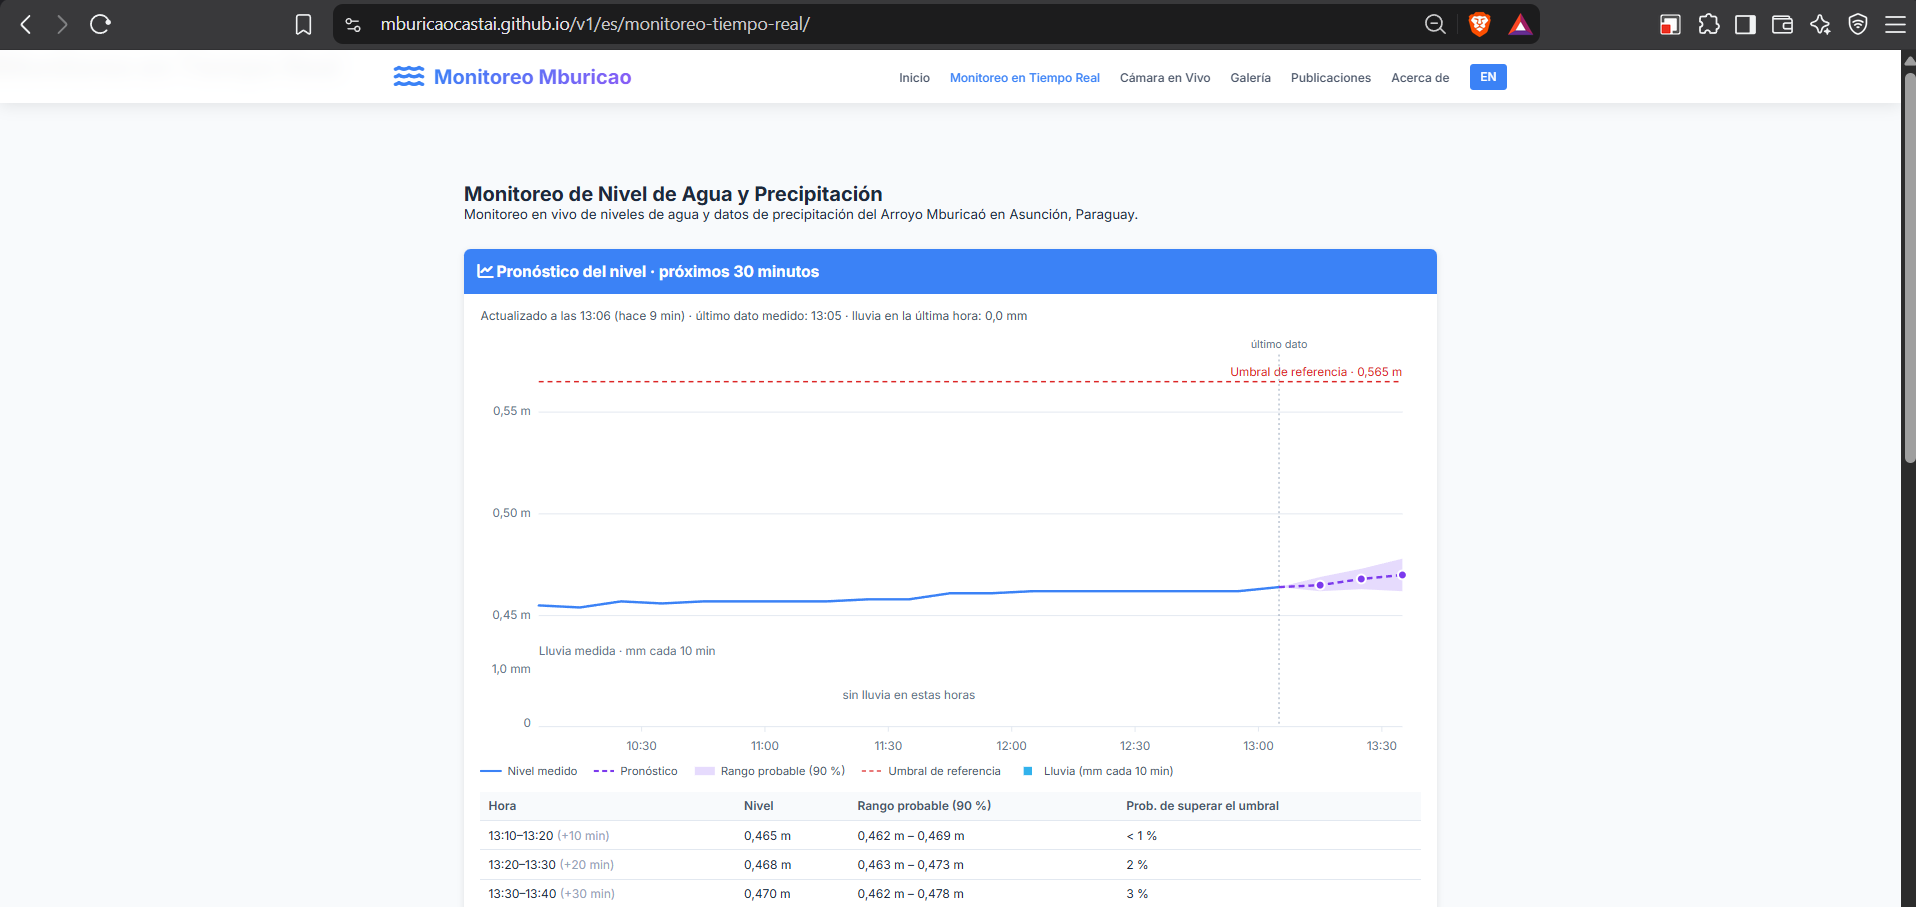
\includegraphics[width=0.49\textwidth]{web_mburicao.png}
    \caption{Panel de Grafana (izq.) y web MburicaoCastAI (der.).}
\end{figure}

\subsection{Estado del dato en la base de datos}

Como el servidor no se puede modificar, el estado se calcula en la base de
datos, donde el equipo sí tiene acceso:

\begin{itemize}
    \item \textbf{Columna \texttt{estado}} de cada registro:
        \texttt{FALLA\_SENSOR} si el valor es $-1$; \texttt{RECUPERADO} si llegó
        más de 2 minutos tarde (vino de la cola); si no, \texttt{OK}.
    \item \textbf{Vista de estado de la estación}: \texttt{EN LINEA} o
        \texttt{CAIDA} si pasan más de 15 minutos (3 lecturas) sin datos.
\end{itemize}

Ambas funcionan y son la base de la web propia.

\subsection{Web propia}

\CURSO\ La web del equipo muestra los históricos, la antigüedad de la última
lectura, el estado del sensor y una alarma por umbral. Se prueba primero con
los datos históricos de Proyecto~3 y luego con los del radar.

\begin{figure}[!htbp]
    \centering
    \resizebox{0.85\textwidth}{!}{% Boceto de la web propia (valores ilustrativos)
\begin{tikzpicture}[
    tarjeta/.style={draw=gray!50, fill=white, rounded corners=3pt, minimum height=1.35cm, align=center, font=\small},
    rotulo/.style={font=\scriptsize, text=gray!60!black}
]
    % Ventana del navegador
    \draw[gray!60, fill=gray!5, rounded corners=5pt] (0,0) rectangle (13,7.6);
    \fill[gray!25, rounded corners=5pt] (0,7.0) rectangle (13,7.6);
    \fill[gray!25] (0,7.0) rectangle (13,7.2);
    \foreach \x in {0.3,0.6,0.9} \fill[gray!55] (\x,7.3) circle (0.08);
    \node[anchor=west, font=\small\bfseries] at (1.3,7.3) {Estación de nivel -- arroyo Mburicaó (datos abiertos)};

    % Alarma
    \draw[draw=orange!80!black, fill=orange!15, rounded corners=3pt] (0.4,6.15) rectangle (12.6,6.75);
    \node[font=\small, text=orange!50!black] at (6.5,6.45) {\textbf{Alarma:} el nivel superó el umbral configurado};

    % Tarjetas
    \node[tarjeta, minimum width=2.8cm] at (1.85,5.1) {{\scriptsize\color{gray!60!black} Nivel actual}\\{\Large\bfseries 0,52 m}};
    \node[tarjeta, minimum width=2.8cm] at (4.95,5.1) {{\scriptsize\color{gray!60!black} Velocidad}\\{\Large\bfseries 0,35 m/s}};
    \node[tarjeta, minimum width=2.8cm] at (8.05,5.1) {{\scriptsize\color{gray!60!black} Última lectura}\\{\bfseries hace 2 min}};
    \node[tarjeta, minimum width=2.8cm] at (11.15,5.1) {{\scriptsize\color{gray!60!black} Estado del sensor}\\{\bfseries\textcolor{agua!80!black}{$\bullet$ OK}}};

    % Gráfico de históricos
    \draw[gray!50, fill=white, rounded corners=3pt] (0.4,0.4) rectangle (12.6,4.1);
    \node[anchor=west, font=\footnotesize\bfseries] at (0.6,3.8) {Históricos};
    \node[anchor=east, rotulo] at (12.4,3.8) {24 h \quad 7 días \quad 30 días};
    \draw[gray!40] (1,0.8) -- (12.2,0.8);
    \draw[gray!40] (1,0.8) -- (1,3.4);
    \draw[radar, thick] plot[smooth] coordinates {(1,1.1) (2,1.15) (3,1.1) (4,1.2) (4.6,2.9) (5.1,1.5) (6,1.2) (7,1.15) (8,1.2) (8.6,2.3) (9.1,1.3) (10,1.15) (11,1.2) (12.2,1.15)};
    \draw[orange!80!black, dashed] (1,2.6) -- (12.2,2.6) node[above left, rotulo, text=orange!60!black] {umbral de alarma};
\end{tikzpicture}
}
    \caption{Diseño de la web propia (valores ilustrativos).}
\end{figure}

% ======================================================
% 12. COSTOS
% ======================================================
\seccion{Costos}

\begin{table}[H]
    \centering
    \small
    \caption{Materiales y componentes (USD).}
    \begin{tabular}{lrrr}
        \toprule
        \textbf{Ítem} & \textbf{Cant.} & \textbf{Unitario} & \textbf{Total} \\
        \midrule
        PCB fabricada                                & 1  & 27,60 & 27,60 \\
        ESP32-S3-WROOM-1                             & 1  & 6,71  & 6,71 \\
        Transceptor RS485 SP3485EN                   & 2  & 0,80  & 1,60 \\
        RTC DS3231M                                  & 1  & 13,60 & 13,60 \\
        Conector microSD                             & 1  & 2,55  & 2,55 \\
        Portapila y batería CR2032                   & 1  & 2,36  & 2,36 \\
        Pulsadores SMD (RST y BOOT)                  & 2  & 0,80  & 1,60 \\
        Capacitores SMD                              & 11 & --    & 3,81 \\
        Resistencias SMD                             & 16 & --    & 15,68 \\
        Pasta de soldar SN63/PB37                    & 1  & 12,27 & 12,27 \\
        \midrule
        \textbf{Subtotal comprado por el equipo}     &    &       & \textbf{87,78} \\
        \midrule
        Radar FM02B con kit de montaje (laboratorio) & 1  & 690,41 & 690,41 \\
        Envío del radar (laboratorio)                & 1  & 64,80  & 64,80 \\
        Módem DTU GPRS (laboratorio)                 & 1  & 21,00  & 21,00 \\
        Mini UPS Marsriva (laboratorio)              & 1  & 46,63  & 46,63 \\
        \midrule
        \textbf{Subtotal del laboratorio}            &    &        & \textbf{822,84} \\
        \midrule
        \textbf{Total del sistema}                   &    &        & \textbf{910,62} \\
        \bottomrule
    \end{tabular}
\end{table}

Los ítems del laboratorio son materiales prestados o adquiridos para el
proyecto de investigación: no son costo incremental del equipo, pero sí del
sistema. El \textbf{costo recurrente} es el plan de datos del módem en el modo
GPRS, que paga la Facultad; el modo WiFi no tiene costo recurrente si se usa
una red existente.

% ======================================================
% 13. PENDIENTES
% ======================================================
\seccion{Próximos pasos y fuera de alcance}

\textbf{Próximos pasos}
\begin{enumerate}
    \item Completar los cortes de red y de energía hasta 10 de cada uno.
    \item Medir el consumo del ESP32 y la autonomía real con la UPS.
    \item Cerrar la disponibilidad de 7 días sin tocar la estación.
    \item Reintegrar el modo módem con el radar y ensayar el envío por GPRS.
    \item Terminar la web propia sobre la vista de estado de la base de datos.
    \item Ensayar la velocidad cuando haya un canal con agua en movimiento.
\end{enumerate}

\begin{table}[H]
    \centering
    \small
    \caption{Puntos fuera de alcance.}
    \begin{tabularx}{\textwidth}{>{\raggedright\arraybackslash}p{4.6cm}L}
        \toprule
        \textbf{Punto} & \textbf{Justificación} \\
        \midrule
        Instalación y piloto en el arroyo & Depende del Departamento de
            Mecánica y Energía; se reemplaza por el banco de laboratorio. \\
        Viento, corrosión e ingreso de agua en sitio & Propios de la
            instalación; se usa el kit comercial del fabricante. \\
        Calibrar todo el rango (0,1--40 m) & El laboratorio permite 1--2 m de
            altura. \\
        Medición de caudal & Requiere la sección del cauce en el sitio. \\
        Usuarios y permisos en la web & Los datos son abiertos. \\
        Web MburicaoCastAI y modelo de predicción & Son del grupo de
            investigación; solo se citan. \\
        \bottomrule
    \end{tabularx}
\end{table}

% ======================================================
% BIBLIOGRAFIA
% ======================================================
\needspace{12\baselineskip}
\begin{thebibliography}{99}
\small
\bibitem{esp32} Espressif Systems, ``ESP32-S3-WROOM-1 and ESP32-S3-WROOM-1U
    Datasheet,'' v1.8. [En línea]. Disponible en:
    \url{https://www.mouser.es/datasheet/3/1574/1/esp32-s3-wroom-1_wroom-1u_datasheet_en.pdf}
\bibitem{espidf} Espressif Systems, ``ESP-IDF Programming Guide.'' [En línea].
    Disponible en: \url{https://docs.espressif.com/projects/esp-idf/en/latest/}
\bibitem{pio} PlatformIO, ``PlatformIO IDE for Visual Studio Code.'' [En
    línea]. Disponible en:
    \url{https://docs.platformio.org/en/latest/integration/ide/vscode.html}
\bibitem{aguilar} M. Aguilar \emph{et al.}, ``Machine Learning Models for
    Water Level Prediction in Rapid Urban Streams: Case of Mburicao, Asunción,
    Paraguay,'' IEEE Xplore, 2025. [En línea]. Disponible en:
    \url{https://ieeexplore.ieee.org/document/11420547}
\bibitem{dtu} USR IOT, ``GSM GPRS Modem, Serial RS232/RS485 to GSM DTU
    Modem.'' [En línea]. Disponible en:
    \url{https://en.usr.cn/GSM-Modem-Serial-RS232-RS485-GPRS.html}
\bibitem{ultrasonico} Sensor de nivel ultrasónico con comunicación RS485,
    ficha comercial (sensor de Proyecto 3). [En línea]. Disponible en:
    \url{https://es.aliexpress.com/item/1005008225897752.html}
\bibitem{fm02b_ficha} Luda / POLIVIR, ``LDFM02\_B Flowmeter Radar (Bluetooth
    Version) Complete Machine Specification Document,'' V1.1, para canales
    abiertos y ríos.
\bibitem{fm02b_modbus} Luda / POLIVIR, ``Flowmeter Radar Protocol
    Specification Document,'' V3.
\bibitem{fm02b_montaje} Luda / POLIVIR, ``Installation and Adjustment
    Instructions for the Supporting Structure of the Open Channel Radar Flow
    Meter.''
\bibitem{modbus} Modbus Organization, ``MODBUS over Serial Line Specification
    and Implementation Guide,'' V1.02, 2006. [En línea]. Disponible en:
    \url{https://www.modbus.org/specs.php}
\bibitem{ds3231} Analog Devices, ``DS3231M Low-Cost, Extremely Accurate I2C
    Real-Time Clock Datasheet.'' [En línea]. Disponible en:
    \url{https://www.analog.com/media/en/technical-documentation/data-sheets/DS3231M.pdf}
\bibitem{microsd} Molex, ``MicroSD Memory Card Connector, Part Number
    1040310811.'' [En línea]. Disponible en:
    \url{https://www.molex.com/en-us/products/part-detail/1040310811}
\bibitem{usbc} GCT, ``USB4930-00-A USB Type-C 2.0 Connector Datasheet.'' [En
    línea]. Disponible en: \url{https://www.mouser.sk/datasheet/3/1507/1/usb4930.pdf}
\bibitem{horno} Shandong Puhui Electric Technology, ``Infrared IC Heater User
    Manual, Model T962/T962A/T962C.'' [En línea]. Disponible en:
    \url{https://en.tech168.cn/php/download-detail.php?id=5}
\bibitem{ups} Marsriva, ``Mini UPS Power Supply System.'' [En línea].
    Disponible en: \url{https://www.marsriva.com/Products_item_2/157.html}
\bibitem{grafana} Grafana Labs, ``Grafana Documentation.'' [En línea].
    Disponible en: \url{https://grafana.com/docs/grafana/latest/}
\end{thebibliography}

% ======================================================
% ANEXO: PLANOS
% ======================================================
\newpage
\appendix
\section{Planos acotados}
\label{sec:planos}

\begin{figure}[!htbp]
    \centering
    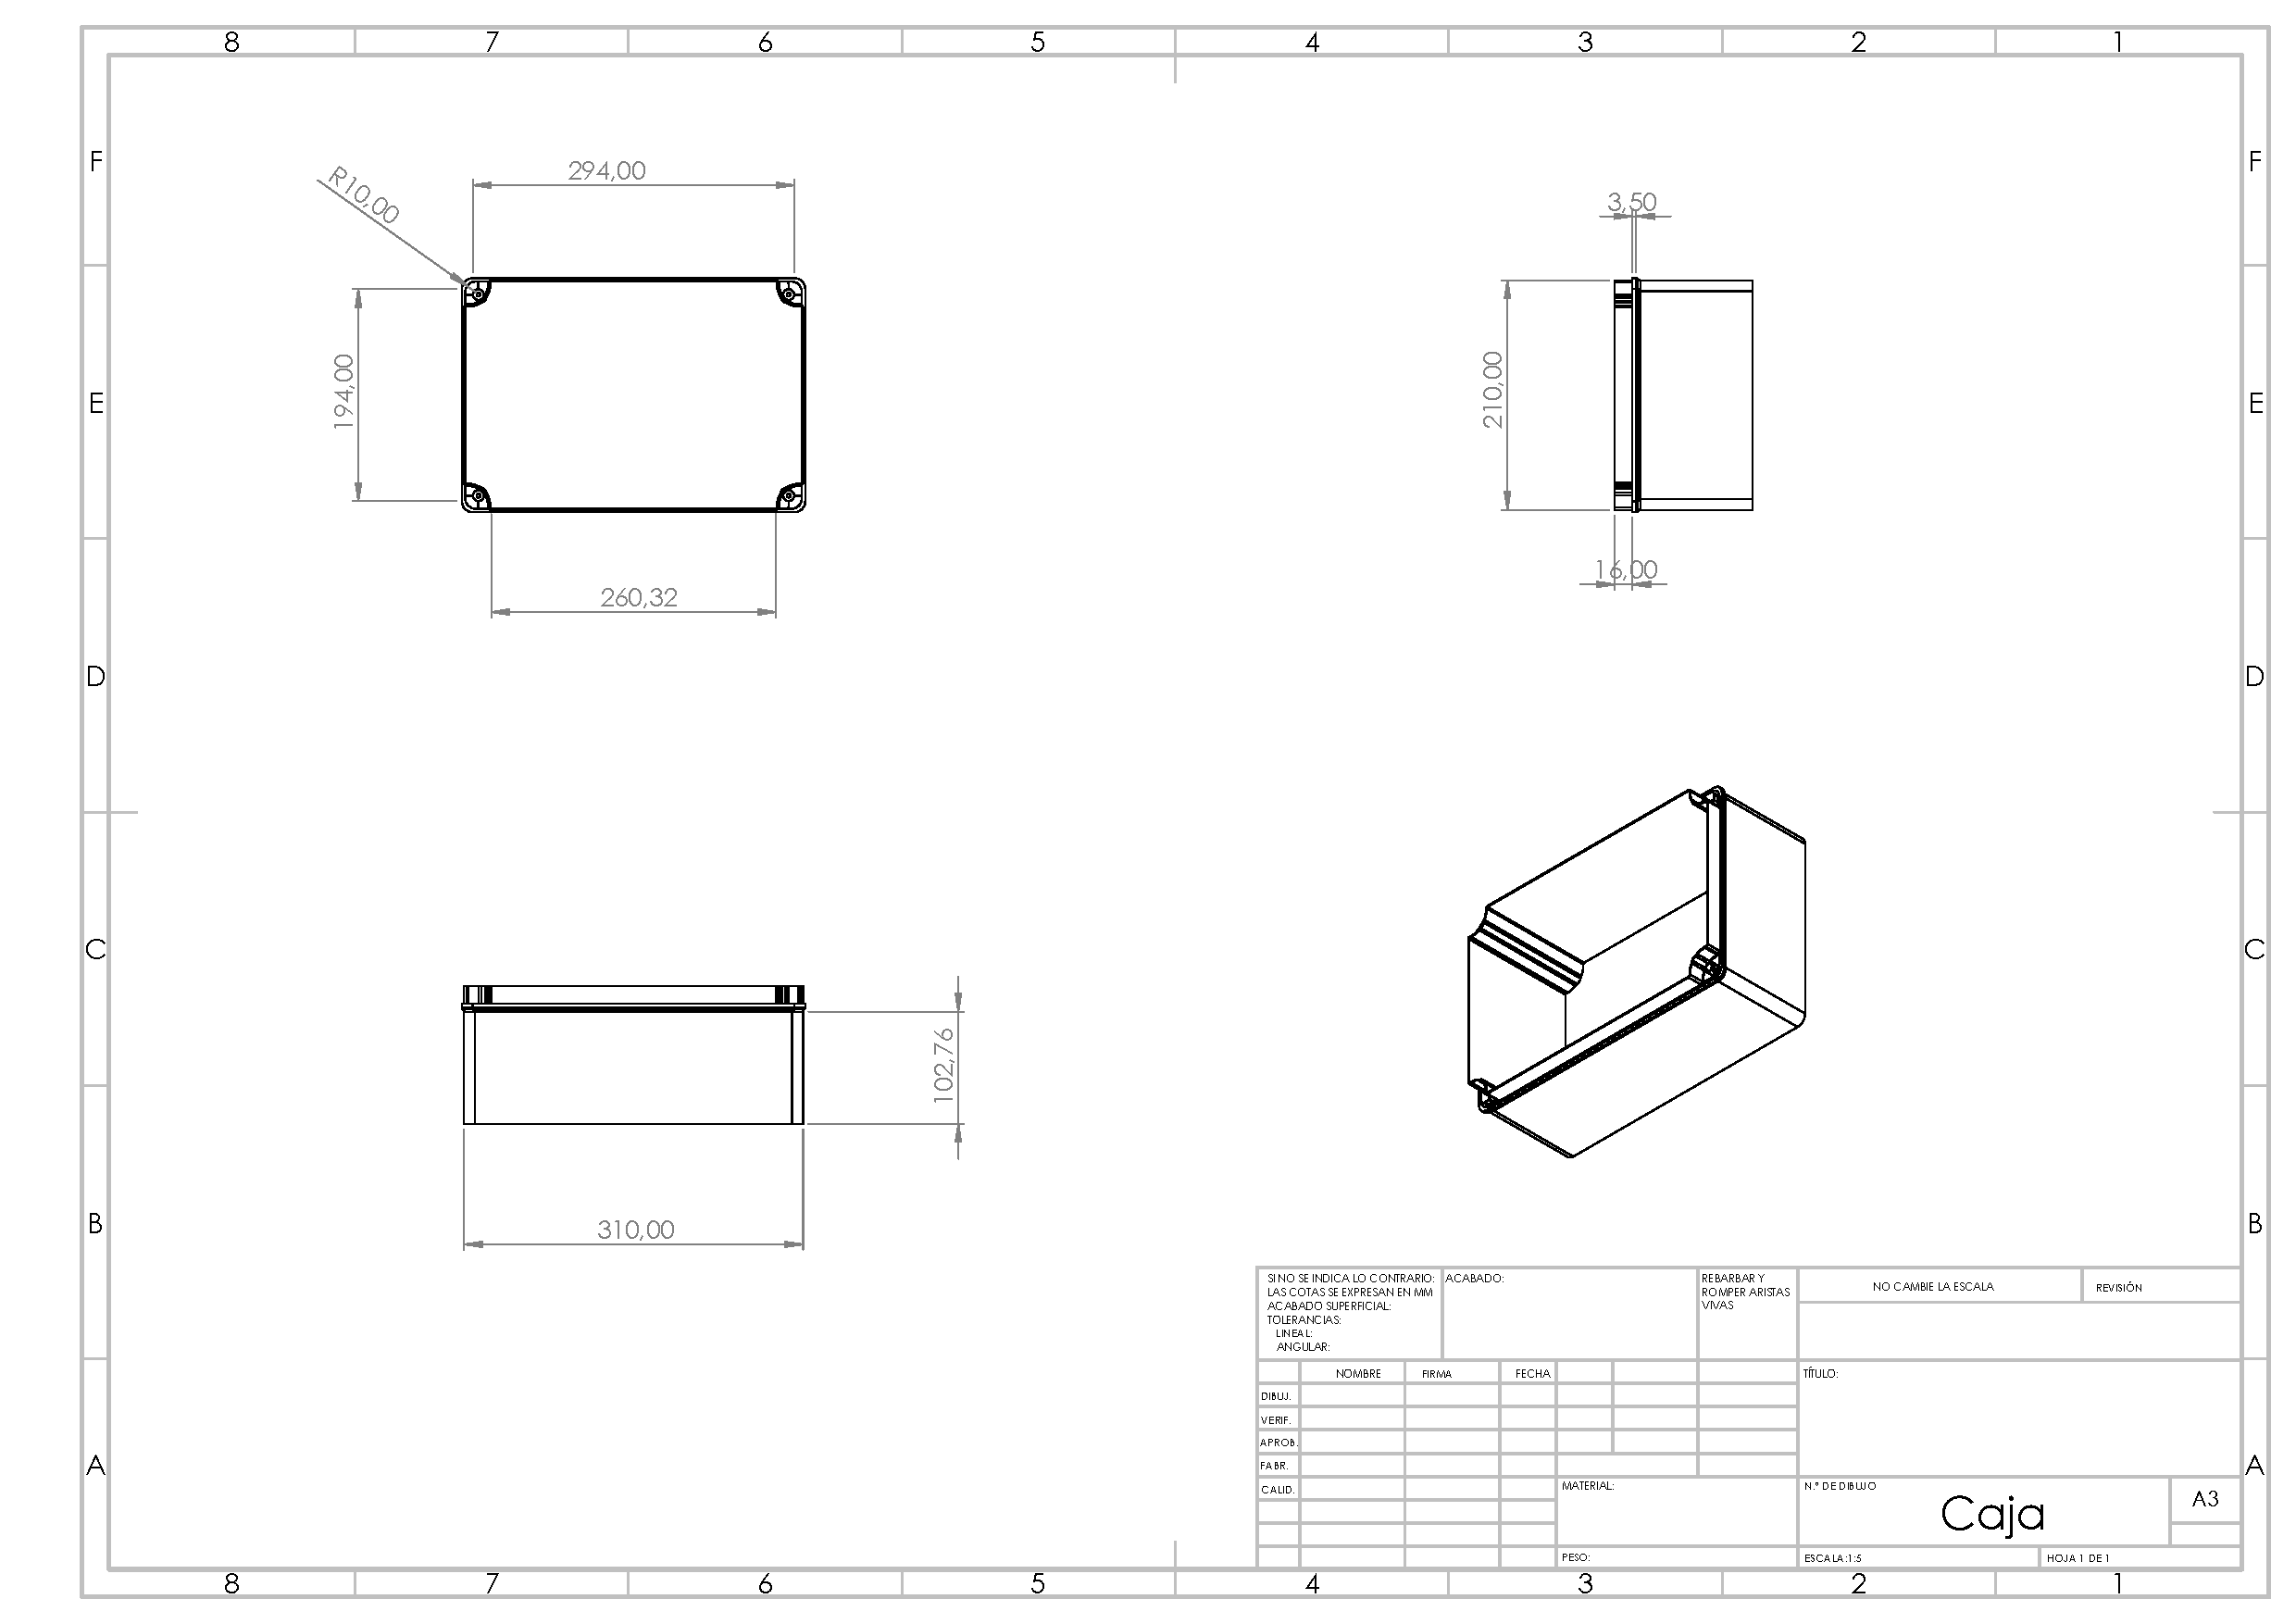
\includegraphics[width=\textwidth]{plano_Caja.pdf}
    \caption{Gabinete de la electrónica (escala 1:5, cotas en mm).}
\end{figure}

\begin{figure}[!htbp]
    \centering
    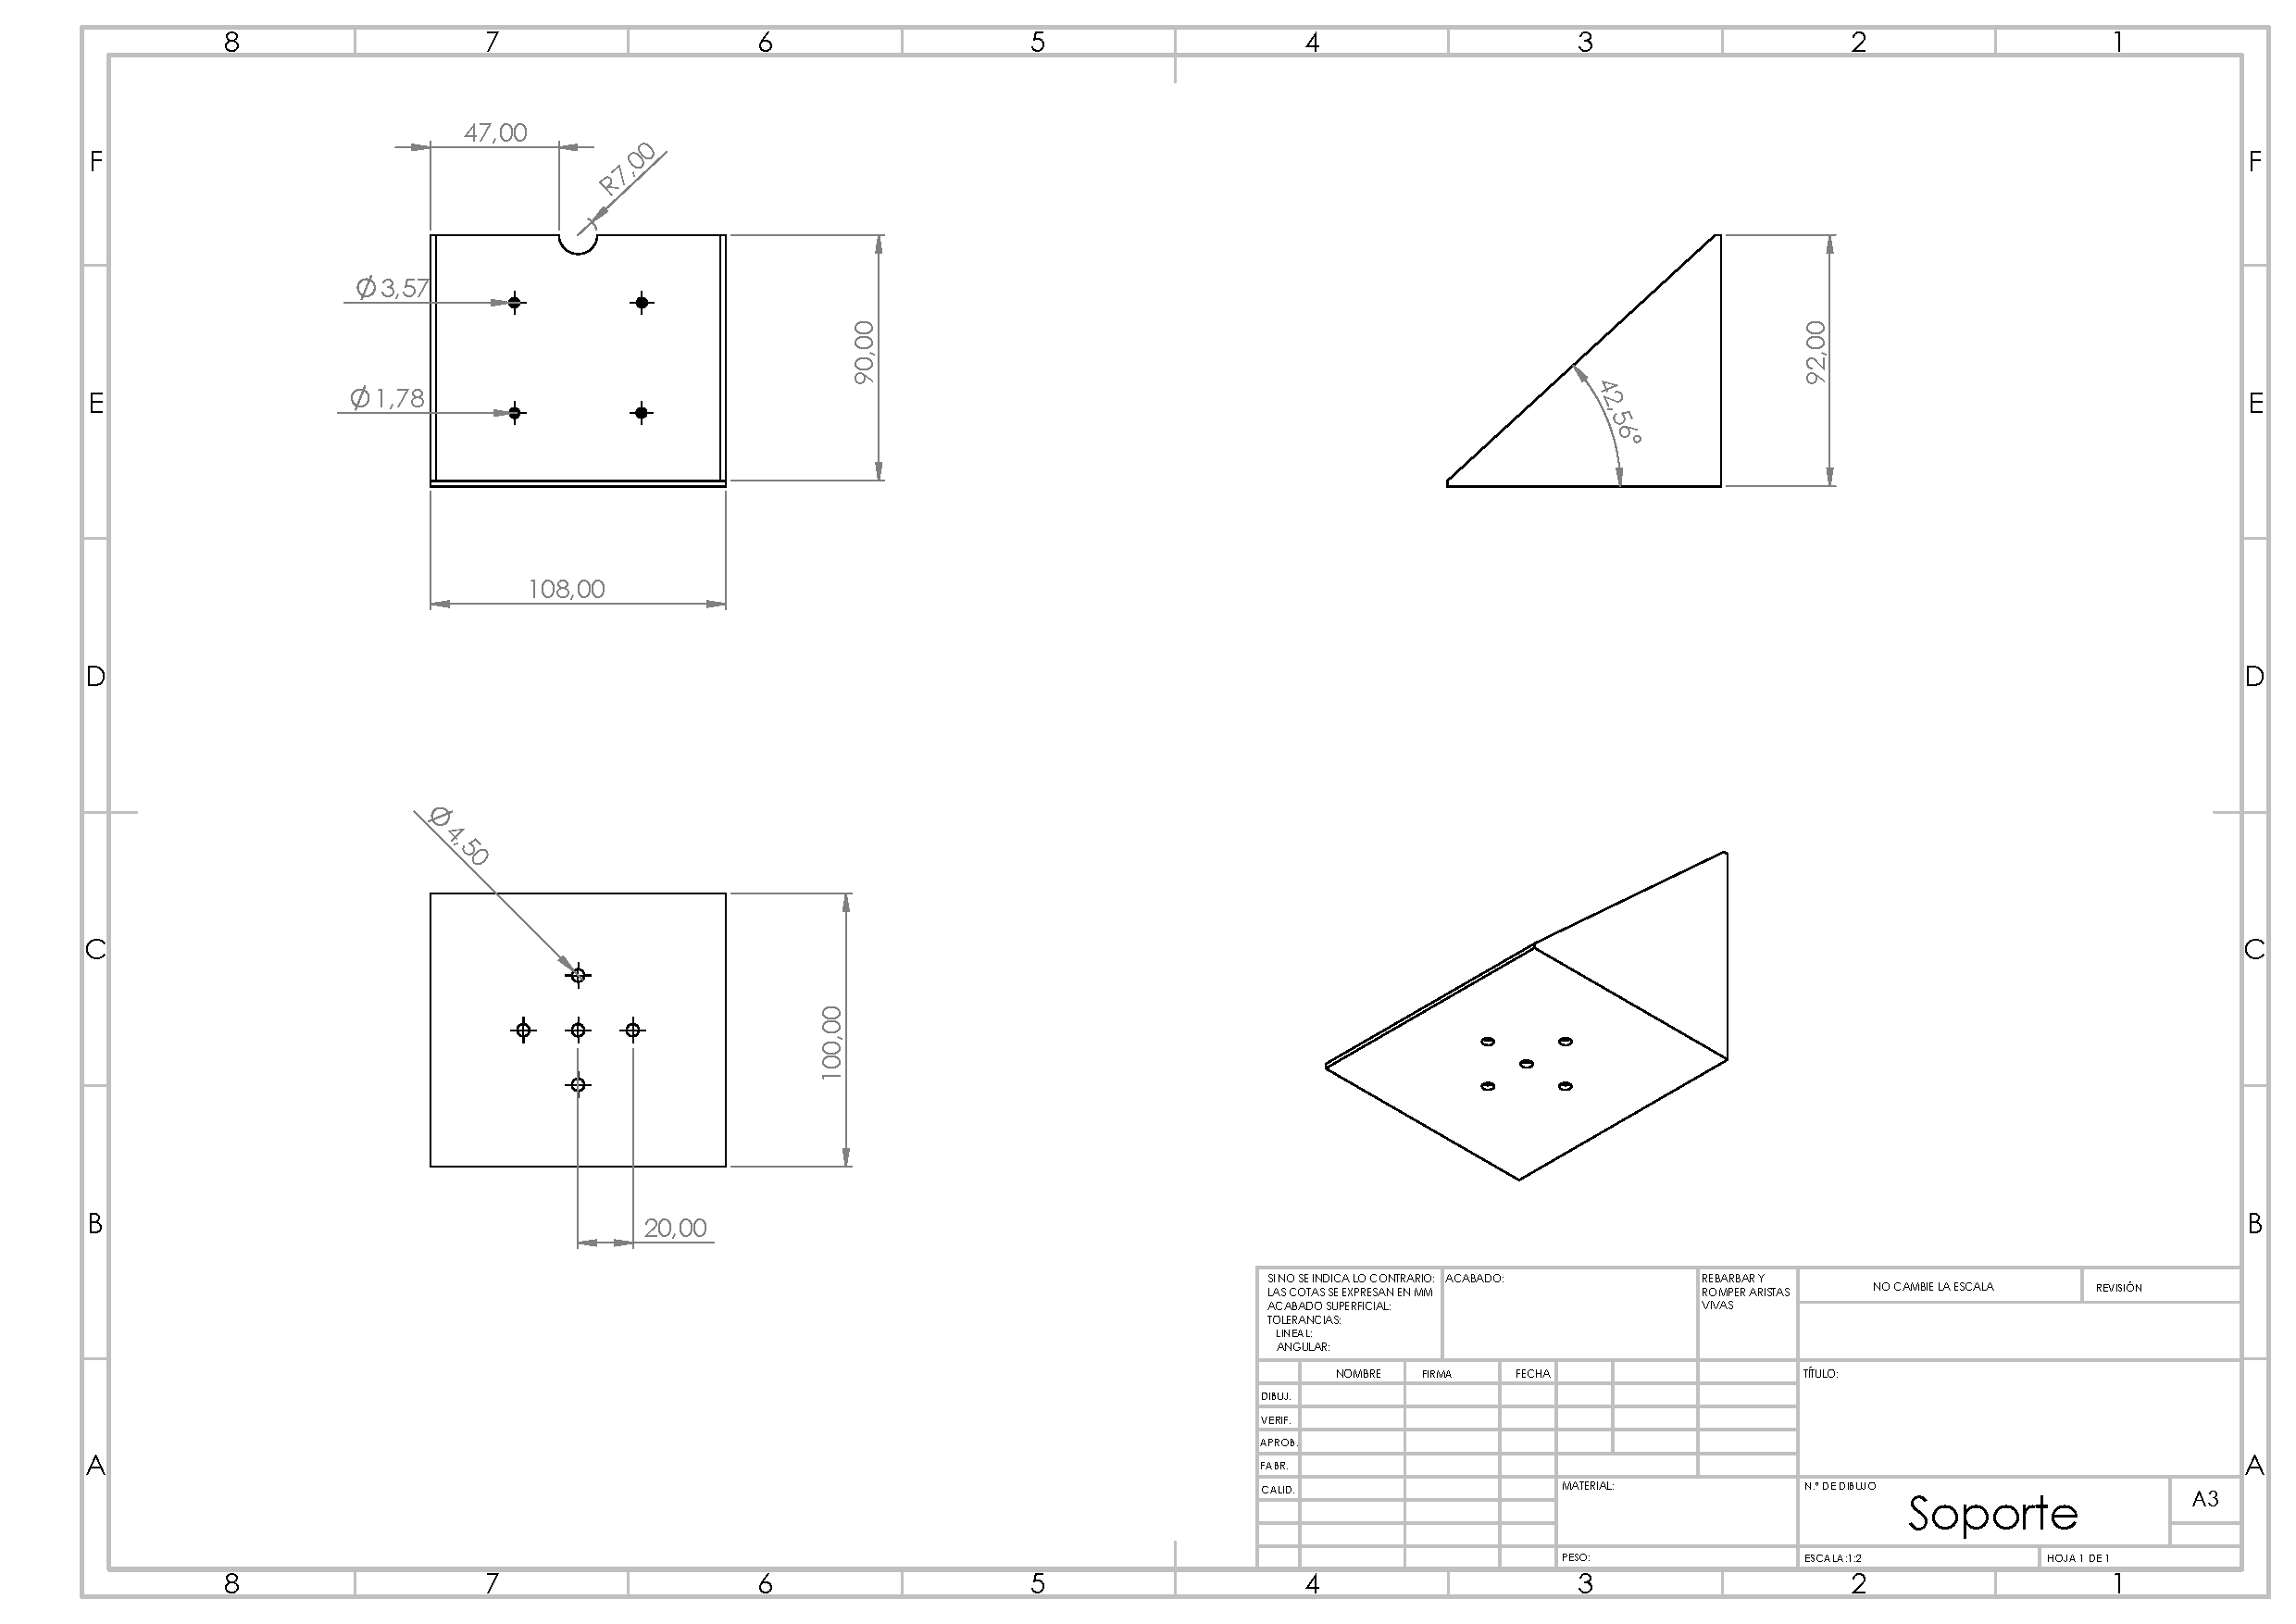
\includegraphics[width=\textwidth]{plano_Soporte.pdf}
    \caption{Soporte del sensor del primer parcial (escala 1:2, cotas en mm).}
\end{figure}

\begin{figure}[!htbp]
    \centering
    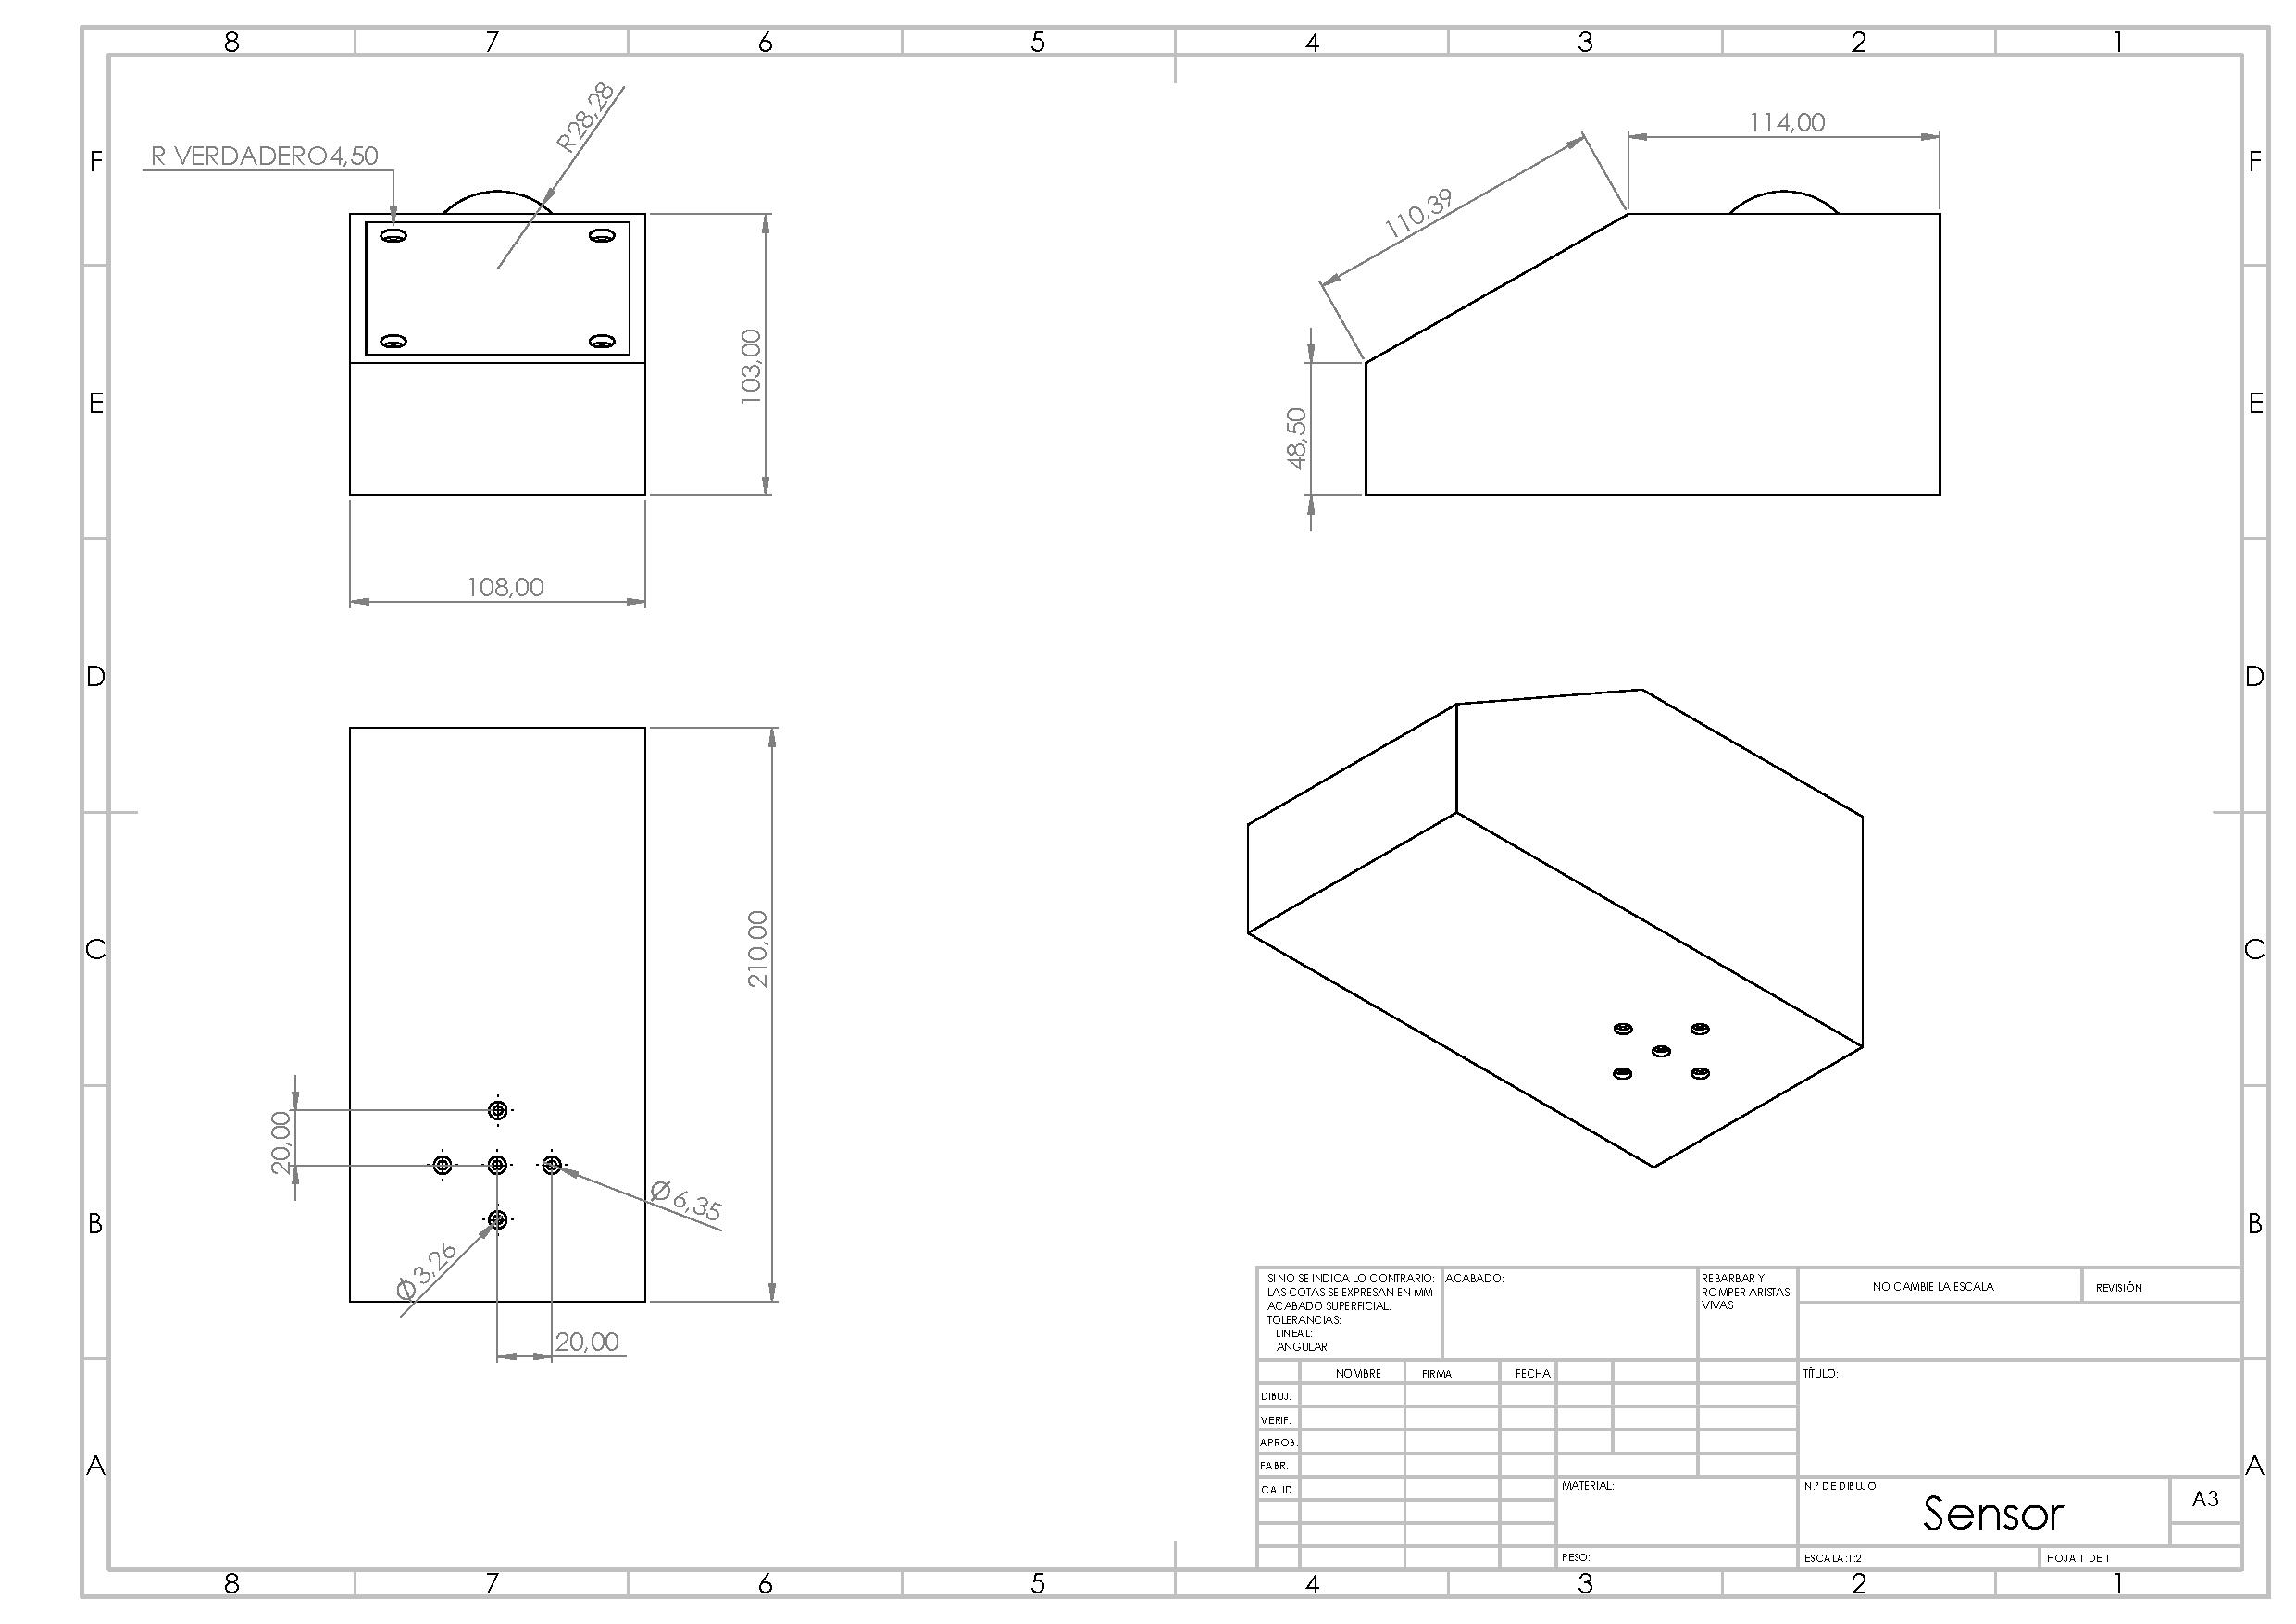
\includegraphics[width=\textwidth]{plano_Sensor.pdf}
    \caption{Pieza «Sensor» del primer parcial (escala 1:2, cotas en mm).}
\end{figure}

\end{document}
